\clearpage
\section{Signal signature and base selection}
\label{sec:signal-signature}

To develop an effective analysis strategy, one must study and exploit the signal kinematics. The production of electroweakinos has unique characteristics that can be leveraged to differentiate the signal from the \gls{sm} background. It is crucial to examine these signal distributions to define a preselection or base cut that retains the maximum signal while rejecting as much background as possible. All the following distributions were generated by weighting the simulation to the Run II luminosity of $\lumi = 135 \fbinv$ and requiring at least one jet in the event with $\pt \geq 30\GeV$ and $\abs{\eta}<2.4$. Any additional selection criteria will be listed in each section, if applicable.

\subsection{Missing Transverse Energy}
\label{subsec:signal-met-mht}

A common property shared by essentially all searches for \gls{dam} is the presence of a \gls{dam} candidate in the production. The identity and properties of the particle (or particles in the case of multiple \gls{dam} candidates) vary, but they do have much in common. In this \gls{susy} search, the \gls{neutralino} is the \gls{dam} candidate, which is a type of \gls{wimp}. A \gls{wimp} is a new elementary particle that interacts via gravity and potentially other forces, not part of the \gls{sm} itself, and is as weak as or weaker than the weak nuclear force, but also non-vanishing in strength. This essentially means that such a candidate is neutral and does not interact via the electromagnetic force. A neutral particle that does not interact electromagnetically or via the strong force (\ie, is colorless) will not be detected and will leave traces in the form of a transverse momentum imbalance, which is referred to as \gls{met} (Missing Transverse Energy or Missing Transverse Momentum). The signal contains two \gls{dam} candidates in the production, which are the \glspl{lsp}, the \glspl{neutralino} \neuto. Therefore, a considerable magnitude of \gls{met} is expected in the signal. As described in Section~\ref{subsec:met}, \gls{mht} is of greater interest, which is highly correlated with \gls{met}, due to the definition of lepton isolation and its use in the background estimation methods. Nonetheless, both $\MET$ and $\mht$ observables will be examined in Figure~\ref{fig:signal-met-mht}.


\begin{figure}[!htb]
\centering
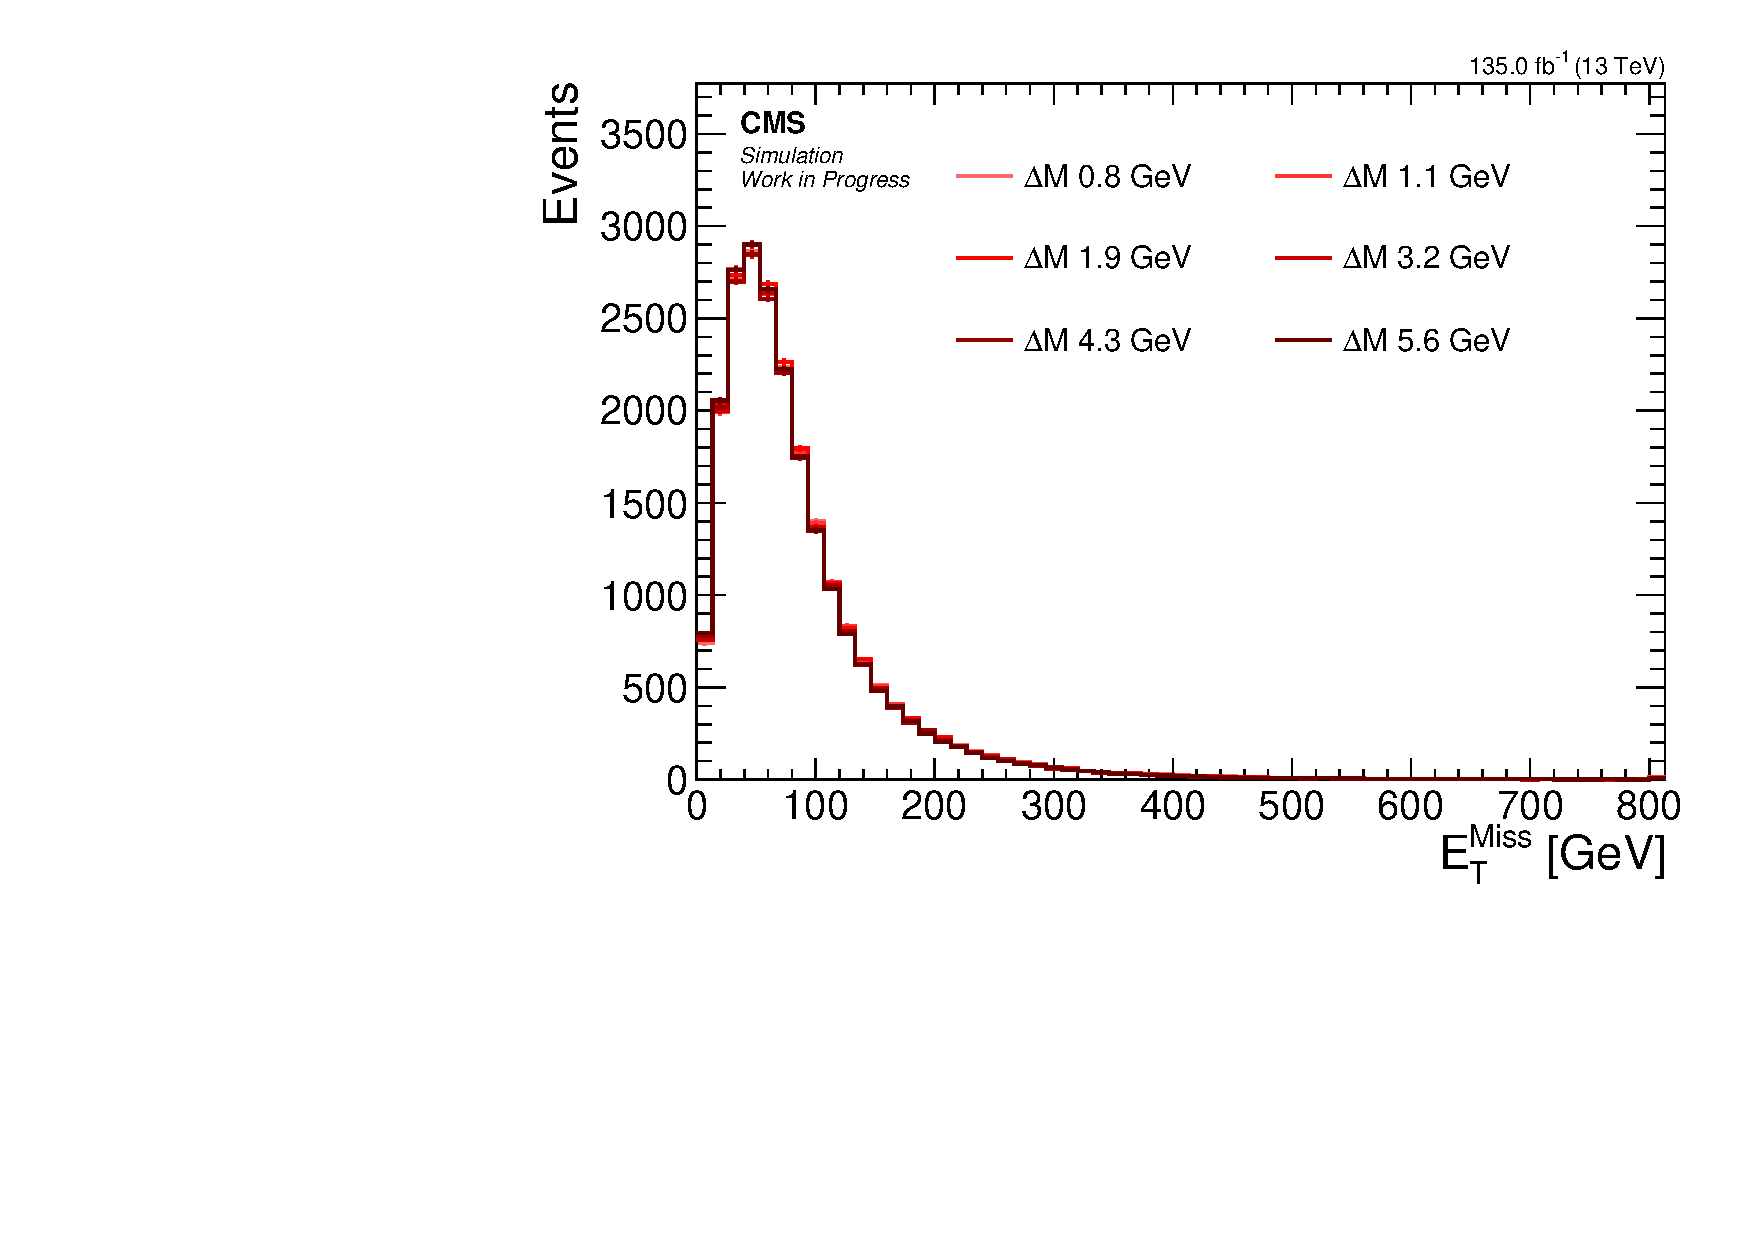
\includegraphics[width=0.48\linewidth]{plots/signal_common_distributions_fixed_mu/none_MET.pdf} \,
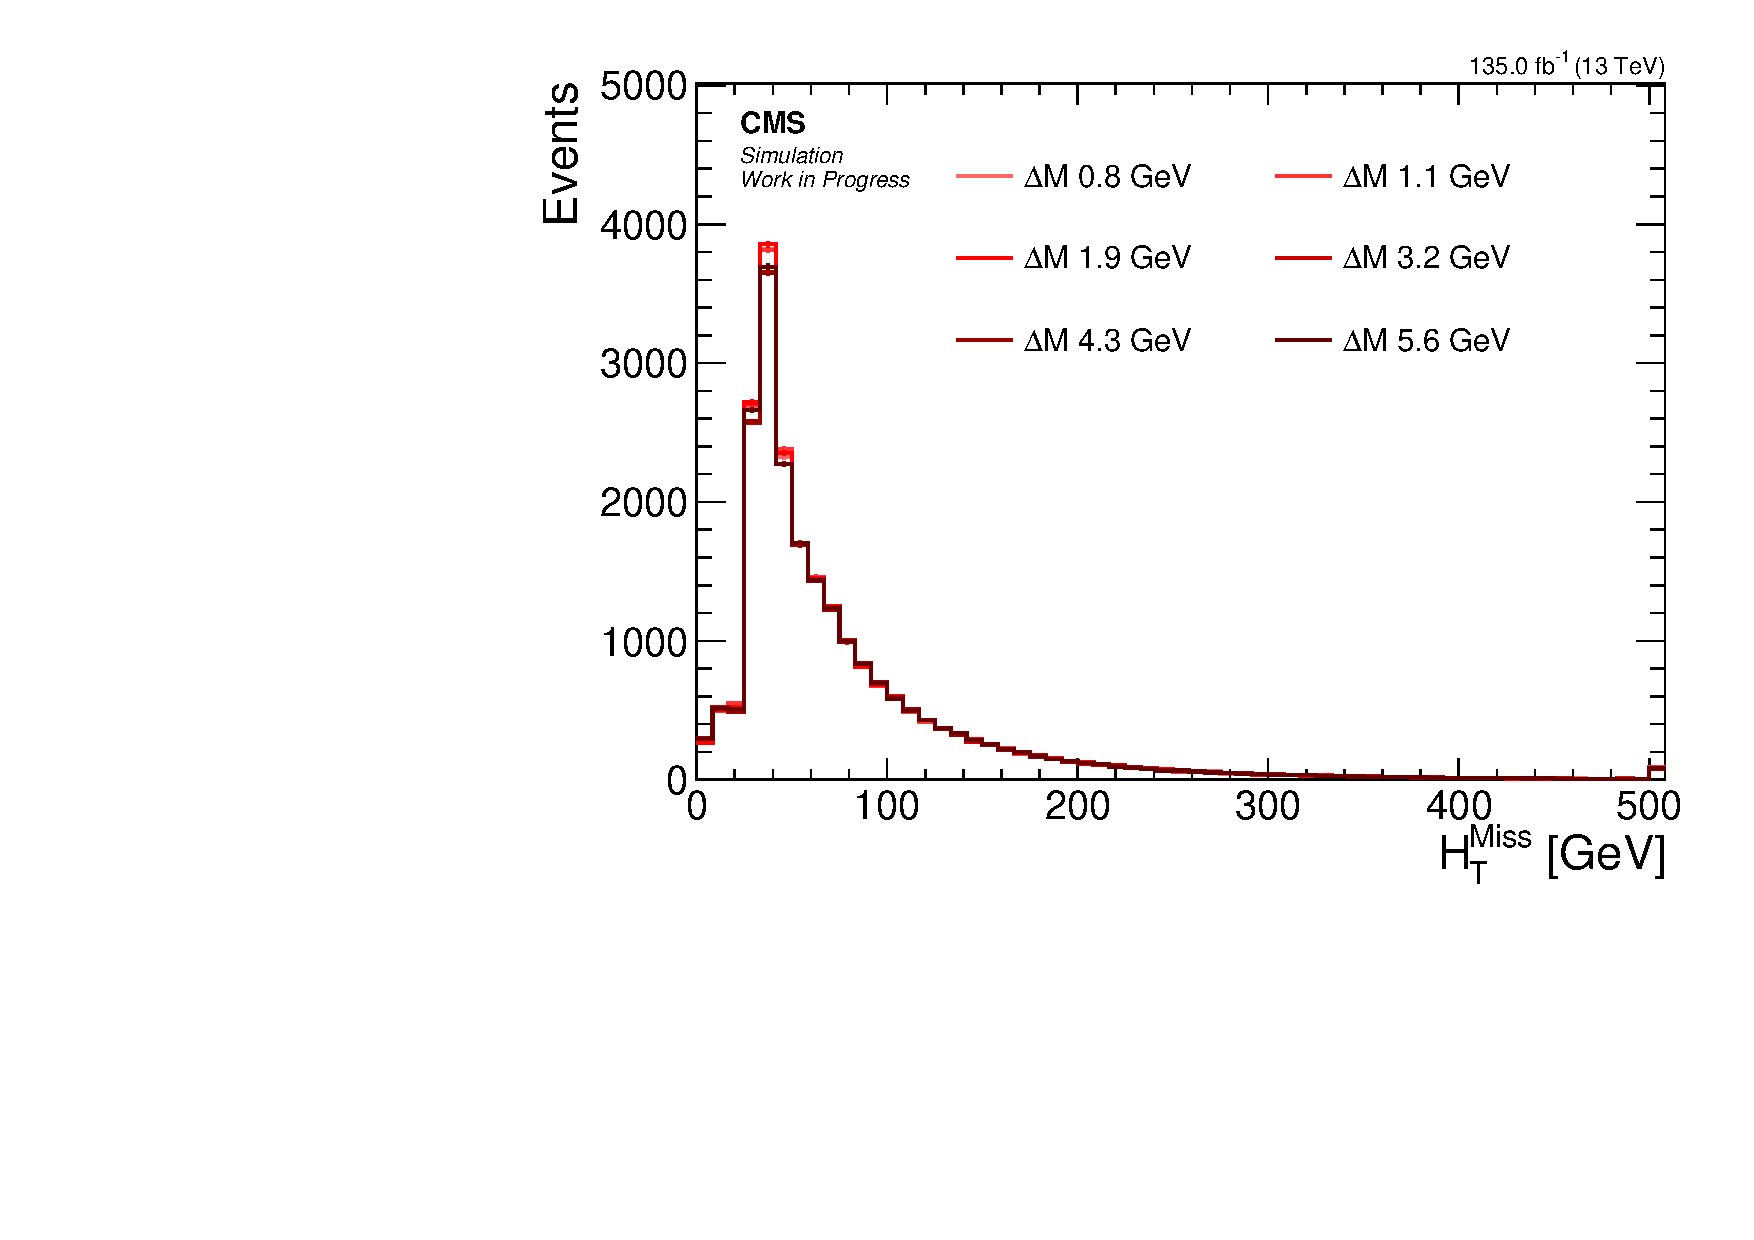
\includegraphics[width=0.48\linewidth]{plots/signal_common_distributions_fixed_mu/none_MHT.pdf}  \\
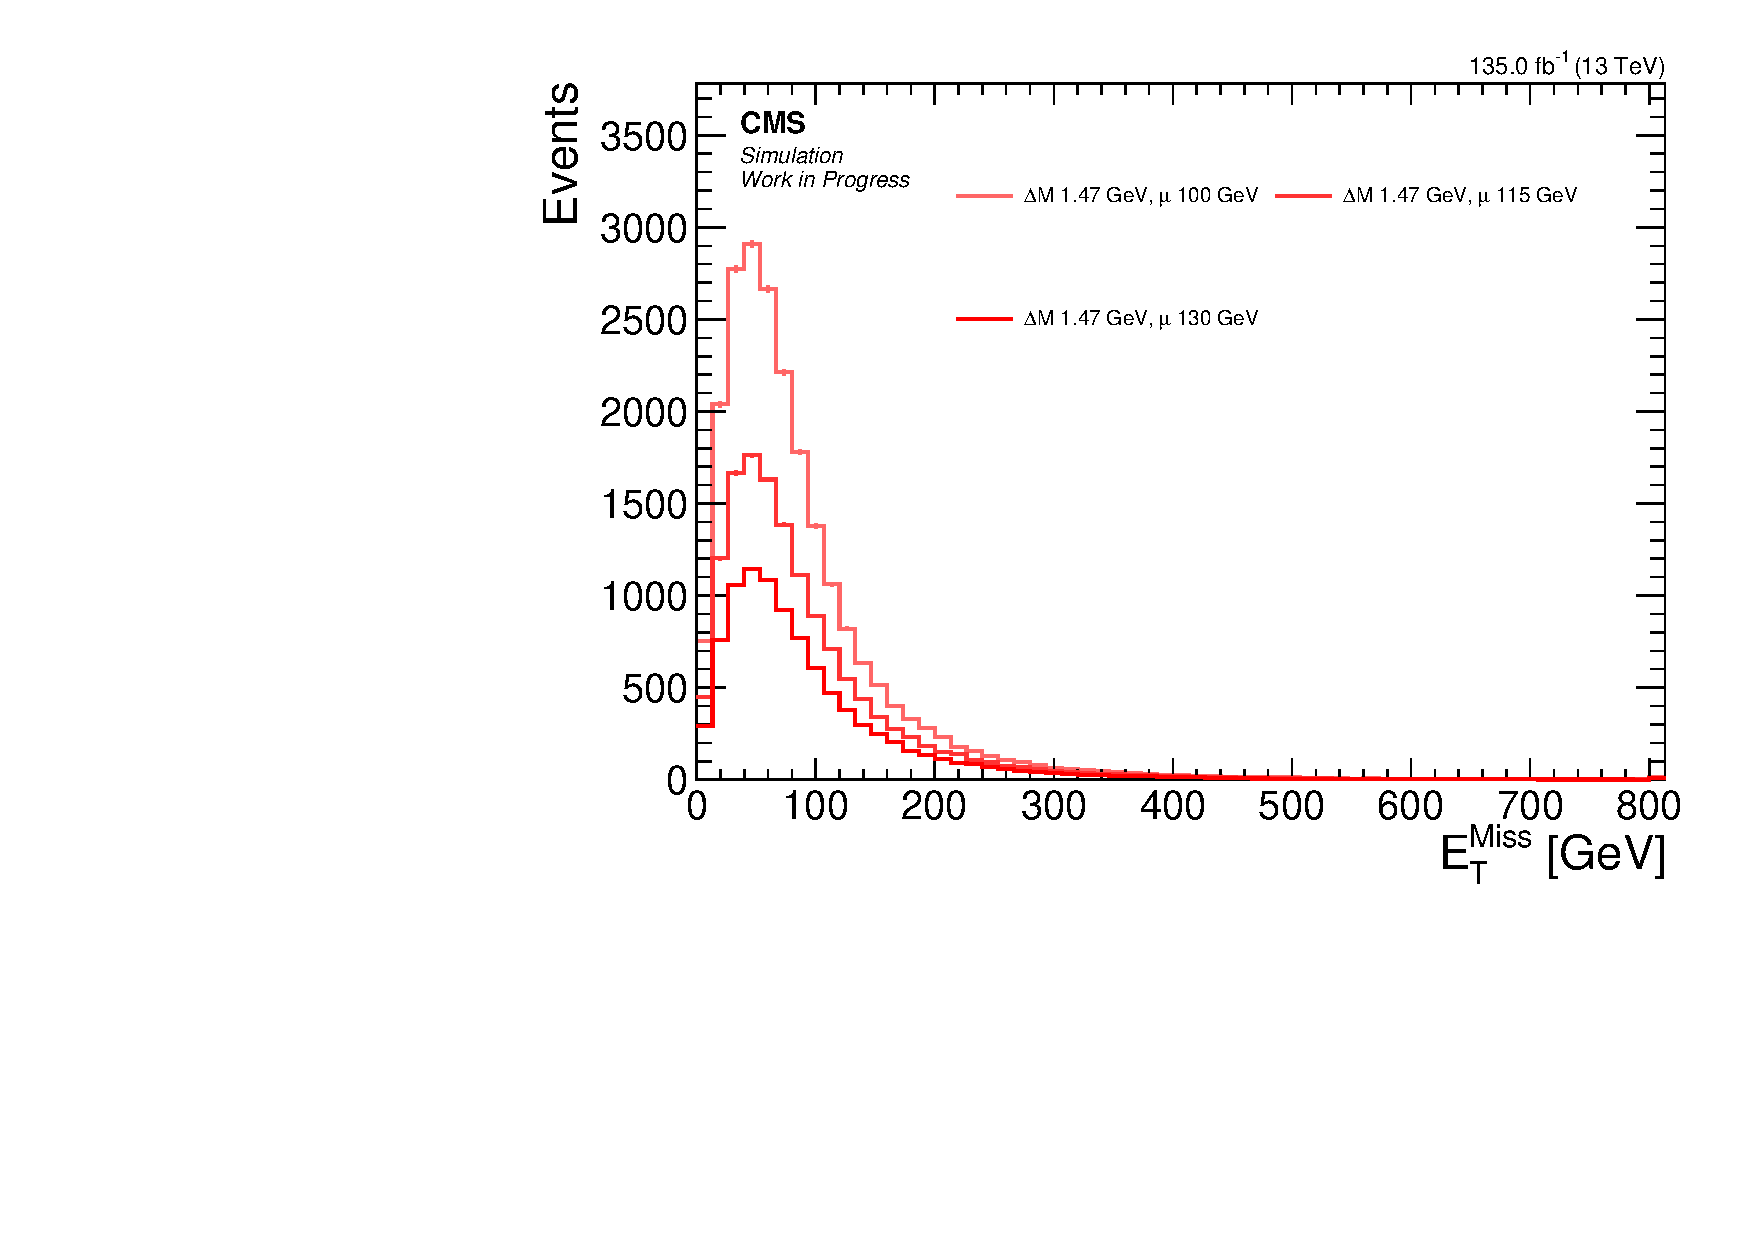
\includegraphics[width=0.48\linewidth]{plots/signal_common_distributions_fixed_dm/none_MET.pdf} \,
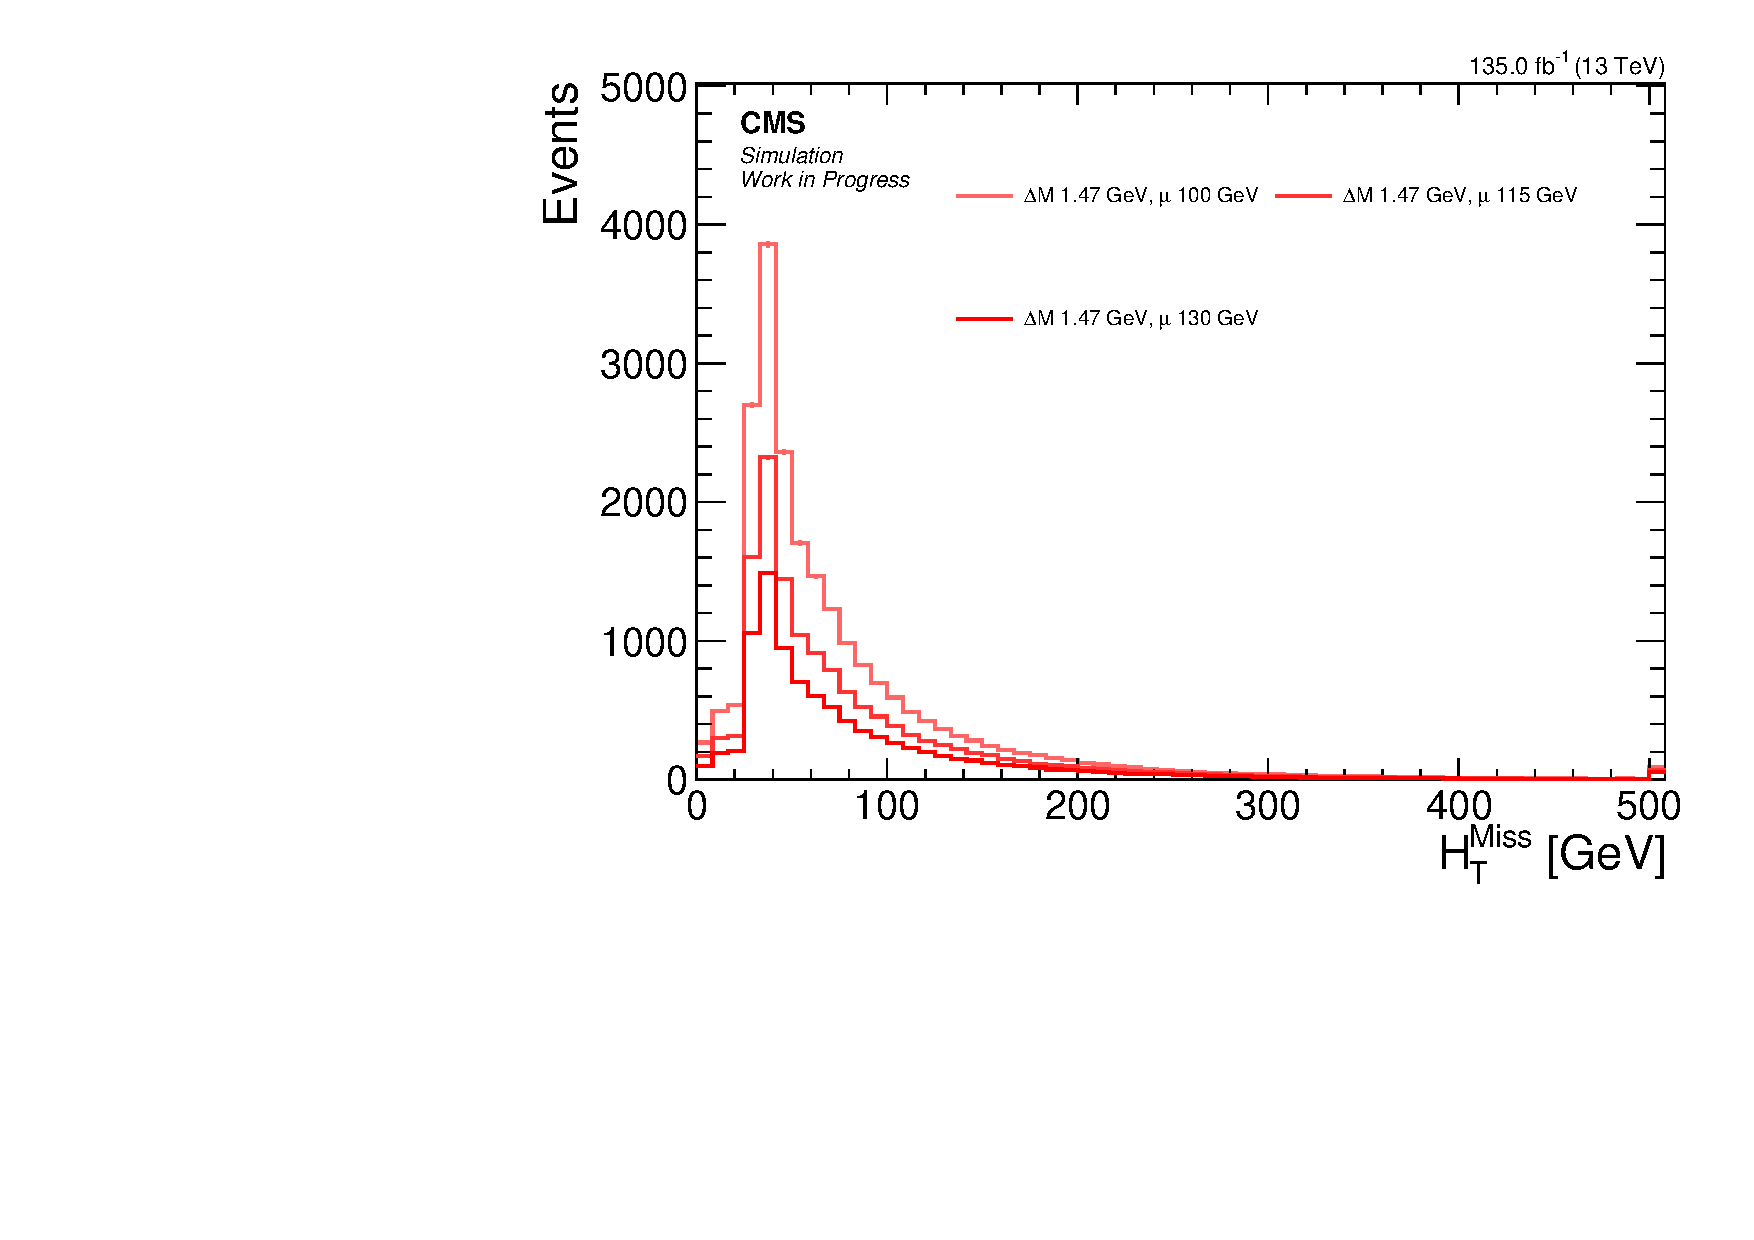
\includegraphics[width=0.48\linewidth]{plots/signal_common_distributions_fixed_dm/none_MHT.pdf}  \\
\caption[Signal $\MET$ and $\mht$ distributions]{ Signal distributions for \MET (left) and \mht (right) comparing various $\dm$ with a fixed higgsino parameter $\mu=100\GeV$ (upper), and comparing various higgsino parameters $\mu$ with fixed $\dm=1.47\GeV$ (lower).}
\label{fig:signal-met-mht}
\end{figure}

As expected, $\MET$ and $\mht$ are hardly affected by the different choices for \dm, while the higgsino parameter $\mu$ affects the distributions mainly through its lower production cross section for higher higgsino parameter $\mu$. The region of interest for triggering purposes is located at $\mht\geq 220$, as discussed in Section~\ref{sec:trigger}. Although this is a harsh and inefficient cut, it is necessary to consider the \gls{sm} background in both regions of $\mht < 220$ and $\mht\geq 220$ to conclude that most of the sensitivity comes from the $\mht\geq 220$ region, as the production of real \gls{mht} (or \gls{met}) results from the production of neutrinos in the event, which are much less common than \gls{qcd} events that dominate the $\mht < 220$ region. Therefore, a cut at $\mht\geq 220$ might be inefficient, but it results in high sensitivity.

\subsection{Jets and hardronic activity}

To maximize the boost of the \glspl{neutralino} \neuto that contribute to the \gls{mht} and drive sensitivity in the high \gls{mht} region, it is desirable to maximize their transverse momentum \gls{pt}. A widely used method is to include an \gls{isr} jet in the event. An \gls{isr} jet is created when one of the incoming protons emits radiation (such as a photon or a gluon) before the interaction. If a jet with sufficiently high \gls{pt} is emitted, the remainder of the interaction is recoiled against this jet and imparts momentum to it in the opposite direction. As a result, the boosted \glspl{neutralino} \neuto will have higher \gls{mht}. As described in Section~\ref{subsec:jets}, the jets are required to have $\pt \geq 30\GeV$ and be located within the tracker acceptance $\left(\abs{\eta}<2.4\right)$. At least one such jet is required in each event. The distributions of the number of jets and the leading jet \pt are displayed in Figure~\ref{fig:signal-njets-ljpt}.

\begin{figure}[!htb]
\centering
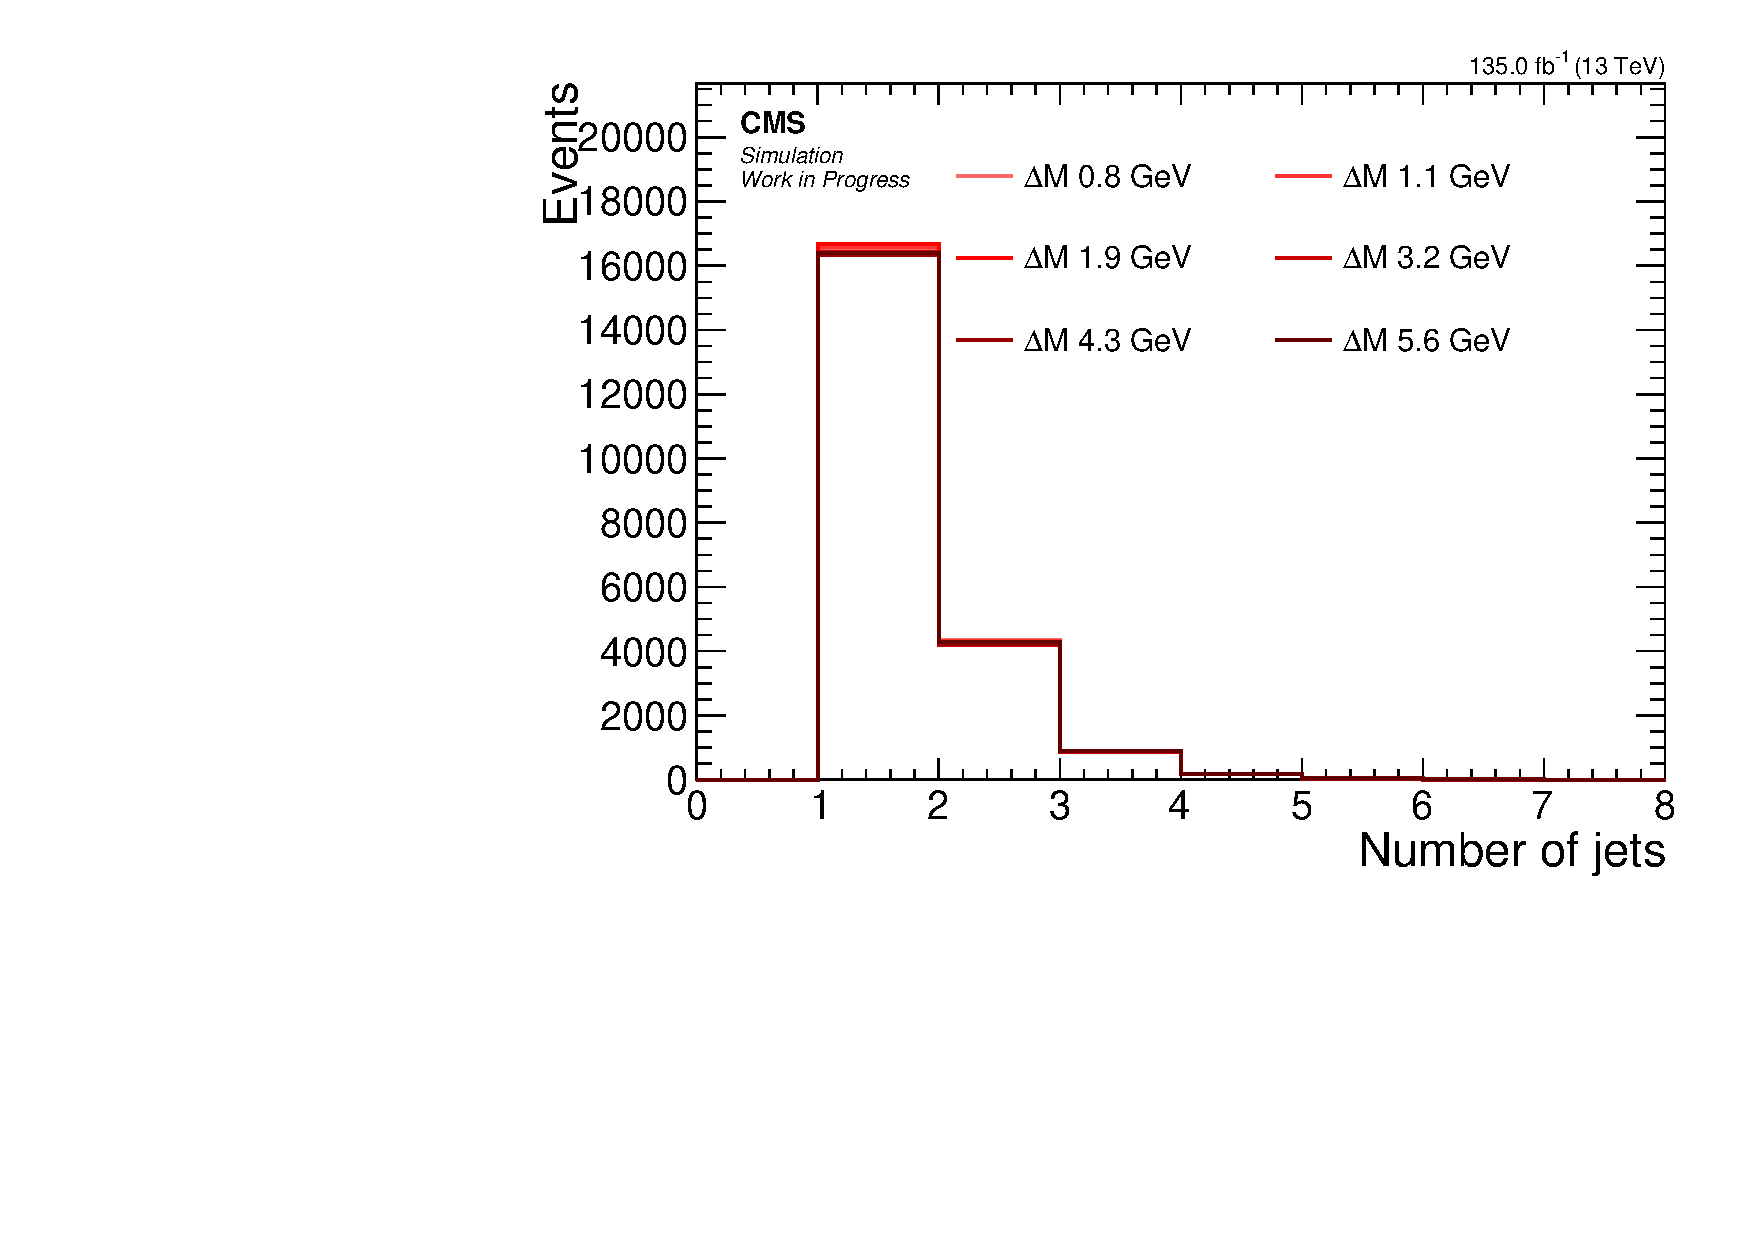
\includegraphics[width=0.48\linewidth]{plots/signal_common_distributions_fixed_mu/none_NJets.pdf} \,
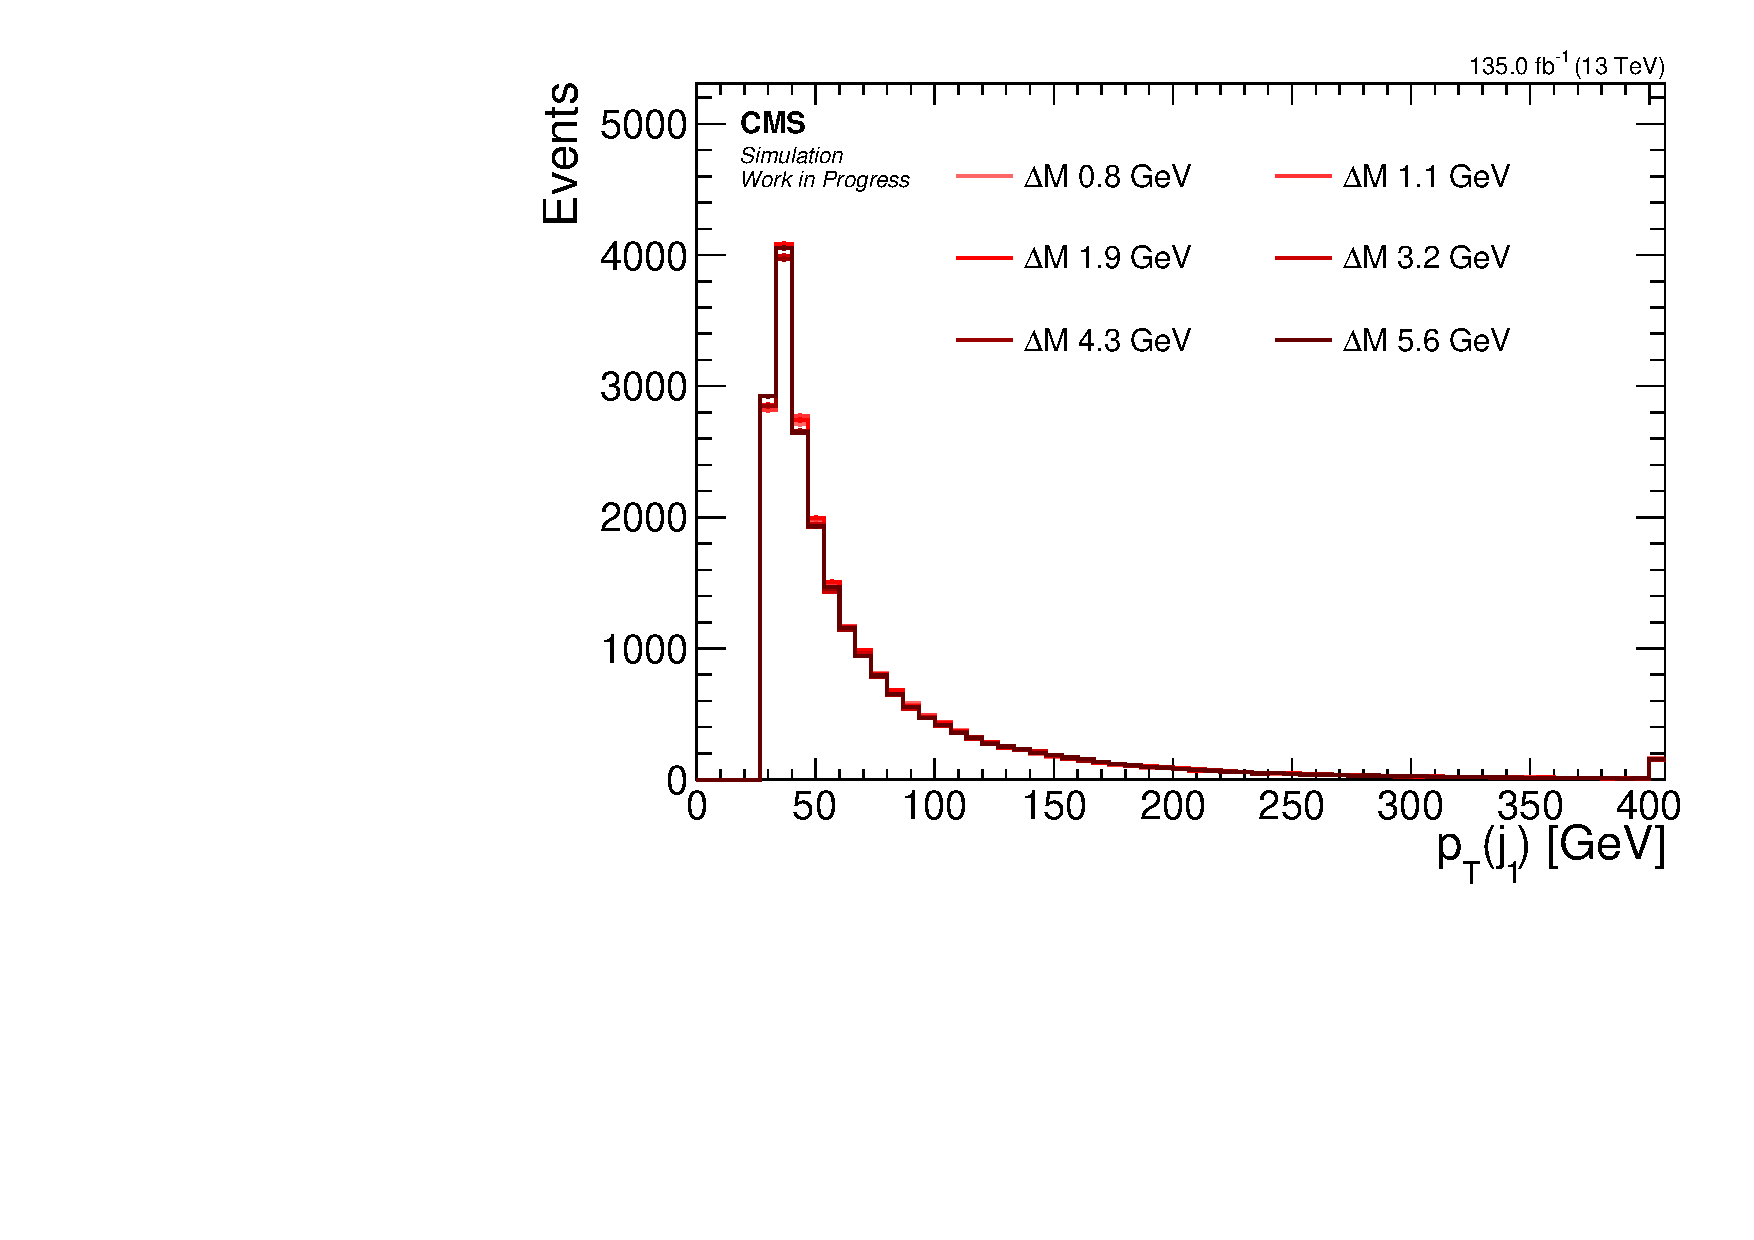
\includegraphics[width=0.48\linewidth]{plots/signal_common_distributions_fixed_mu/none_LeadingJetPt.pdf}  \\
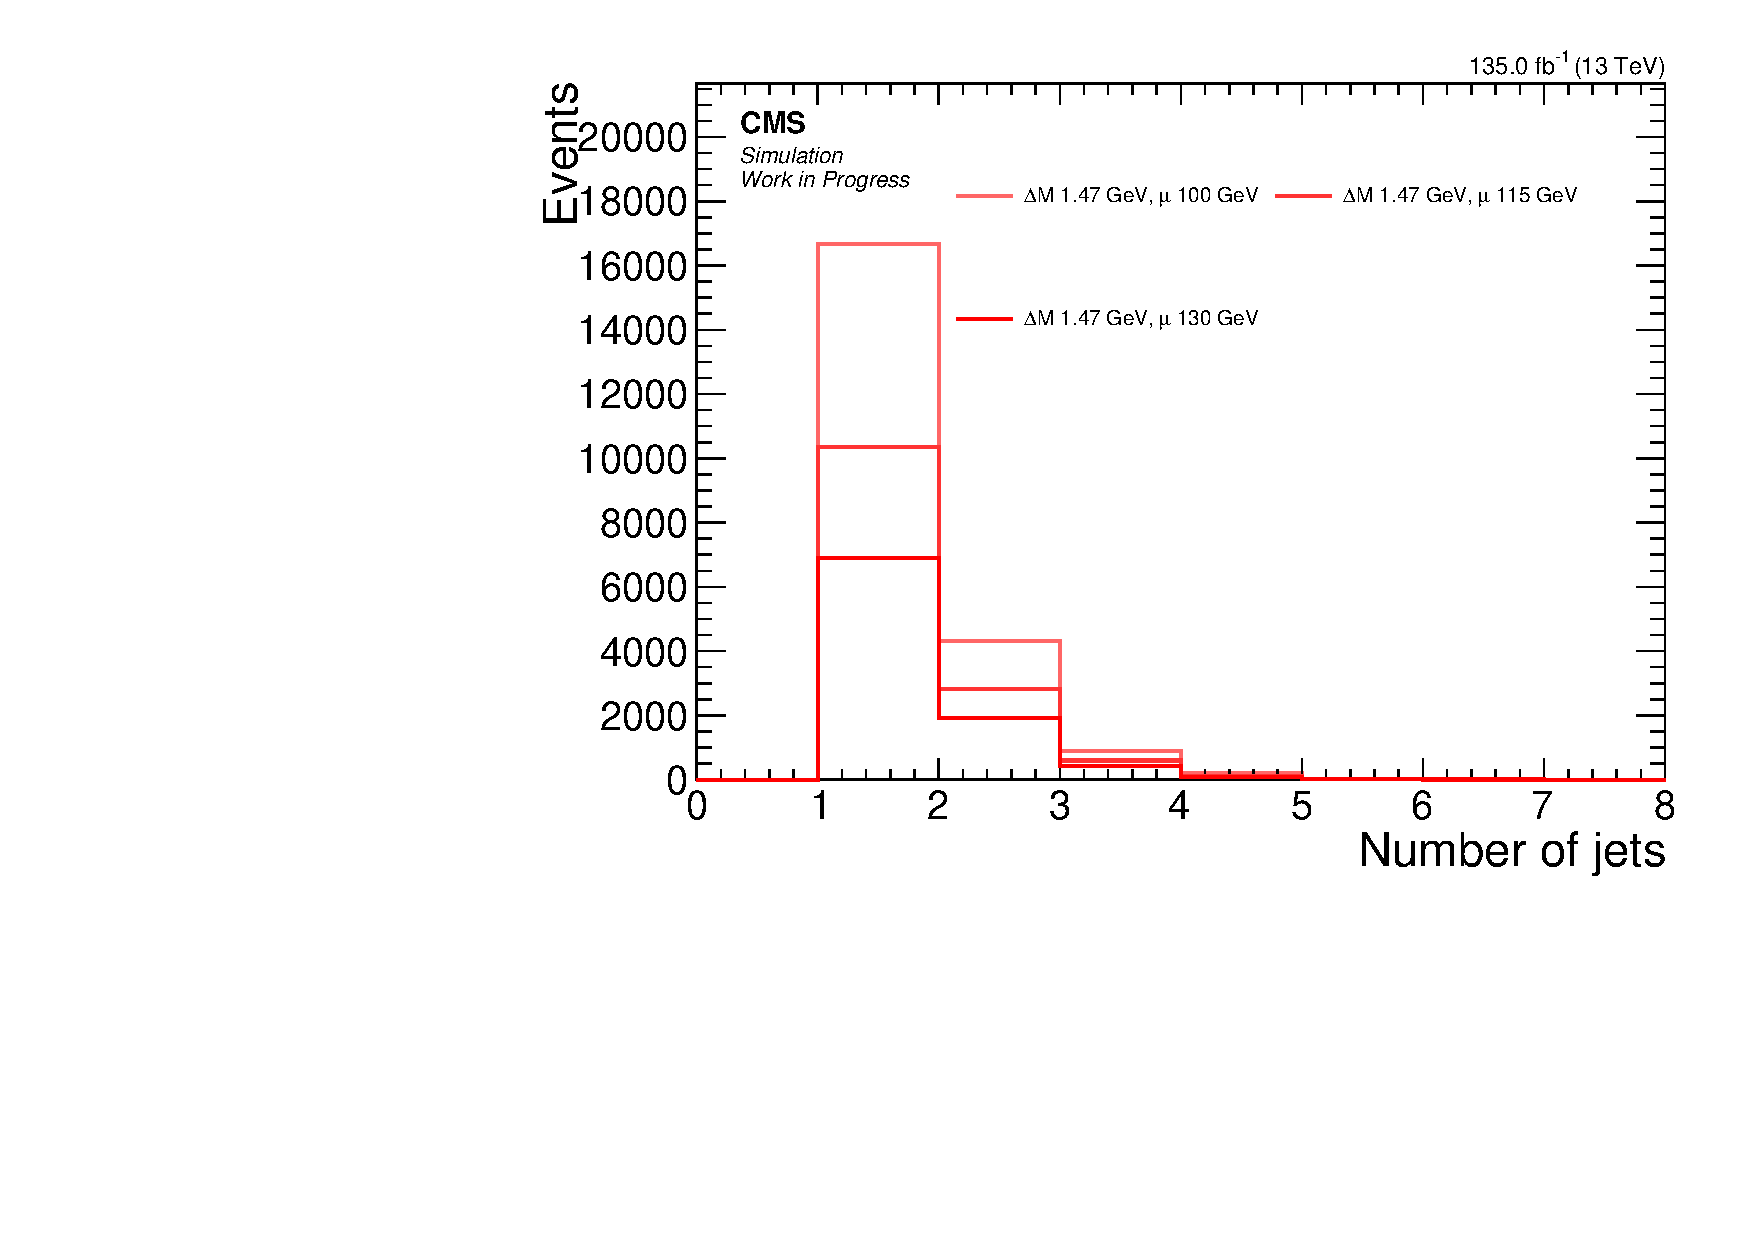
\includegraphics[width=0.48\linewidth]{plots/signal_common_distributions_fixed_dm/none_NJets.pdf} \,
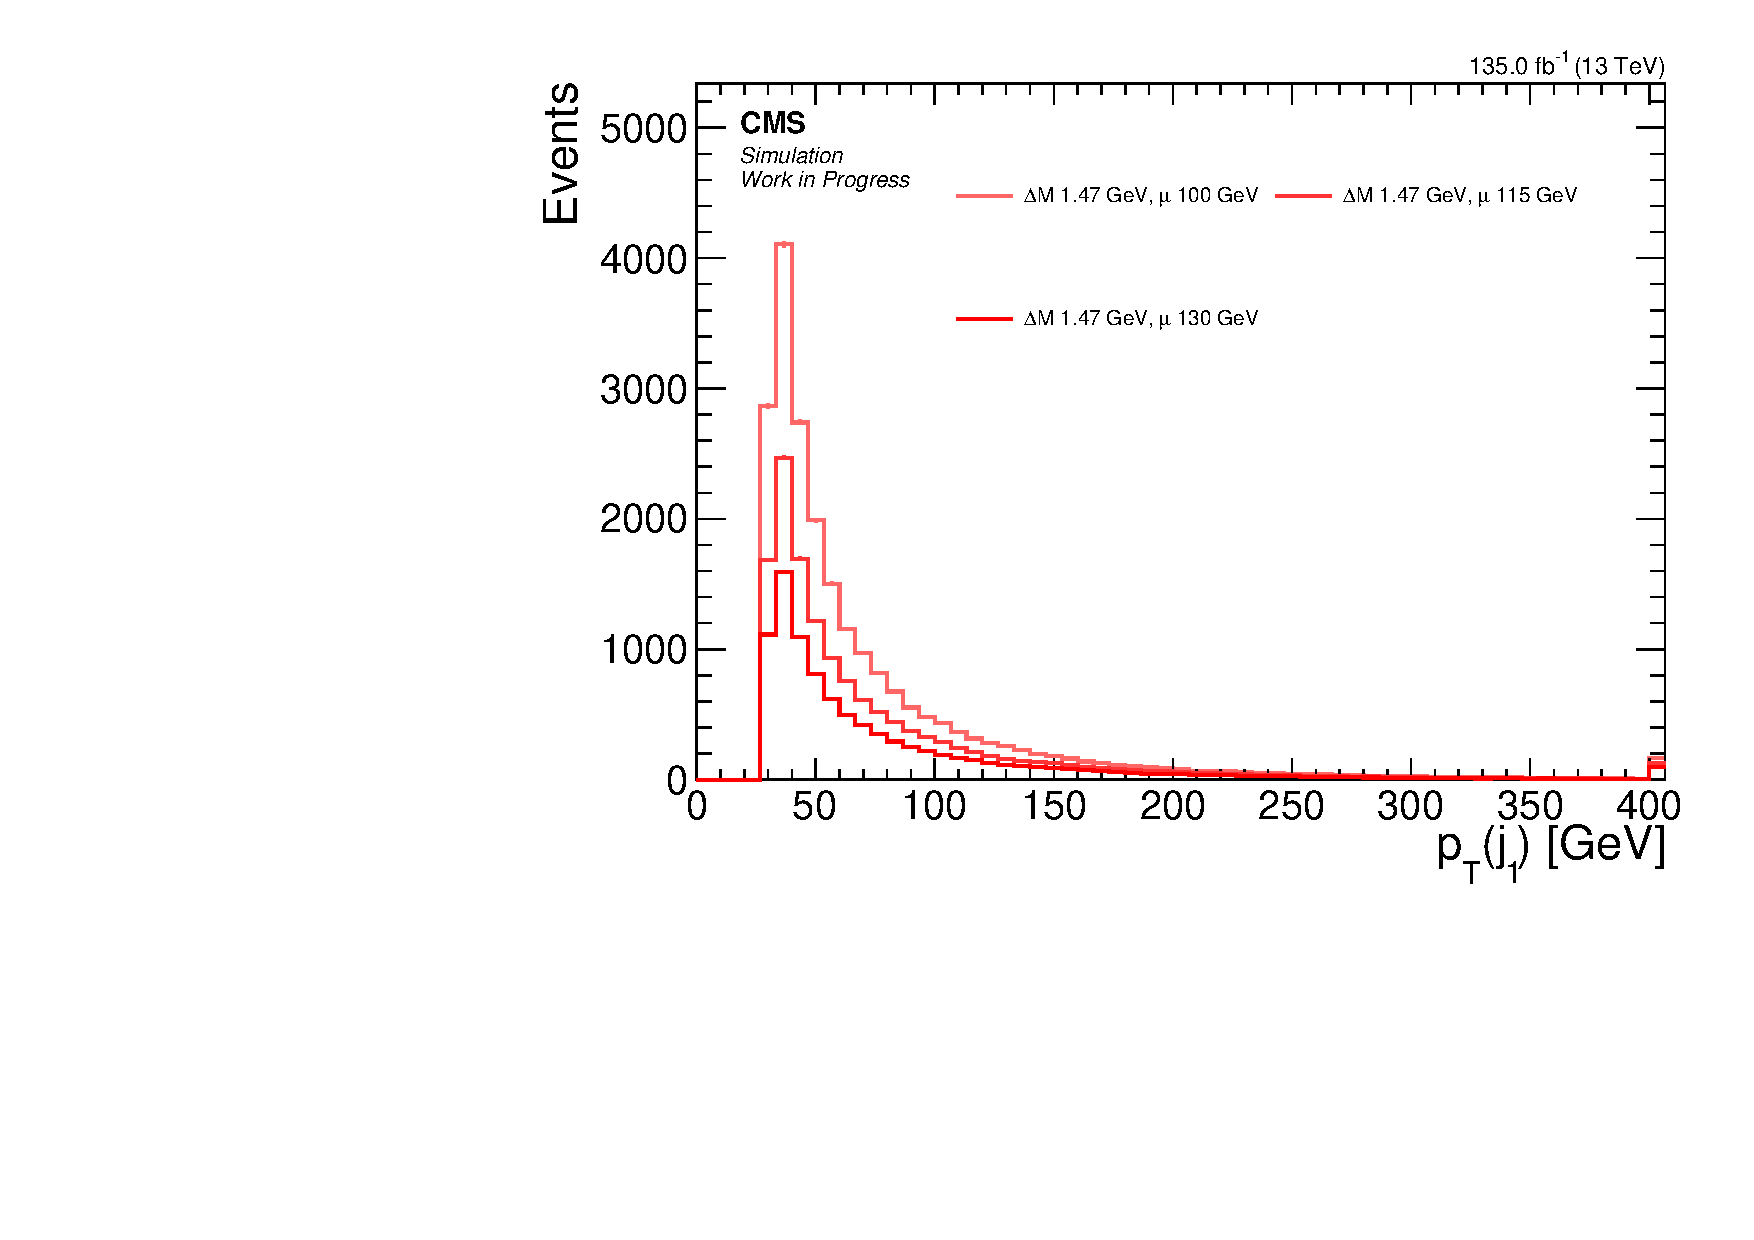
\includegraphics[width=0.48\linewidth]{plots/signal_common_distributions_fixed_dm/none_LeadingJetPt.pdf}  \\
\caption[Signal \emph{number of jets} and \emph{leading jet \pt} distributions]{ Signal distributions for \emph{number of jets} (left) and \emph{leading jet \pt} (right) comparing various $\dm$ with a fixed higgsino parameter $\mu=100\GeV$ (upper), and comparing various higgsino parameters $\mu$ with fixed $\dm=1.47\GeV$ (lower).}
\label{fig:signal-njets-ljpt}
\end{figure}

The signal signature does not include a \PQb-jet, that is, a jet resulting from a bottom quark hadronization (either resulting from a top quark or not). This knowledge is exploited by vetoing \PQb-tagged jets in the event. As described in Section~\ref{subsec:jets}, the \DEEPCSV bottom flavor tagging discriminant with a medium working point is used. The majority of the signal can be seen in the 0 bin, and thus any \PQb-tagged jet will be vetoed, retaining most of the signal but rejecting a lot of \gls{sm} background, such as that arising from \ttbar events.

\begin{figure}[!htb]
\centering
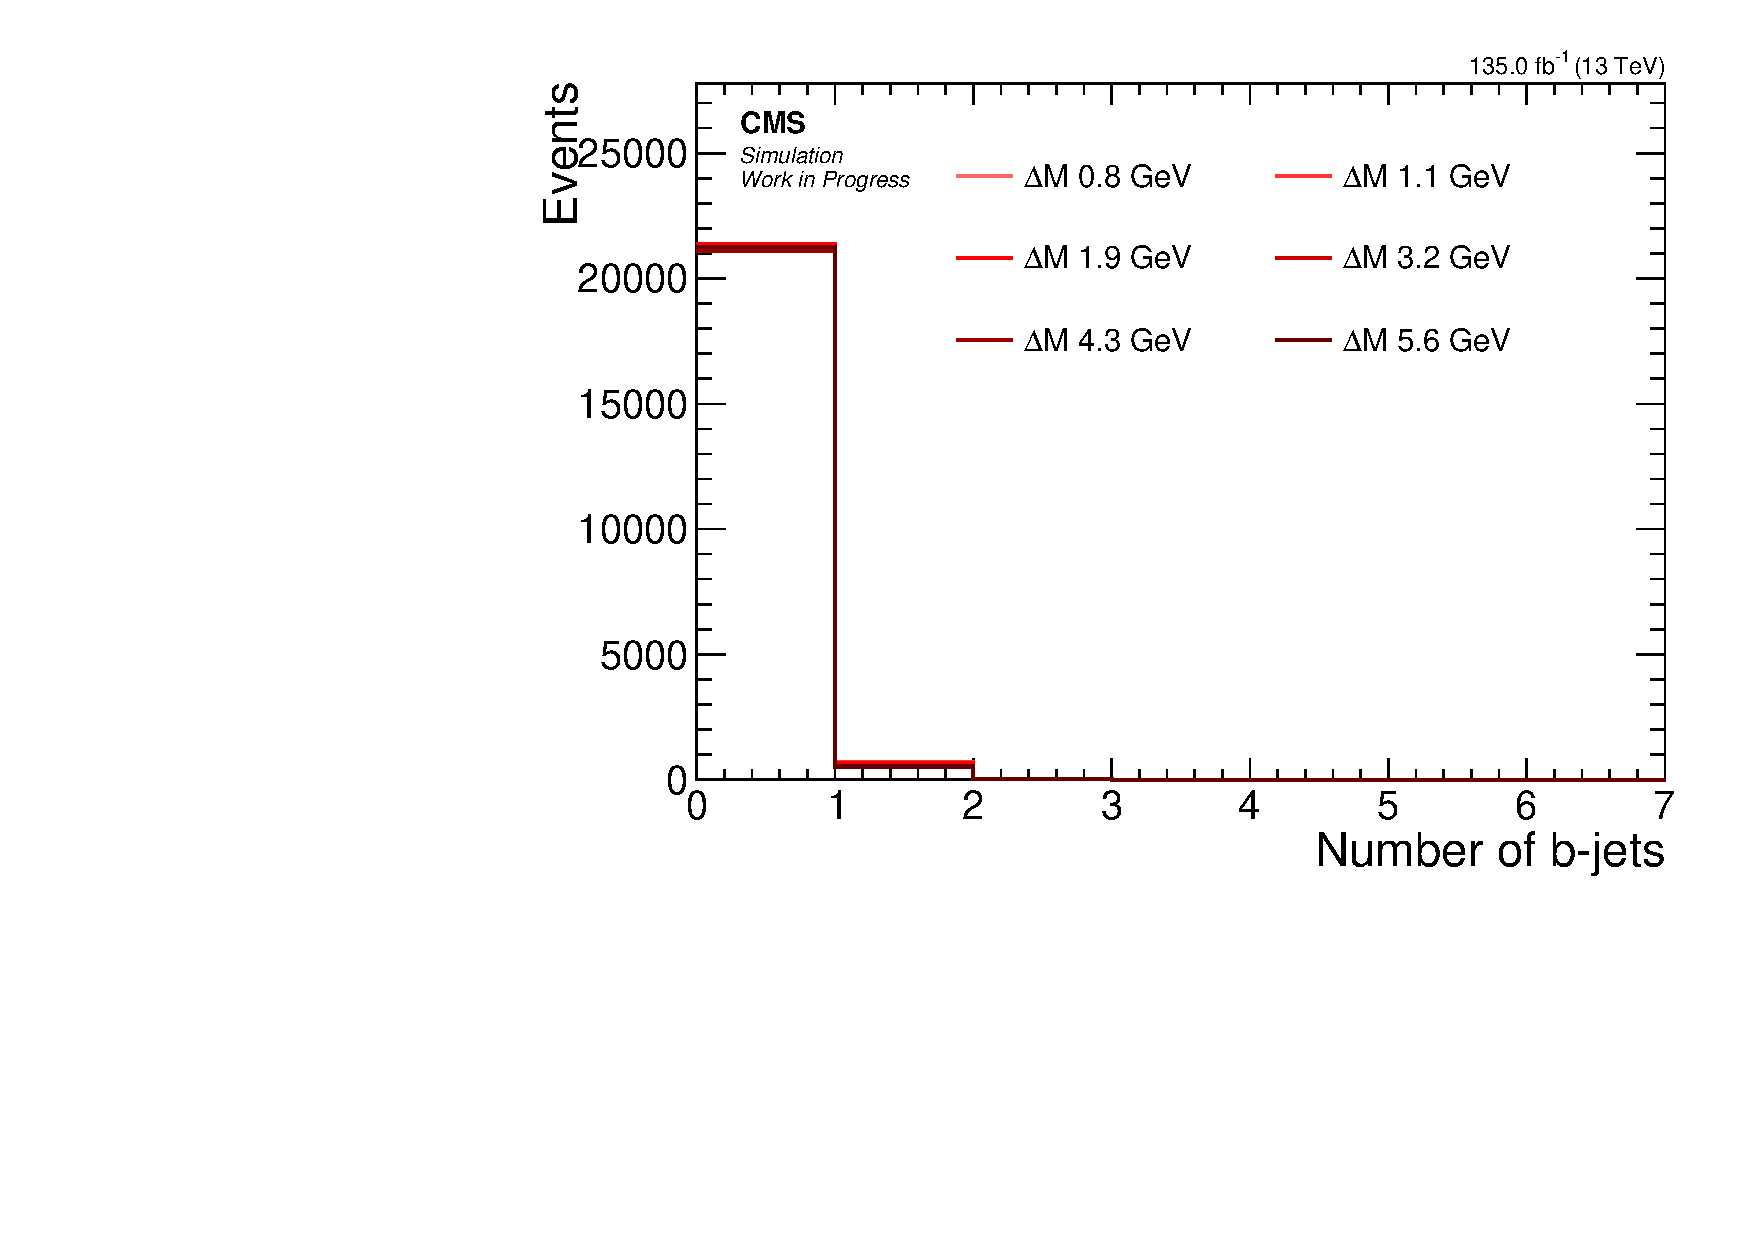
\includegraphics[width=0.48\linewidth]{plots/signal_common_distributions_fixed_mu/none_BTagsDeepMedium.pdf} \,
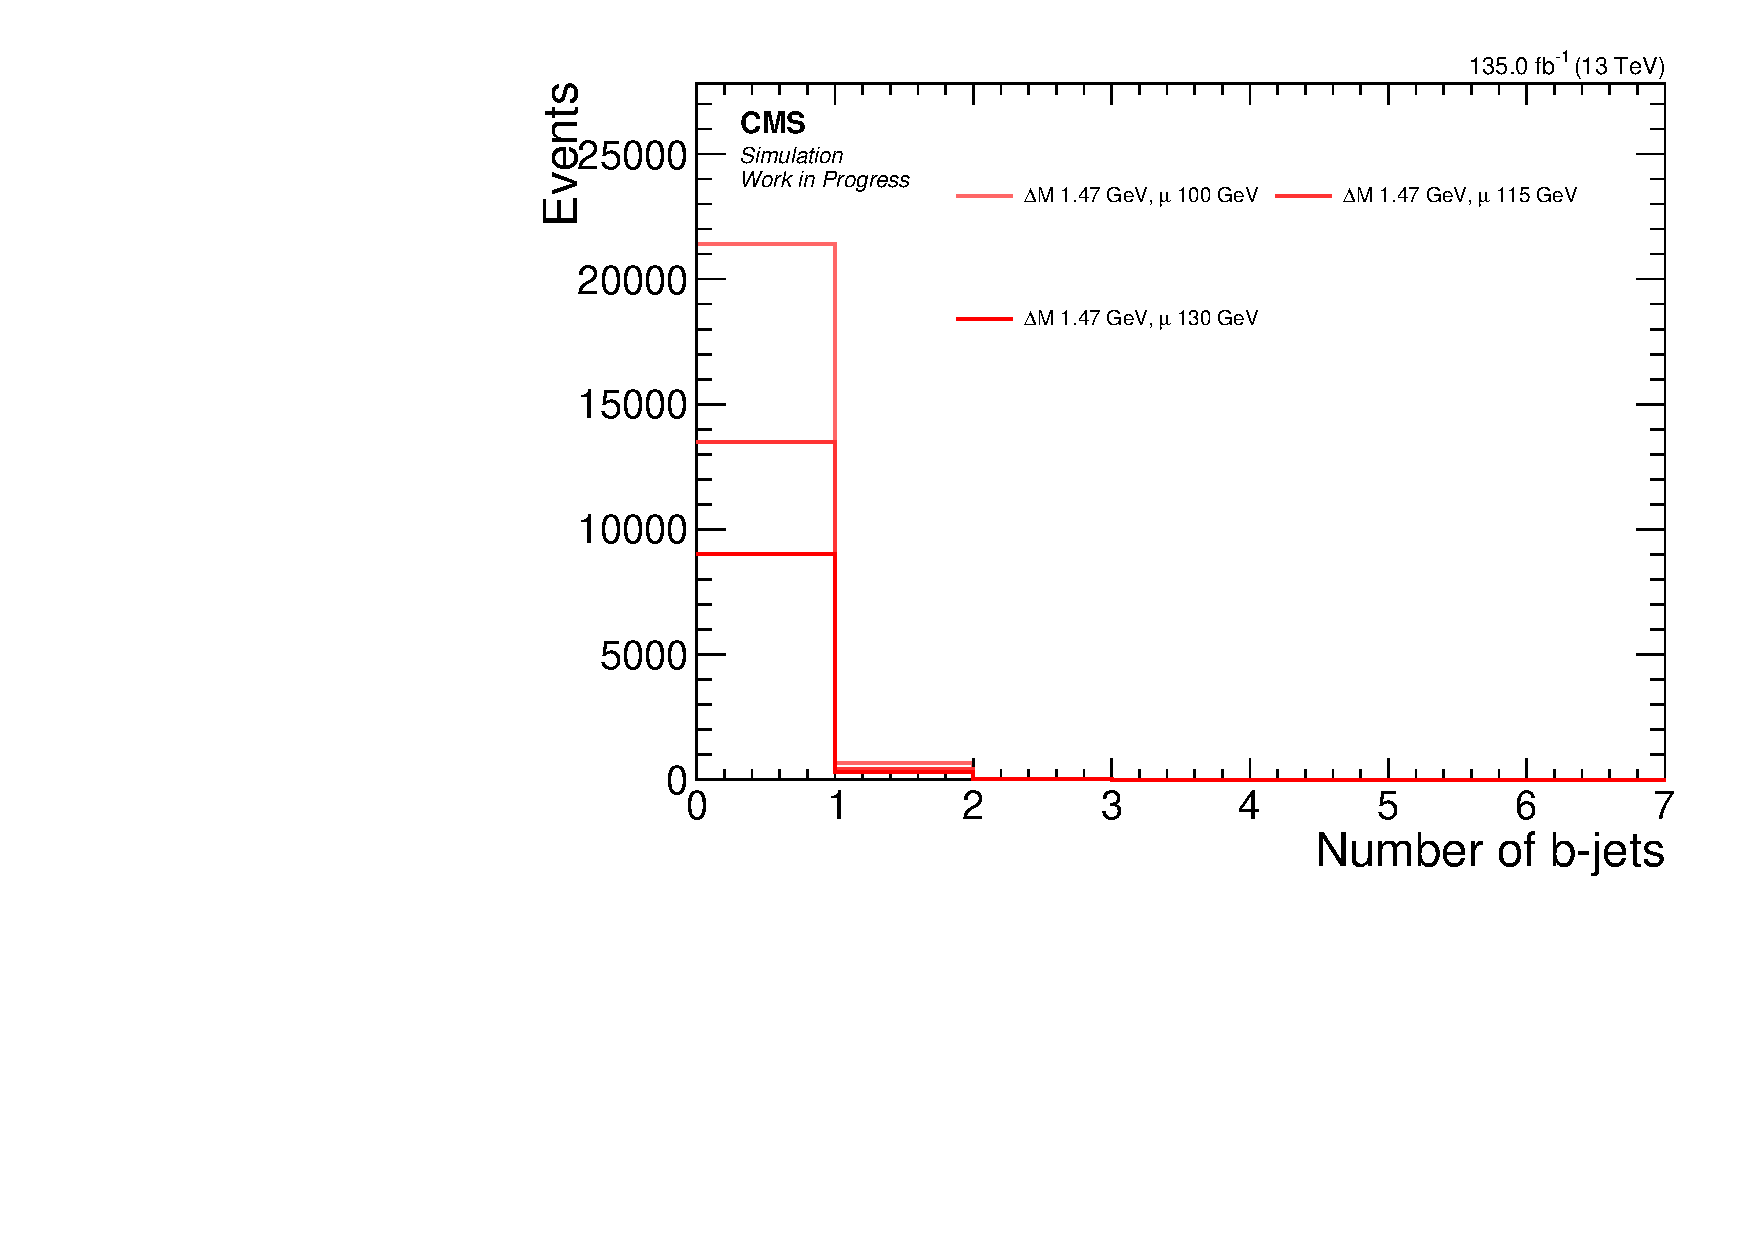
\includegraphics[width=0.48\linewidth]{plots/signal_common_distributions_fixed_dm/none_BTagsDeepMedium.pdf}  \\
\caption[Signal \emph{number of b-tagged jets} distributions]{ Signal distributions for \emph{number of b-tagged jets} comparing various $\dm$ with a fixed higgsino parameter $\mu=100\GeV$ (left), and comparing various higgsino parameters $\mu$ with fixed $\dm=1.47\GeV$ (right).}
\label{fig:signal-bjets}
\end{figure}

As an \gls{isr} jet is required in the event, it is expected that the \gls{met} and the \gls{mht} will be directed in the opposite direction of the jet, or at an angle close to $\pi$. This feature will not be observed in events with multiple jets in the \gls{sm} background, such as those arising from \gls{qcd}. To reduce the \gls{qcd} background, a requirement of $\mindphimhtjets > 0.4$ is imposed.

\begin{figure}[!htb]
\centering
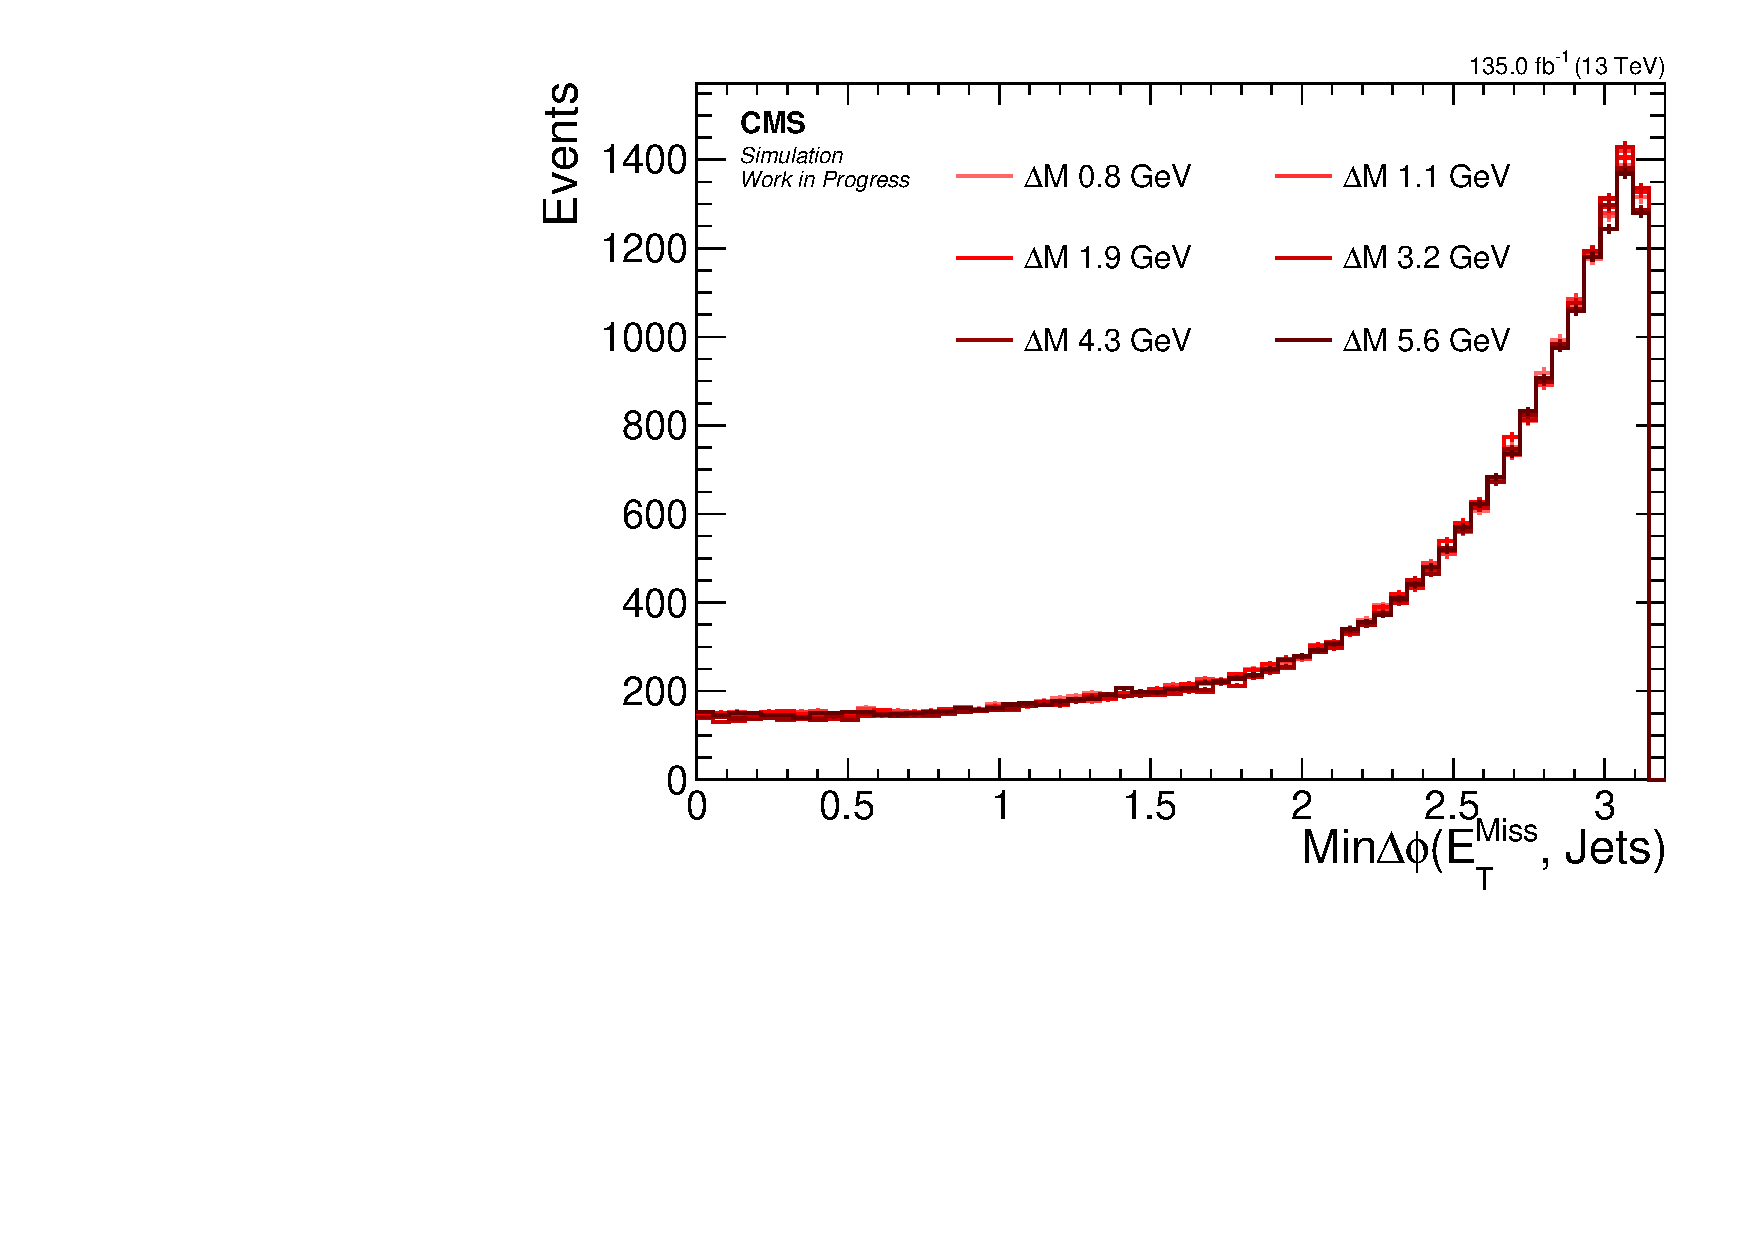
\includegraphics[width=0.48\linewidth]{plots/signal_common_distributions_fixed_mu/none_MinDeltaPhiMetJets.pdf} \,
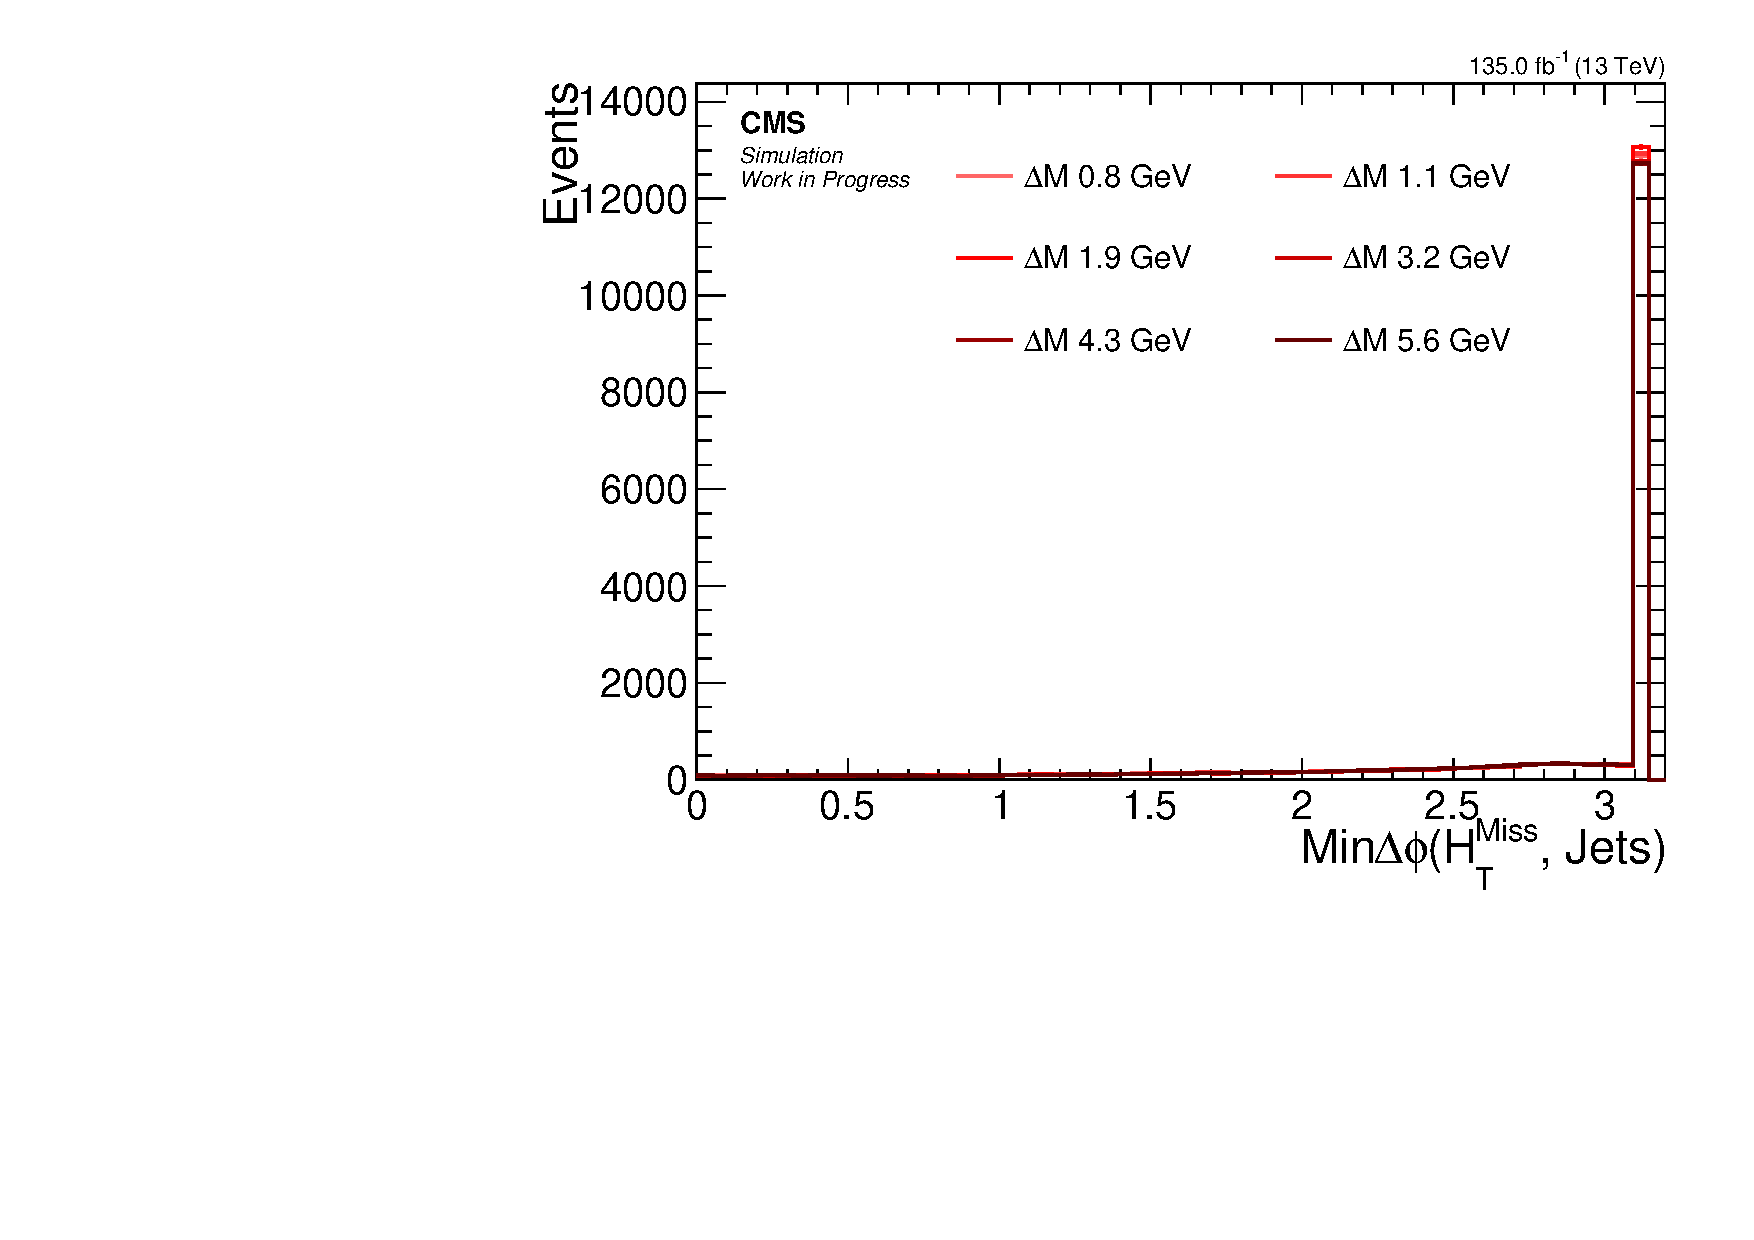
\includegraphics[width=0.48\linewidth]{plots/signal_common_distributions_fixed_mu/none_MinDeltaPhiMhtJets.pdf}  \\
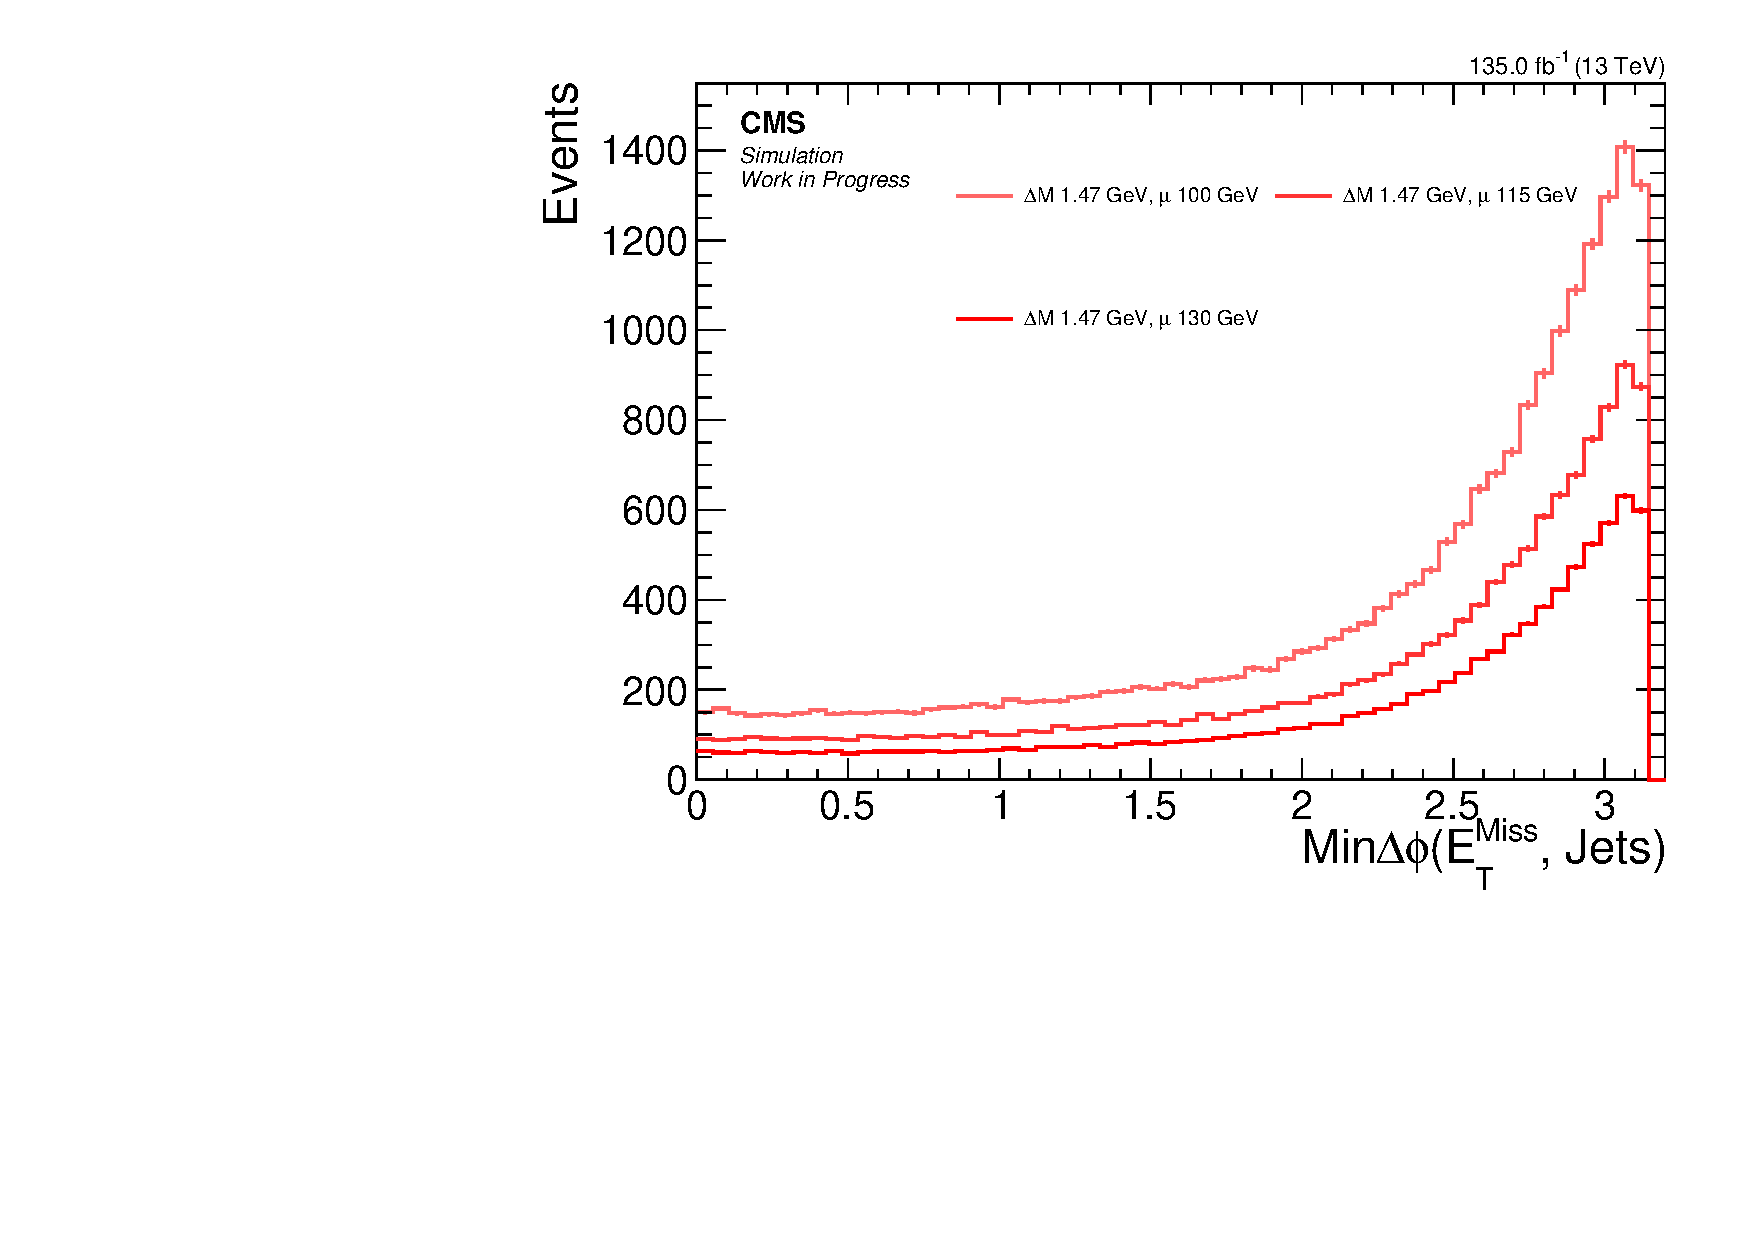
\includegraphics[width=0.48\linewidth]{plots/signal_common_distributions_fixed_dm/none_MinDeltaPhiMetJets.pdf} \,
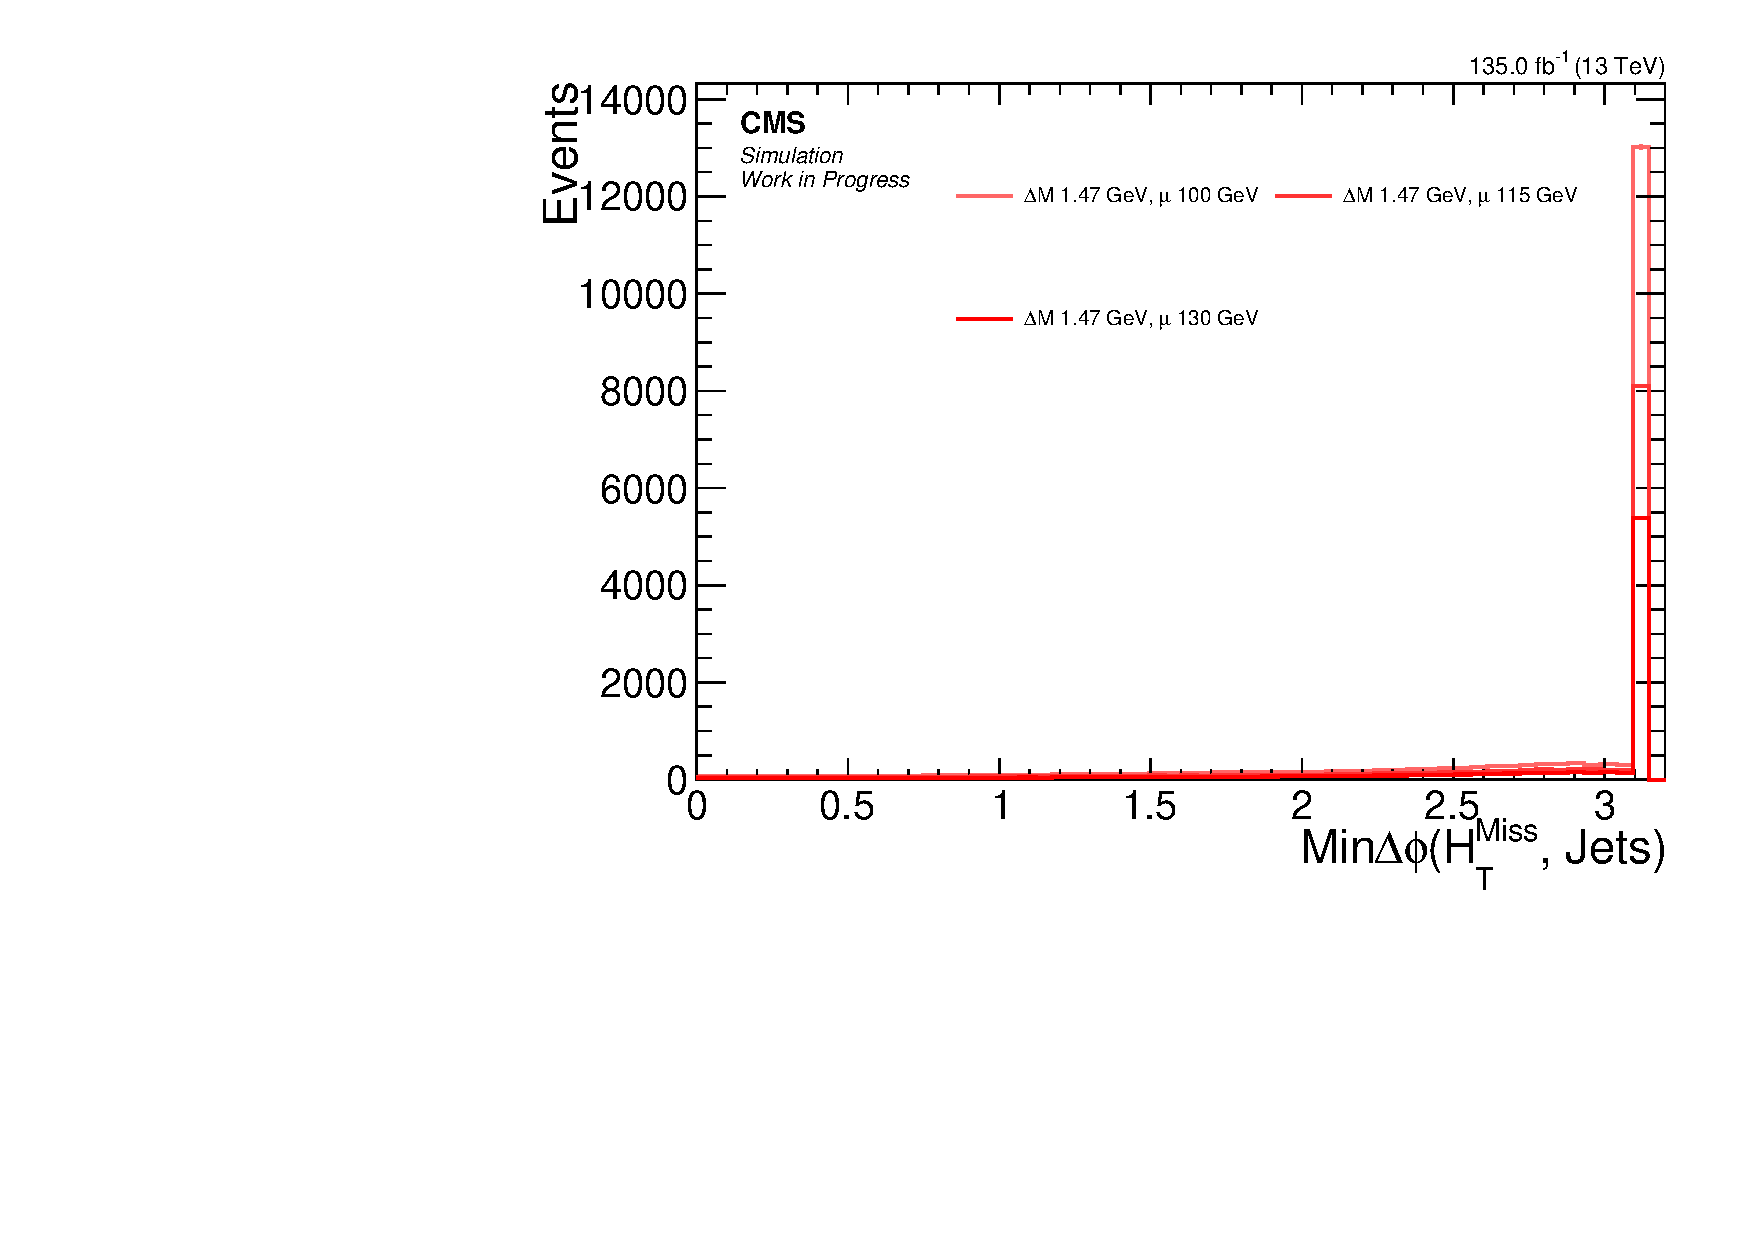
\includegraphics[width=0.48\linewidth]{plots/signal_common_distributions_fixed_dm/none_MinDeltaPhiMhtJets.pdf}  \\
\caption[Signal $\mindphimetjets$ and $\mindphimhtjets$ distributions]{ Signal distributions for \mindphimetjets (left) and \mindphimhtjets (right) comparing various $\dm$ with a fixed higgsino parameter $\mu=100\GeV$ (upper), and comparing various higgsino parameters $\mu$ with fixed $\dm=1.47\GeV$ (lower).}
\label{fig:signal-min-deltaphi-met-mht}
\end{figure}

\subsection{Base selection}

The section is recapped by summarizing the base selection of the analysis. The base selection, also known interchangeably as the preselection, is applied to all analysis categories. It ls listed in Table~\ref{tab:base-selection}.

\begin{table}[!htb]
	\centering
	\label{tab:base-selection}
		\caption{Base selection applied to all analysis categories}
		%\vspace{1mm}
			\begin{tabular}{lc} \hline
			Variable & Value \\ \hline
			$\mht \left[\GeV\right]$ & $\geq220$ \\
			$\njets \left( \pt \geq 30\GeV\, \mathrm{and}\, \abs{\eta} < 2.4 \right)$ & $\geq 1$\\
			$\nbjets \left( \pt \geq 30\GeV\, \mathrm{and}\, \abs{\eta} < 2.4 \right)$ & 0 \\
			$\mindphimhtjets$ & $ > 0.4$ \\ \hline
			\end{tabular}
\end{table}

\clearpage
\subsection{Dilepton kinematics}

Kinematic distributions have been examined so far, with the leptons in the event ignored. However, the dilepton system contains the most distinctive features of the signal. To fully understand the unique phase space of the dilepton system, generator level distributions are examined first, followed by an exploration of the effects of reconstruction on those observables. Since the dimuon category is the most sensitive due to its lower threshold on the leptons' transverse momentum, events with two electrons are excluded from the following sections, focusing on the muons. The kinematics change dramatically as a function of \dm. In contrast, the higgsino parameter $\mu$ effects almost only the overall normalization due to the different production cross section. Therefore, the higgsino parameter is set to $\mu=100\GeV$ in the following sections, with the \dm varied.

\subsubsection{Lepton $\eta$ and transverse momentum \gls{pt}}
\label{sec:muon-eta-pt}

The signal acceptance and sensitivity are significantly impacted by the accessible thresholds of the transverse momentum \gls{pt} distribution of the muons. The muon reconstruction process and details are discussed in Section~\ref{id-muons}. The selection applied to the muons in this analysis is described in Section~\ref{sec:muon-selection} and referred to as \emph{analysis selection}. This section aims to examine the importance of the \gls{pt} on the signal and its dilepton kinematic distributions.

The generator level distribution of \gls{pt}, or the so-called \emph{truth} distributions, which do not exhibit any detector or reconstruction features, are examined first. The reconstructed distribution is then compared with the generator level distribution in Figure~\ref{fig:signal-muons-pt}. 

\begin{figure}[!htb]
\centering
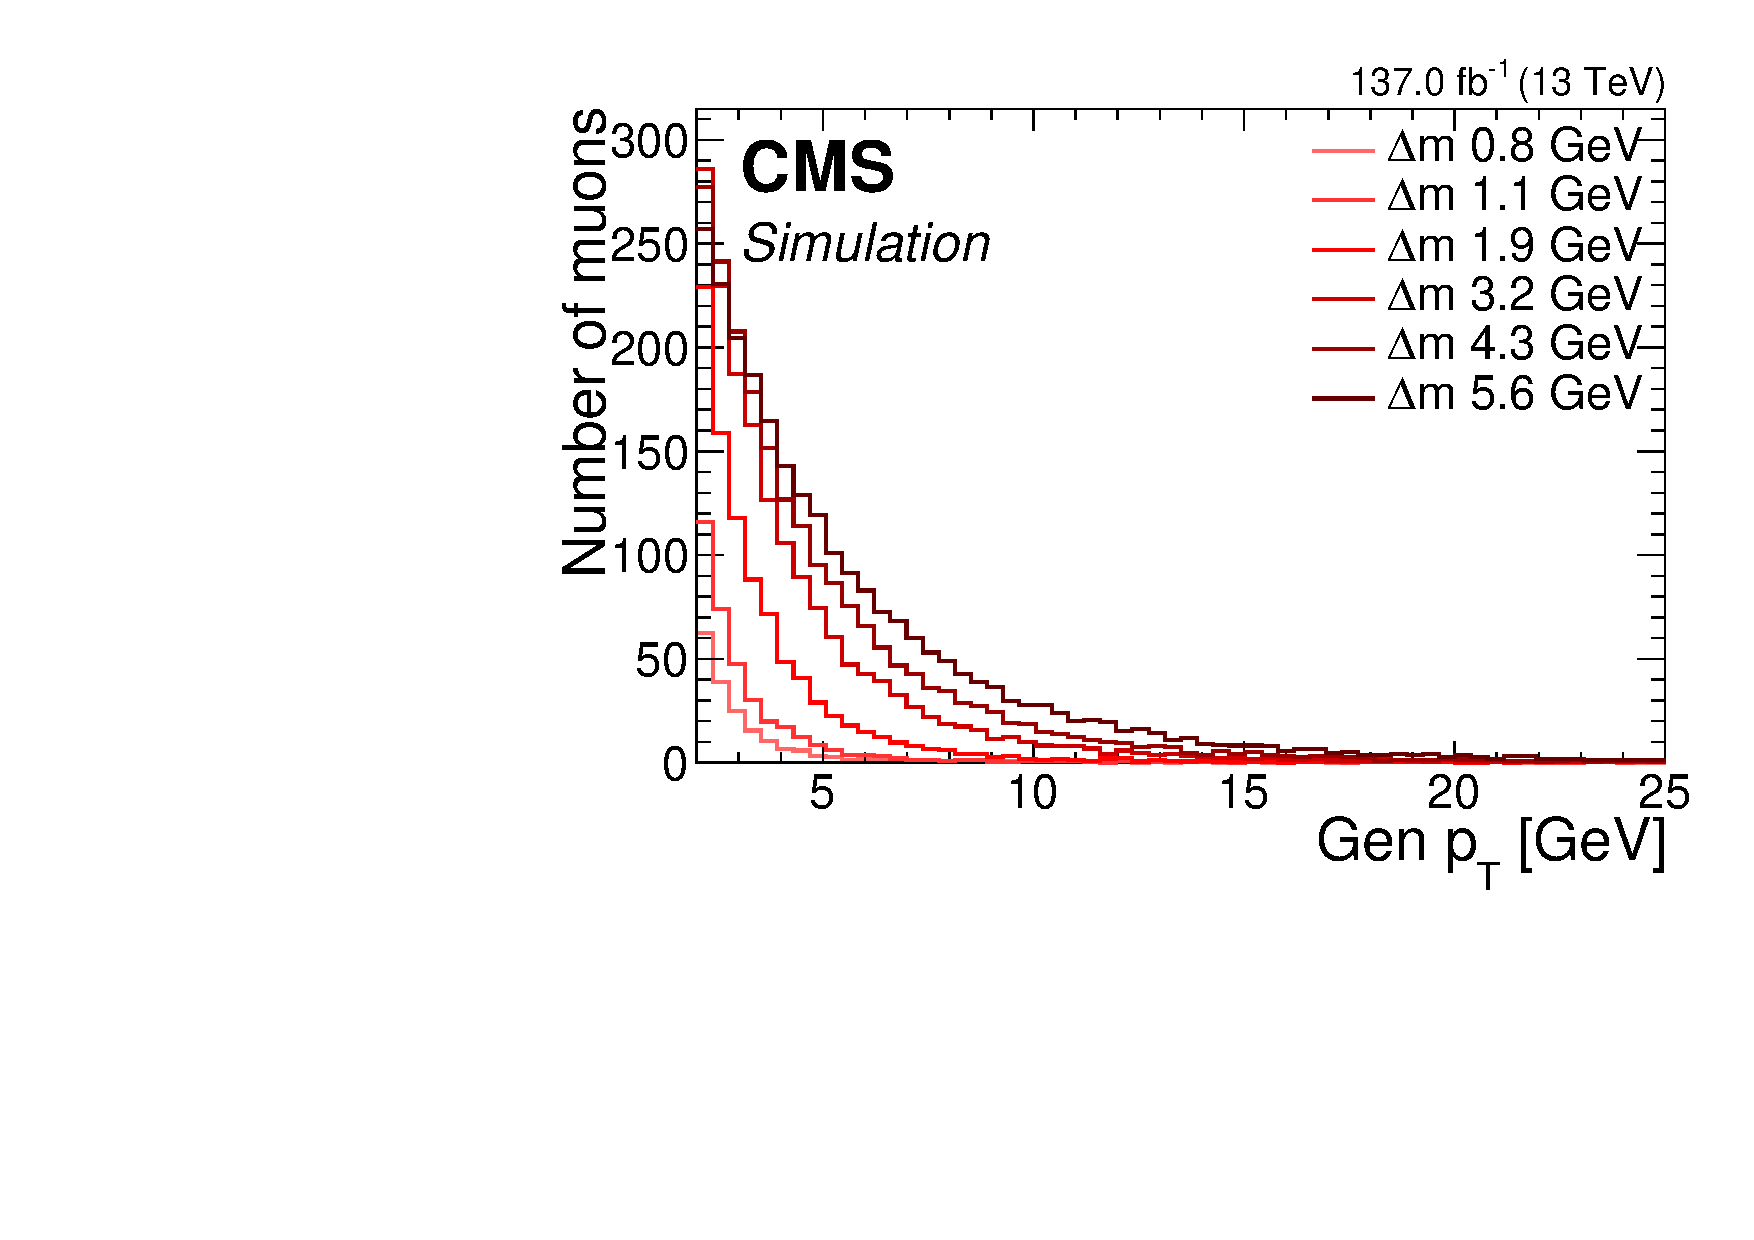
\includegraphics[width=0.32\linewidth]{plots/signal_muons_gen/none_Muons_pt.pdf} \,
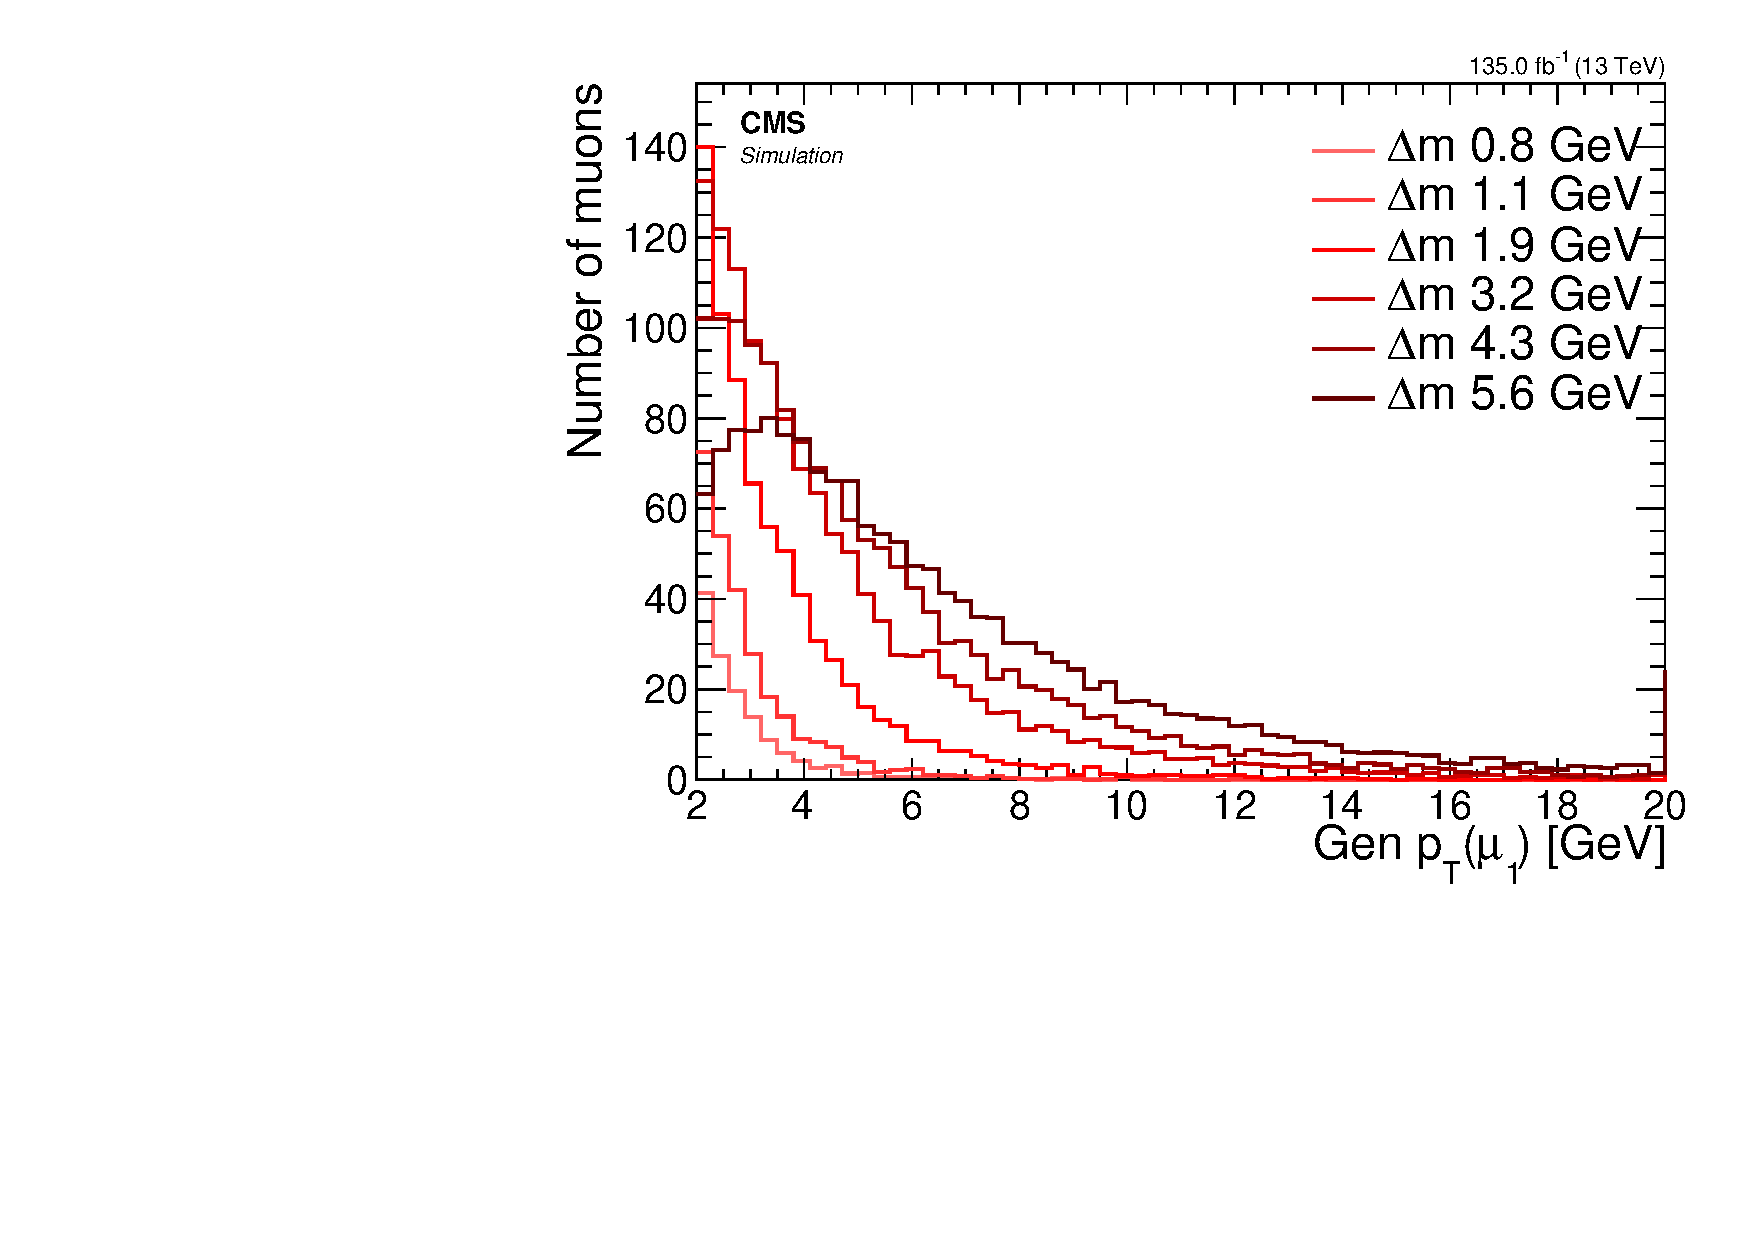
\includegraphics[width=0.32\linewidth]{plots/signal_muons_gen/none_Muons_m1_pt.pdf}  \,
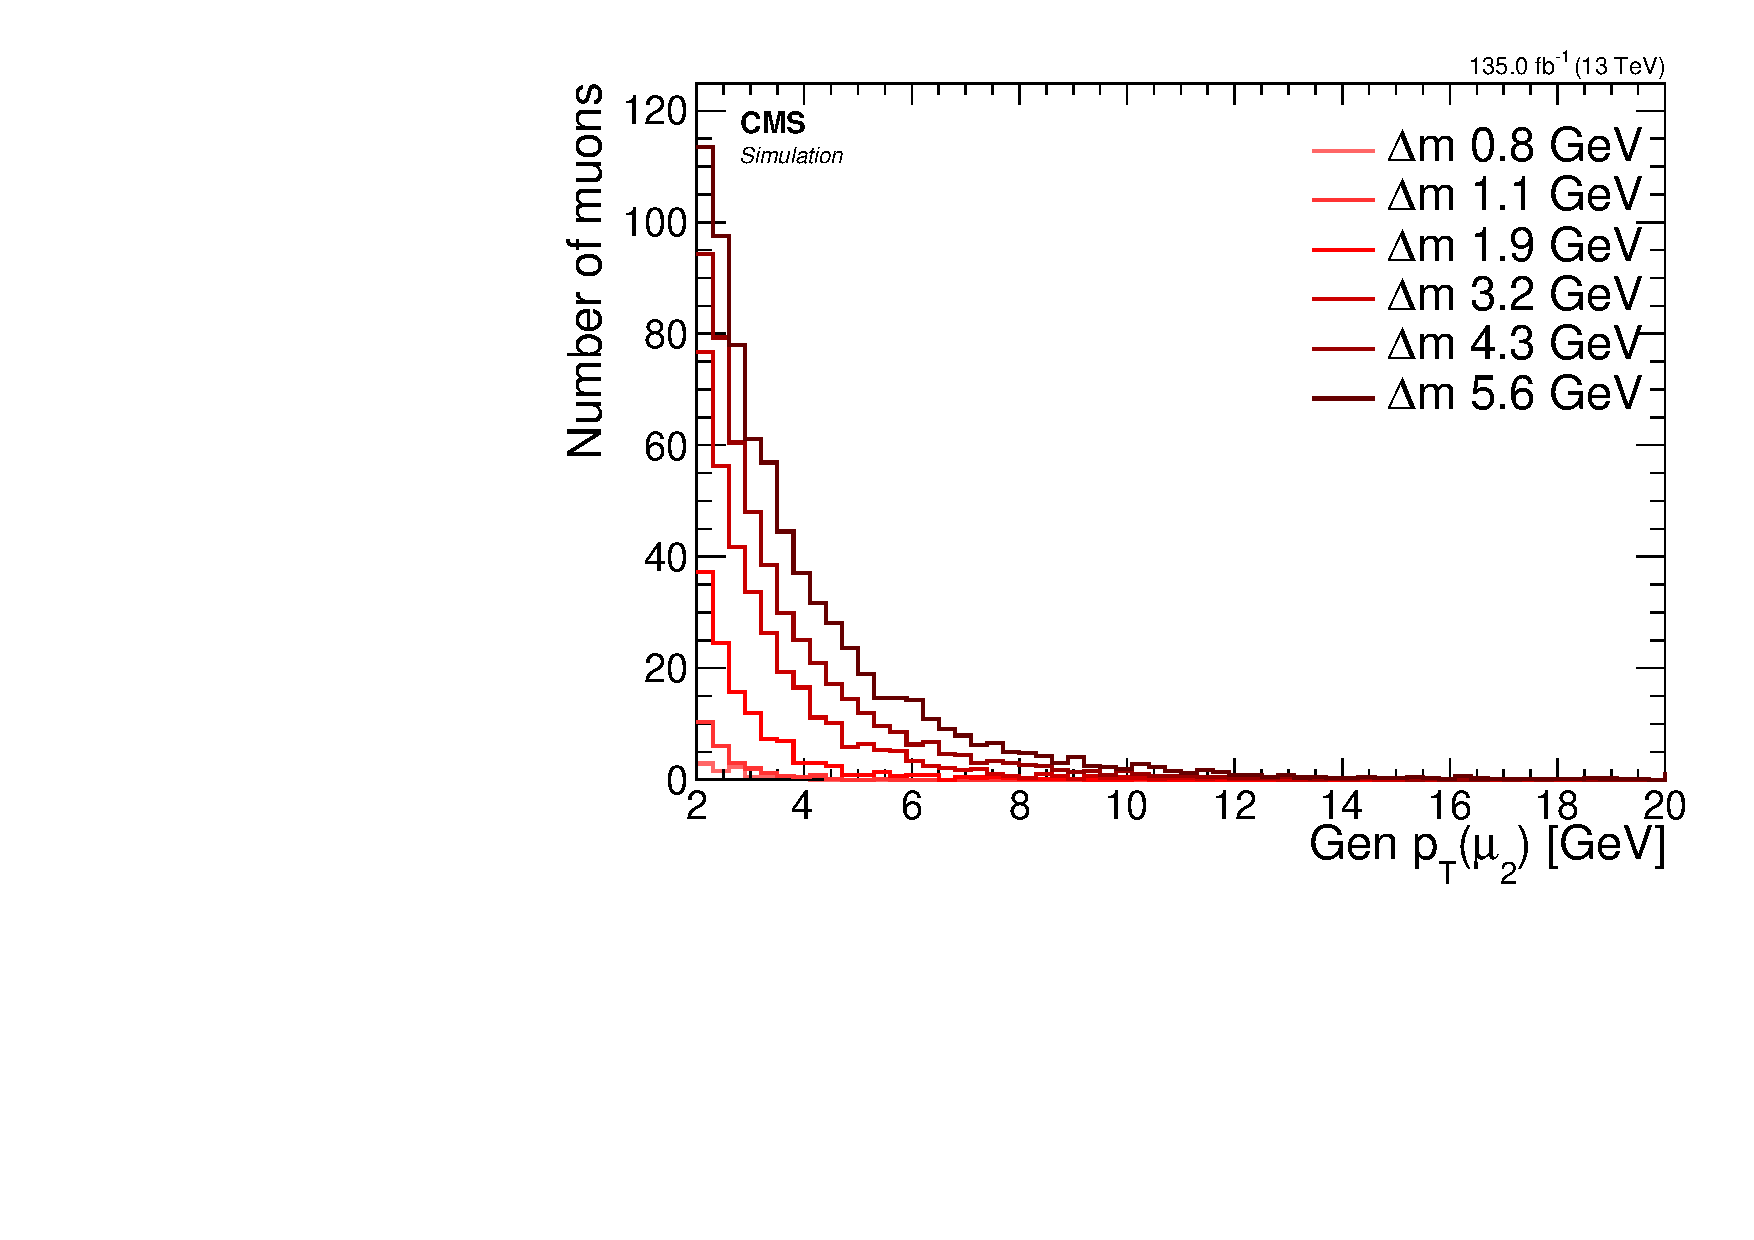
\includegraphics[width=0.32\linewidth]{plots/signal_muons_gen/none_Muons_m2_pt.pdf} \\
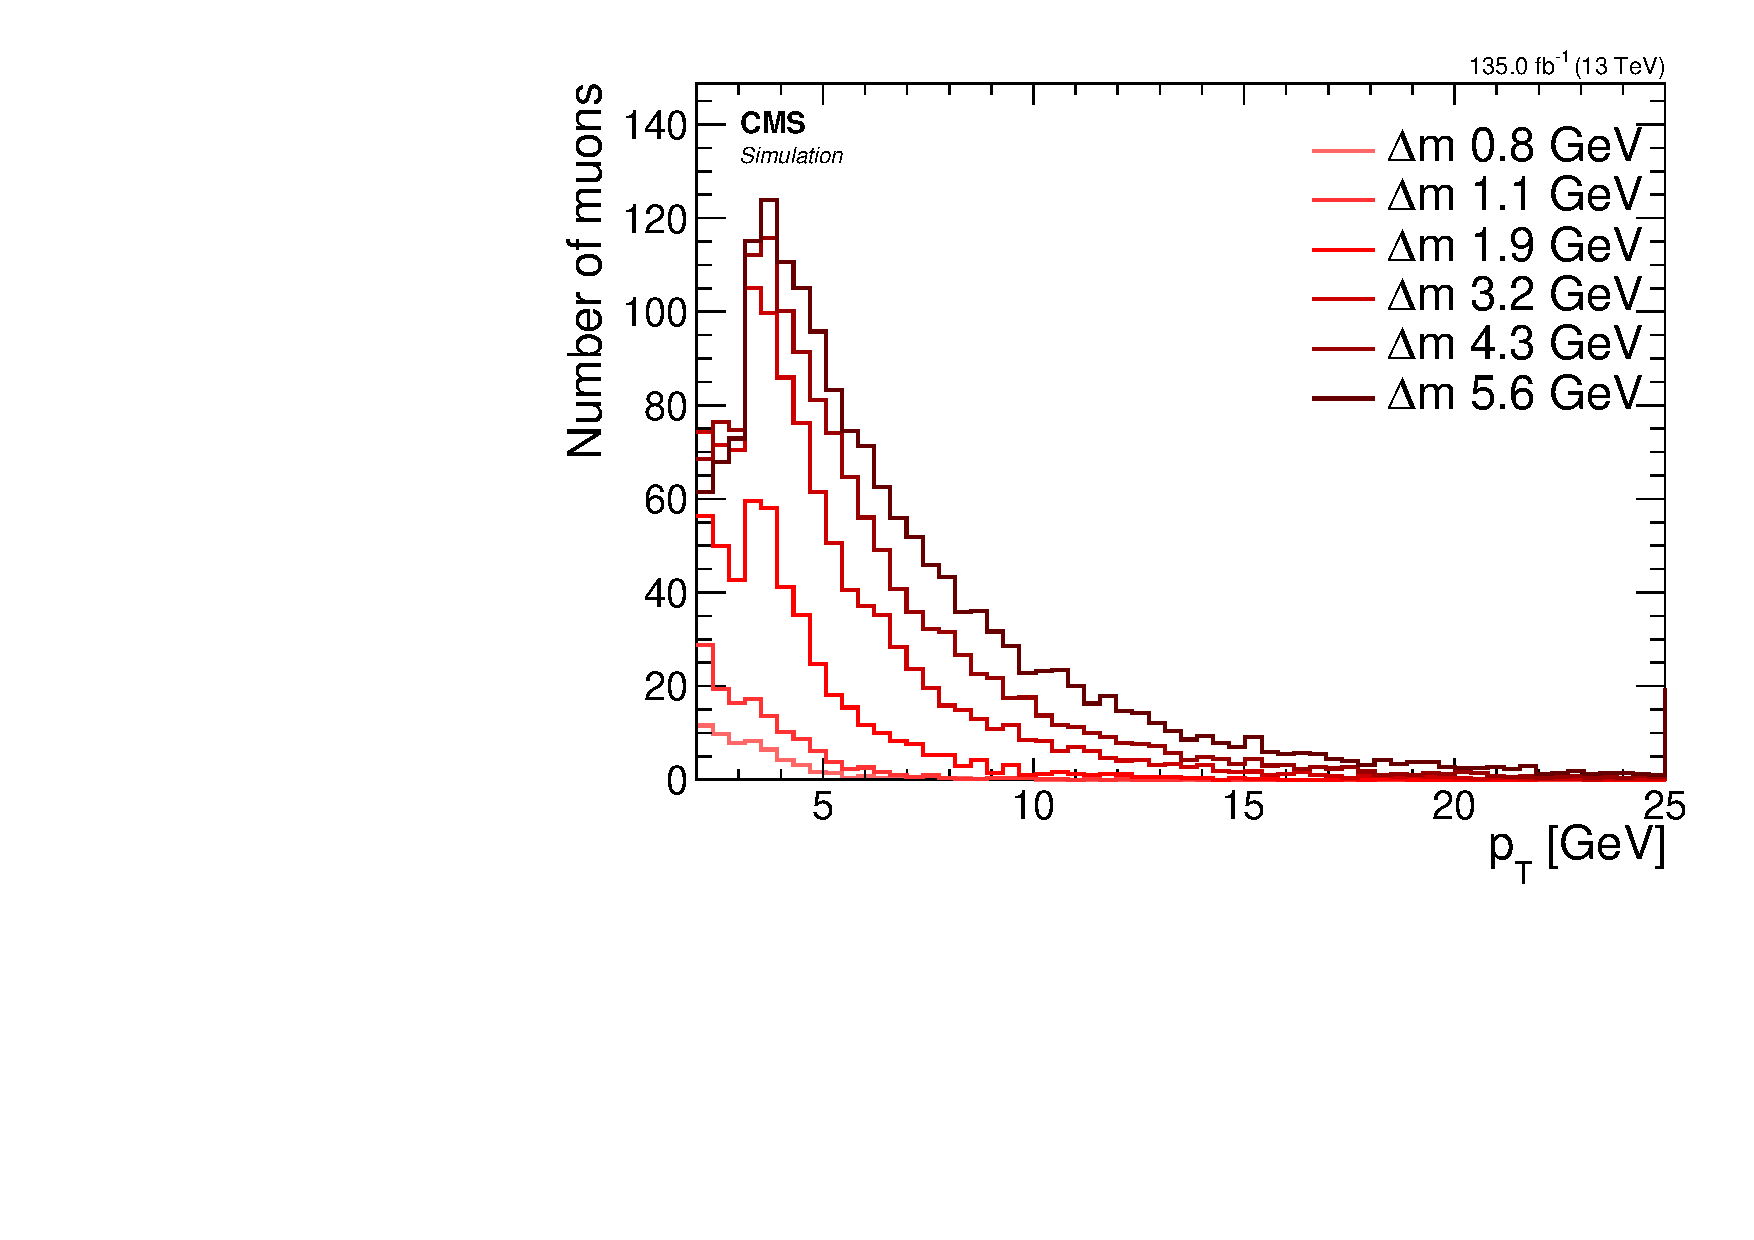
\includegraphics[width=0.32\linewidth]{plots/signal_muons/none_Muons_pt.pdf} \,
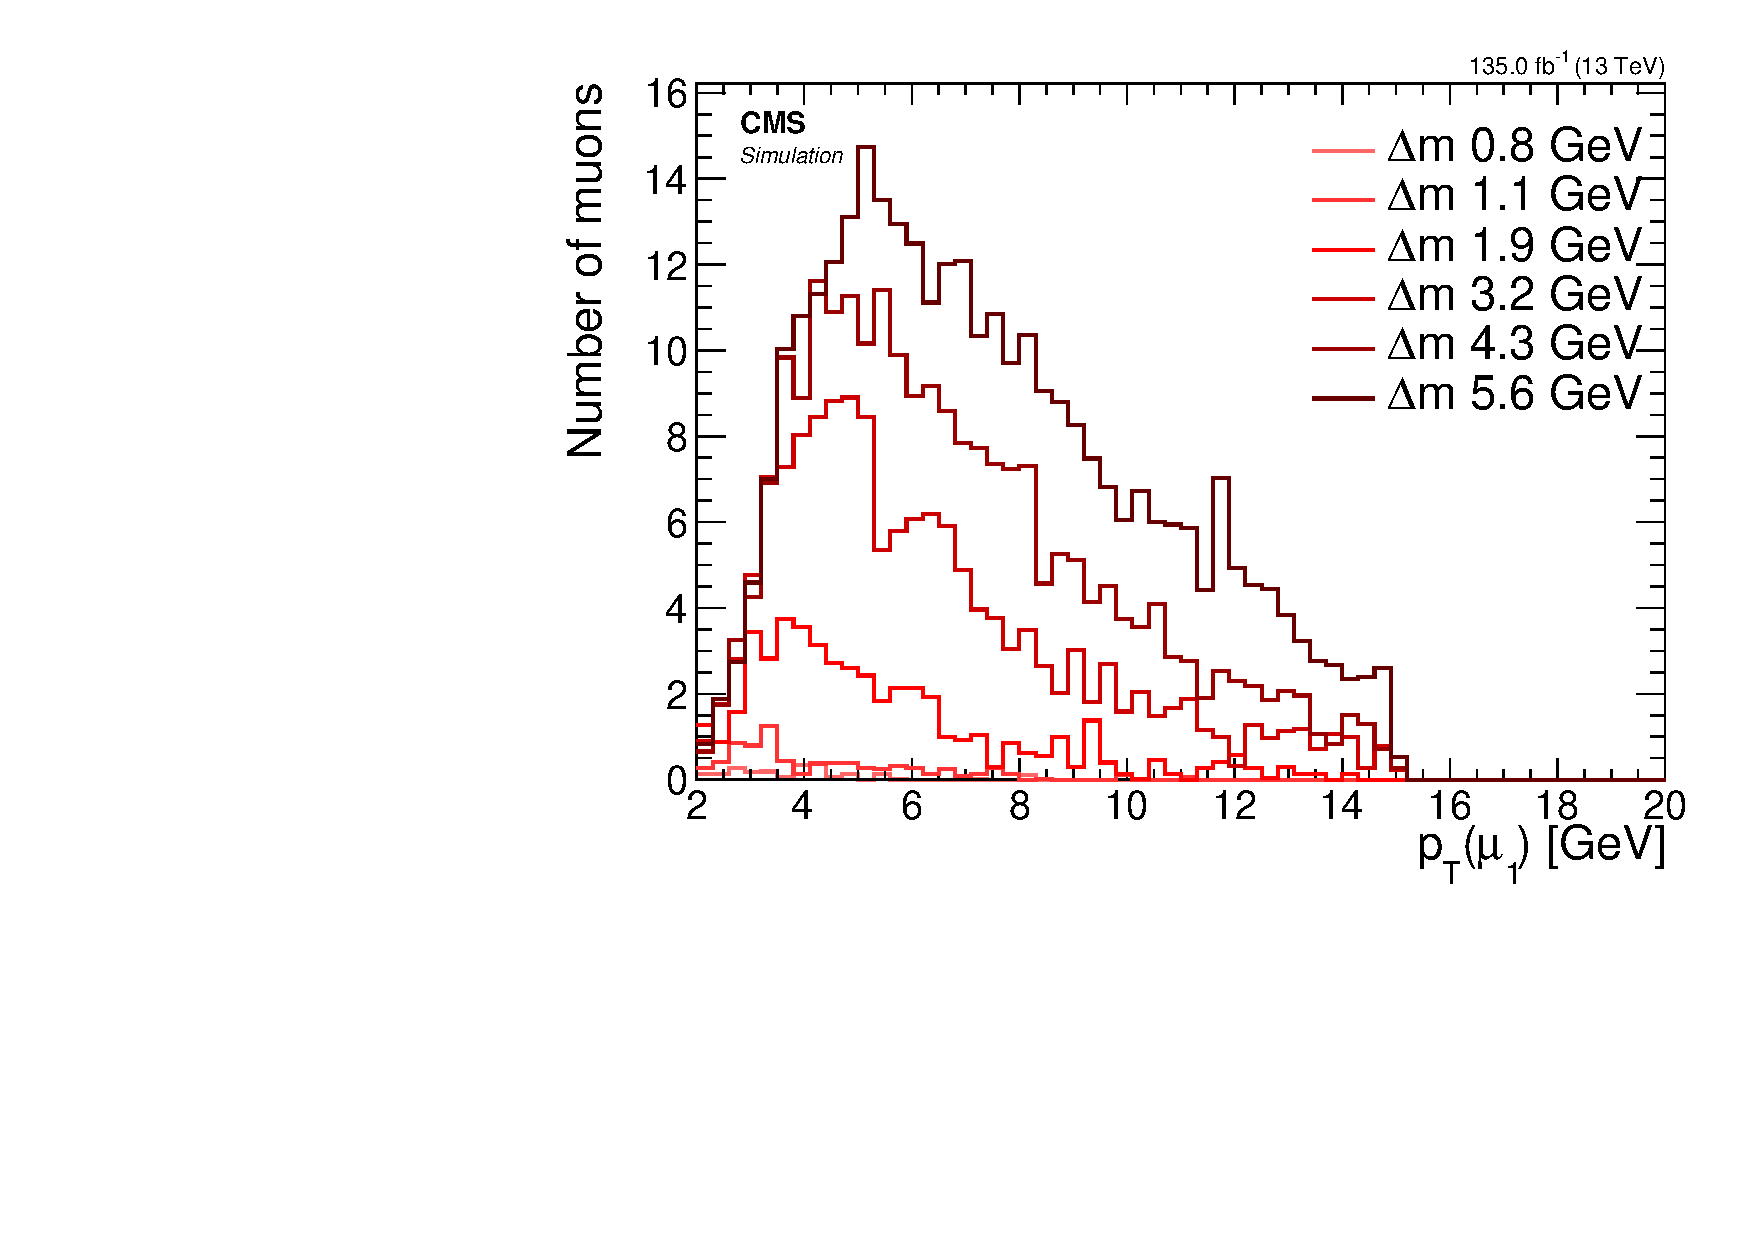
\includegraphics[width=0.32\linewidth]{plots/signal_muons/none_Muons_m1_pt.pdf}  \,
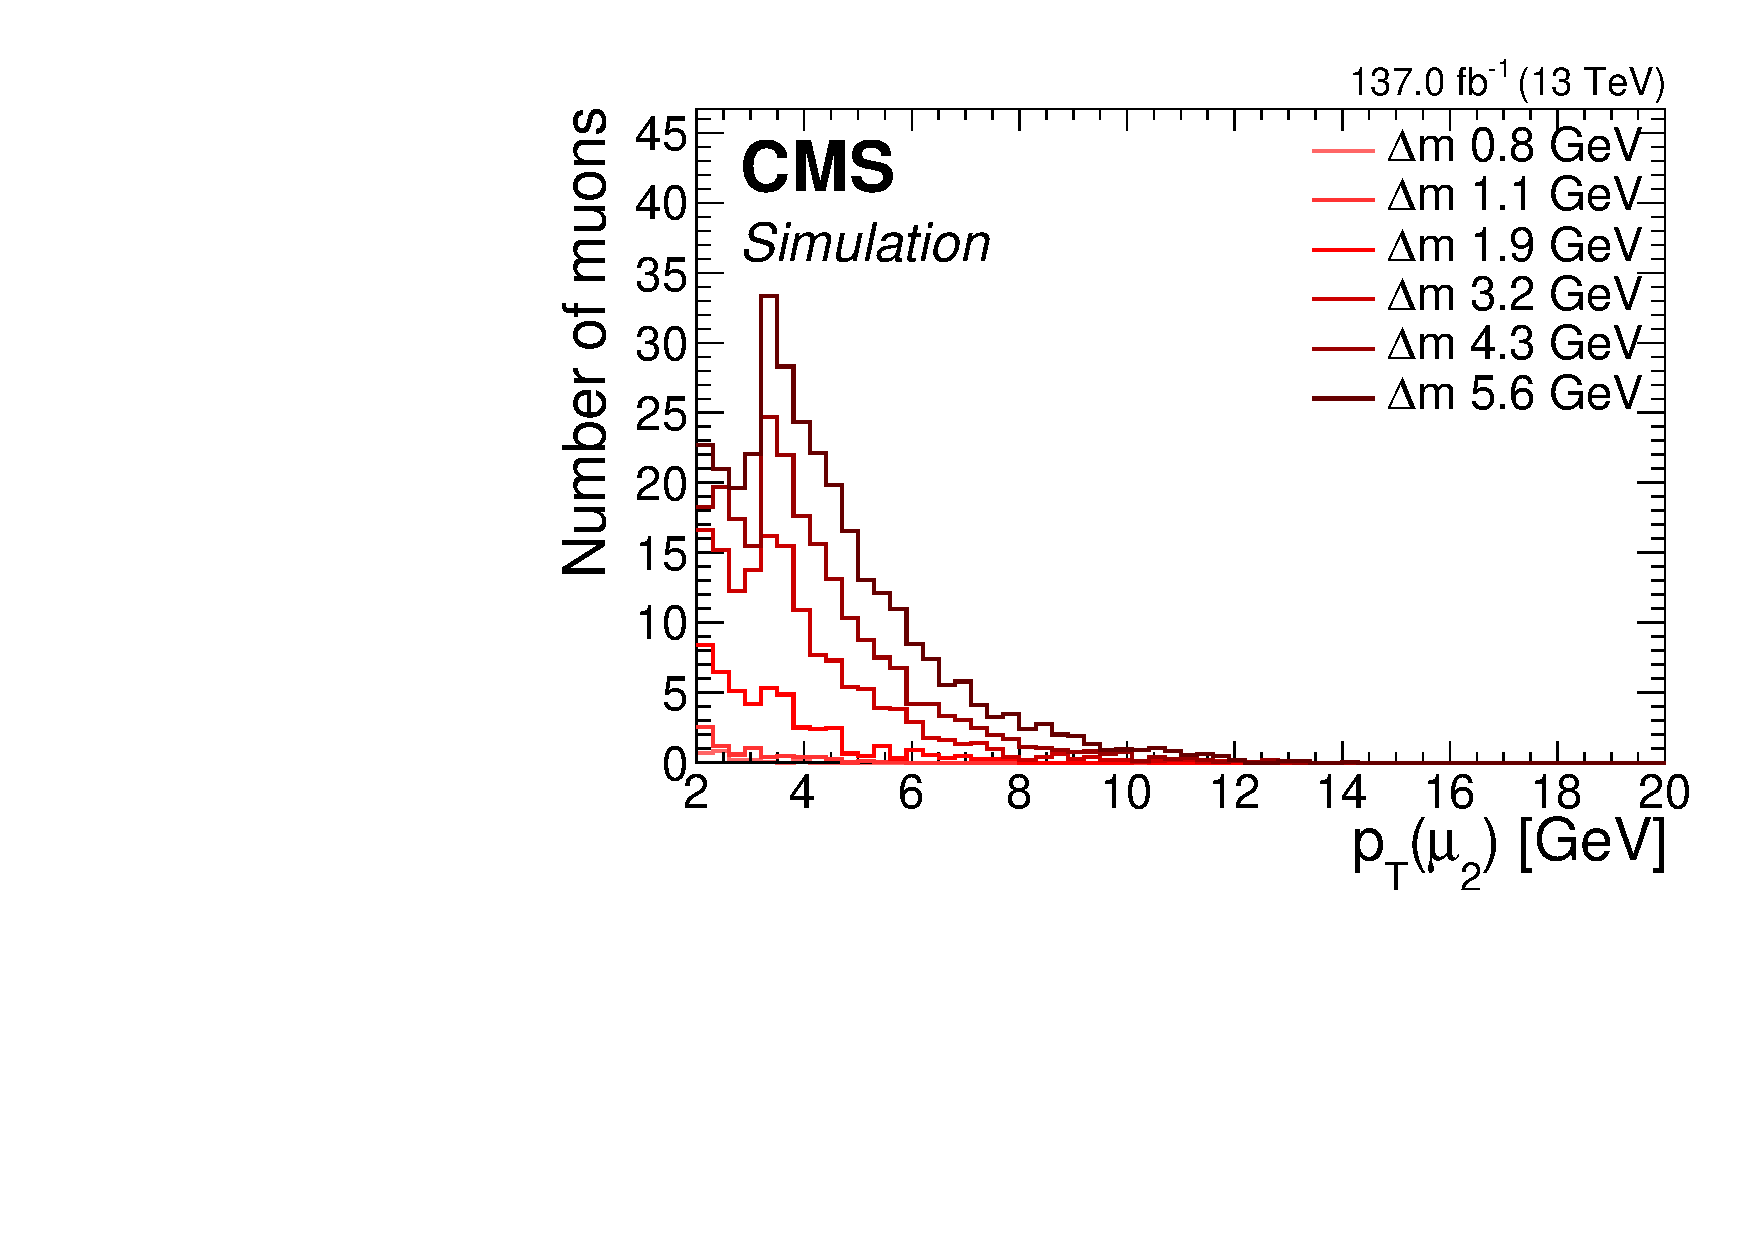
\includegraphics[width=0.32\linewidth]{plots/signal_muons/none_Muons_m2_pt.pdf} \\
\caption[Signal \pt distributions]{ Signal \pt distributions for inclusive (left), leading muon $\mu_1$ (middle),  subleading muon $\mu_2$ (right) at generator level (top) and reconstruction level passing analysis selection (bottom). }
\label{fig:signal-muons-pt}
\end{figure}

When comparing the generator level to the reconstruction level of the inclusive \pt distribution, it becomes apparent that a reshaping occurs around $3 \GeV$. A significant proportion of the generated muons with $\pt<3\GeV$ is lost in the reconstruction process. The subleading muon \pt distribution at the reconstruction level has a camel shape, whereby the efficiency drops below a \pt of $3\GeV$ and is only partially regained at $\pt<3\GeV$. This effect is due to the detector and is more clearly visible when splitting the \pt distribution into a barrel ($\abs{\eta} < 1.2$) and encaps ($\abs{\eta} \geq 1.2$) portions, as shown in Figure~\ref{fig:signal-pt-barrel-endcaps}.

\begin{figure}[!htb]
\centering
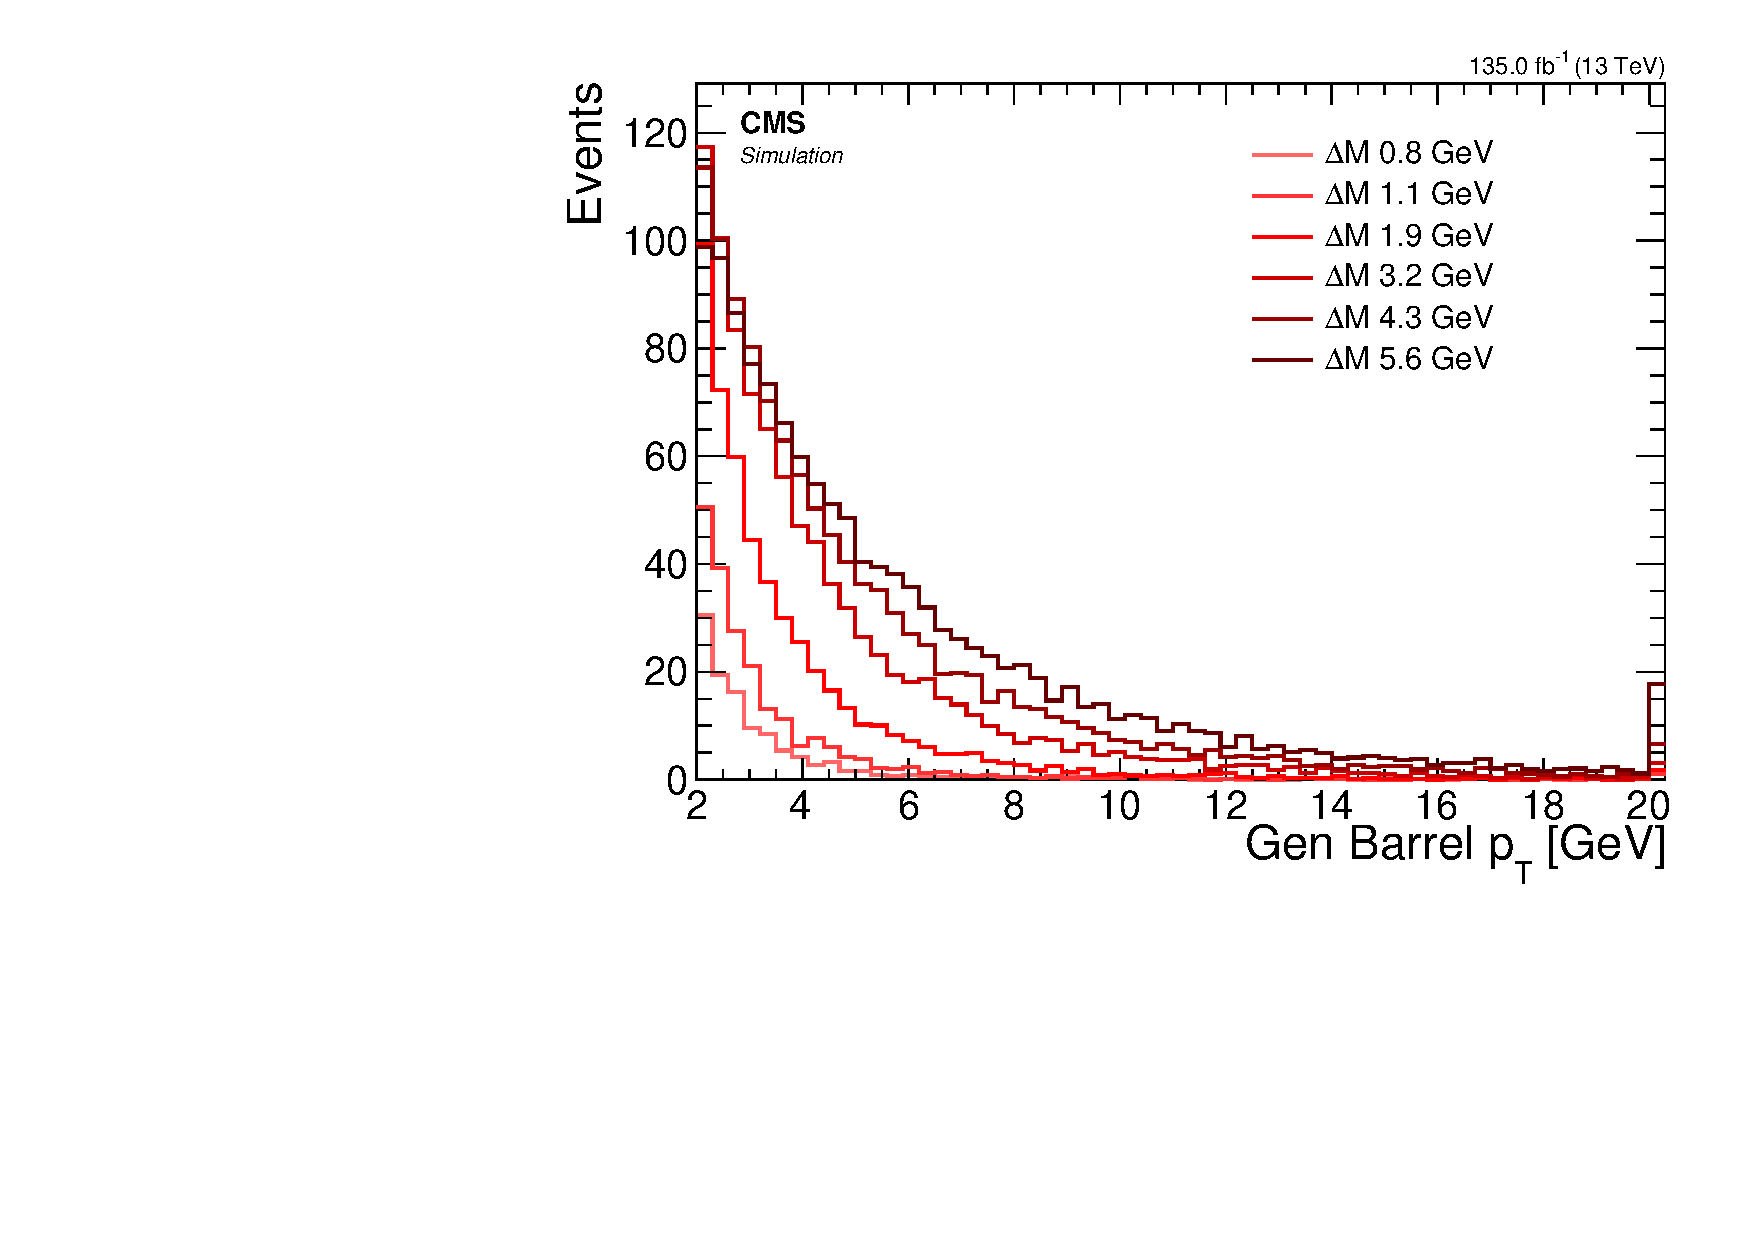
\includegraphics[width=0.48\linewidth]{plots/signal_muons_gen/none_Muons_pt_barrel.pdf} \,
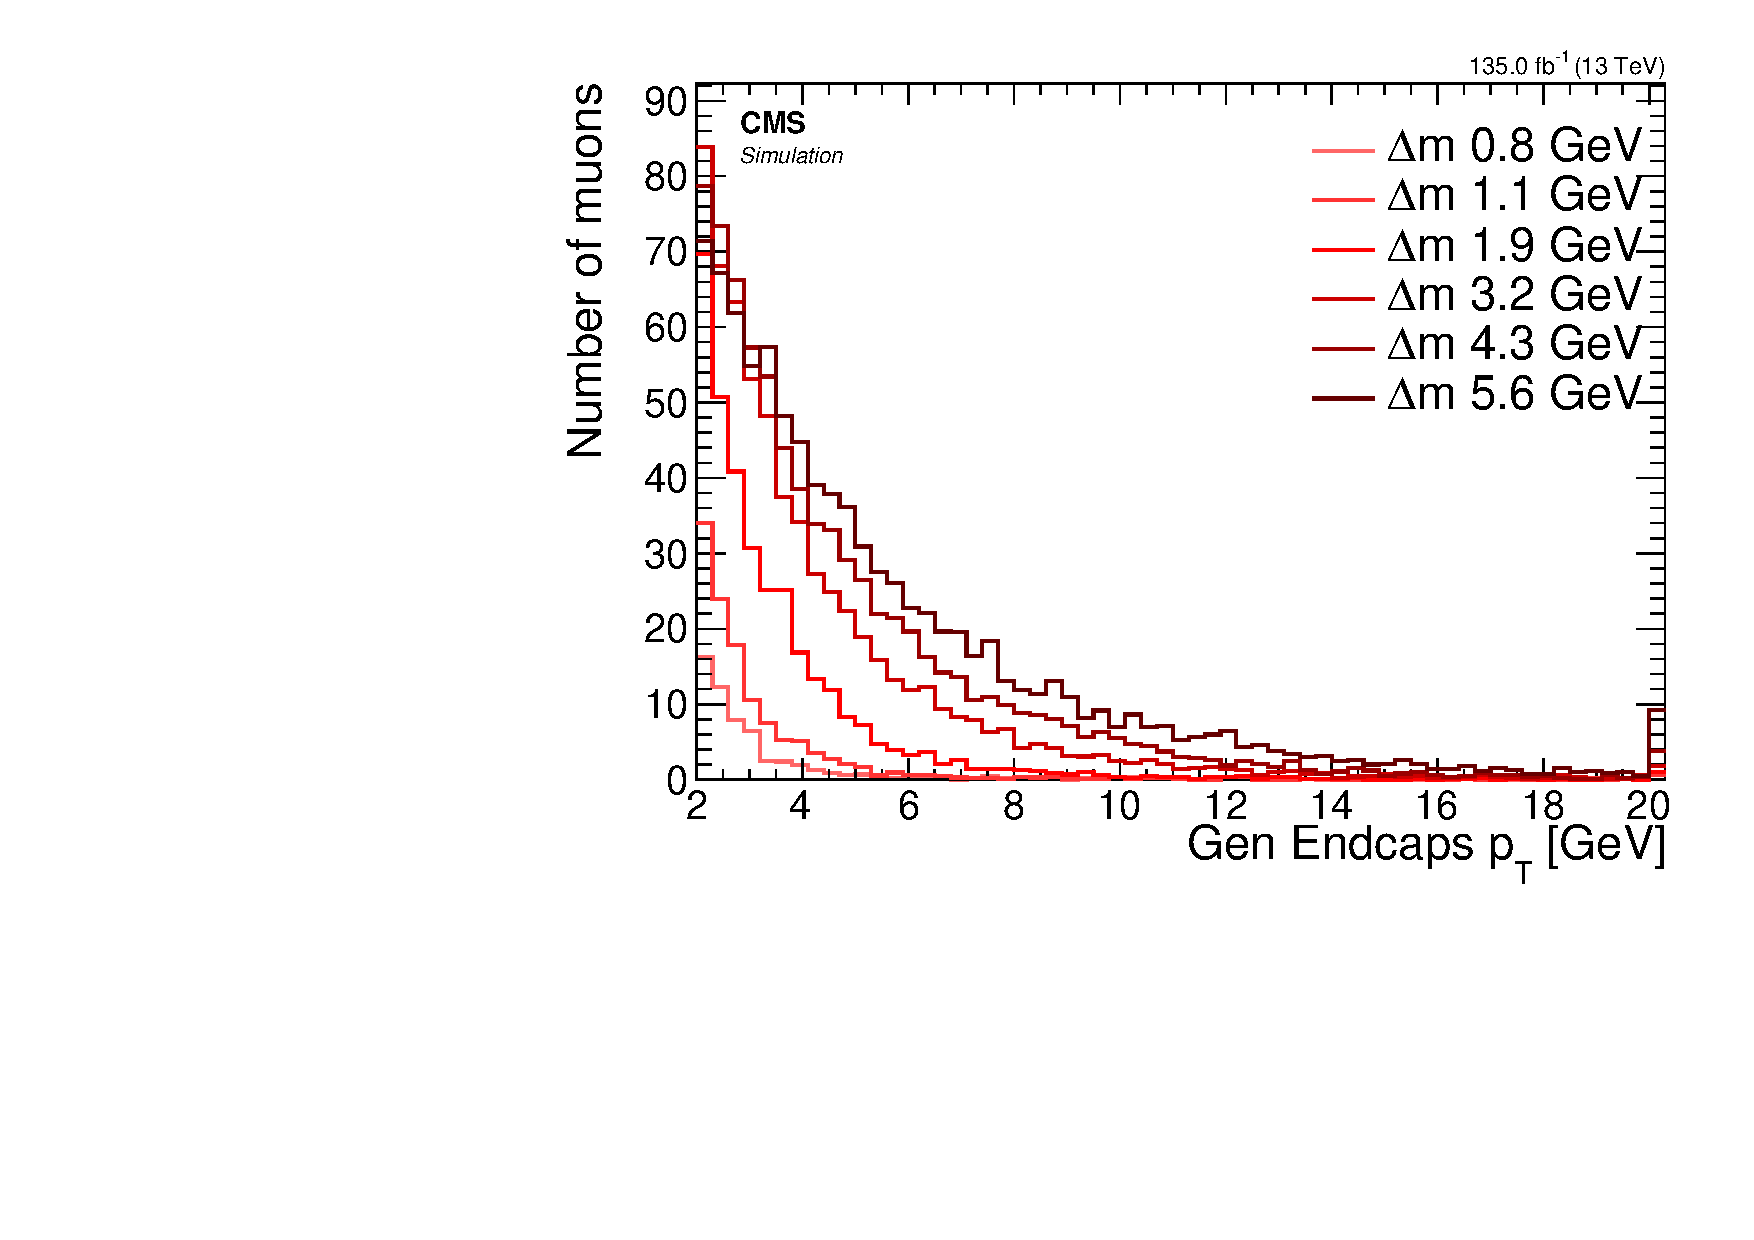
\includegraphics[width=0.48\linewidth]{plots/signal_muons_gen/none_Muons_pt_endcape.pdf}  \\
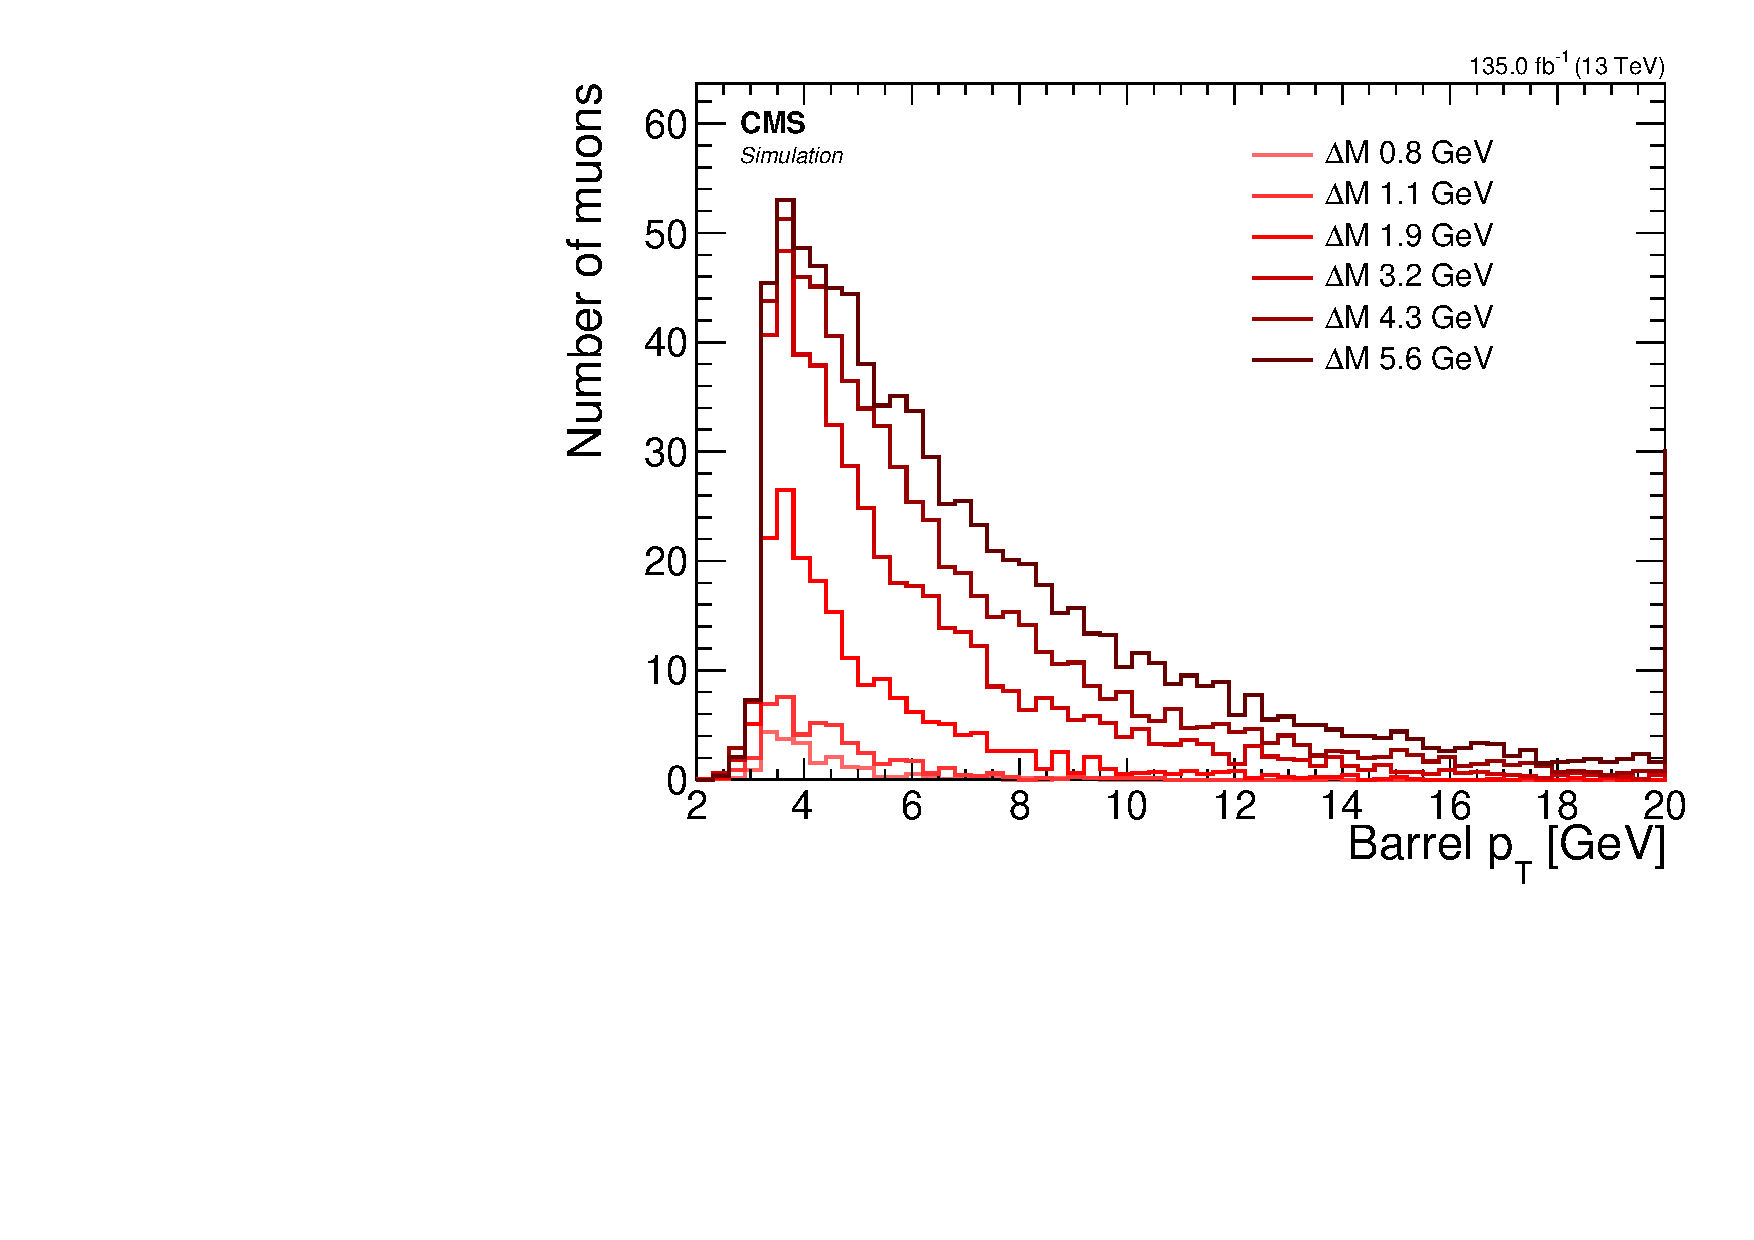
\includegraphics[width=0.48\linewidth]{plots/signal_muons/none_Muons_pt_barrel.pdf} \,
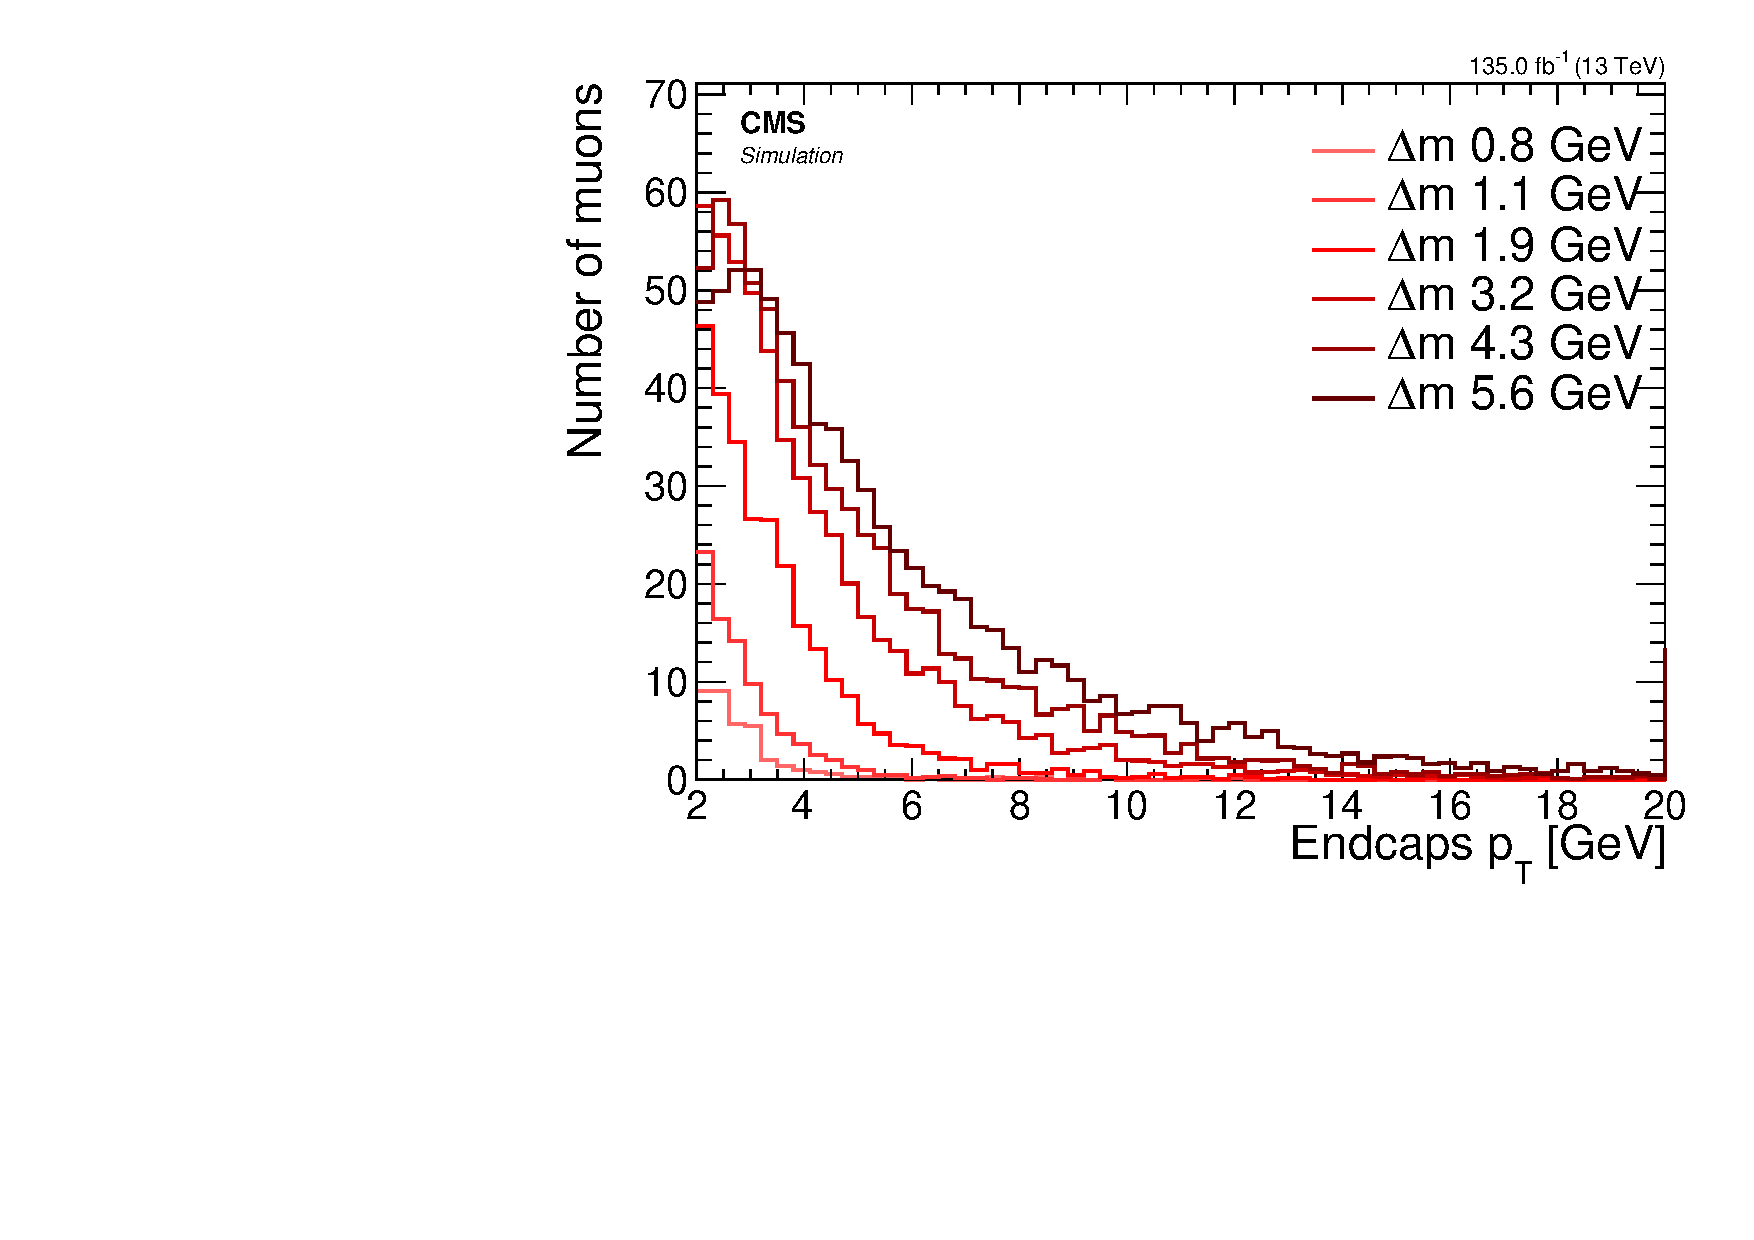
\includegraphics[width=0.48\linewidth]{plots/signal_muons/none_Muons_pt_endcape.pdf}  \\
\caption[Signal \pt distributions split into barrel and endcaps]{ Signal inclusive \pt distributions for barrel $\abs{\eta} < 1.2$ (left) and endcaps $\abs{\eta} \geq 1.2$ (right) at generator level (top) and reconstruction level passing analysis selection (bottom).}
\label{fig:signal-pt-barrel-endcaps}
\end{figure}

The picture becomes much clearer when the reconstruction efficiency as a function of \pt is examined. When comparing the generator level distribution of the barrel muons on the top left with its reconstructed counterpart on the bottom left, it can be seen that the barrel is almost completely unable to reconstruct muons with $\pt < 3\GeV$, while the endcaps, shown on the left, are able to do so. As demonstrated in the upcoming sections on \gls{mll} and \gls{dr} (see \ref{sec:gen-invariant-mass} and \ref{sec:lepton-dr}), the relationship between these distributions has consequences for the reshaping of kinematic distributions, as well as signal acceptance in general. Access to low \dm signal points is crucially dependent on the low \pt region of $2 \leq \pt \leq 3.5\GeV$, which is mainly achieved with the help of the muon chamber endcaps, as can be seen here.

Since the barrel and endcaps are seperated by different regions of $\eta$, $\abs{\eta} < 1.2$ for barrel and $\abs{\eta} \geq 1.2$ for endcaps, it is worthwhile taking a look at the $\eta$ distributions of the muons as well. Those can be seen at Figure~\ref{fig:signal-muons-eta}.

\begin{figure}[!htb]
\centering
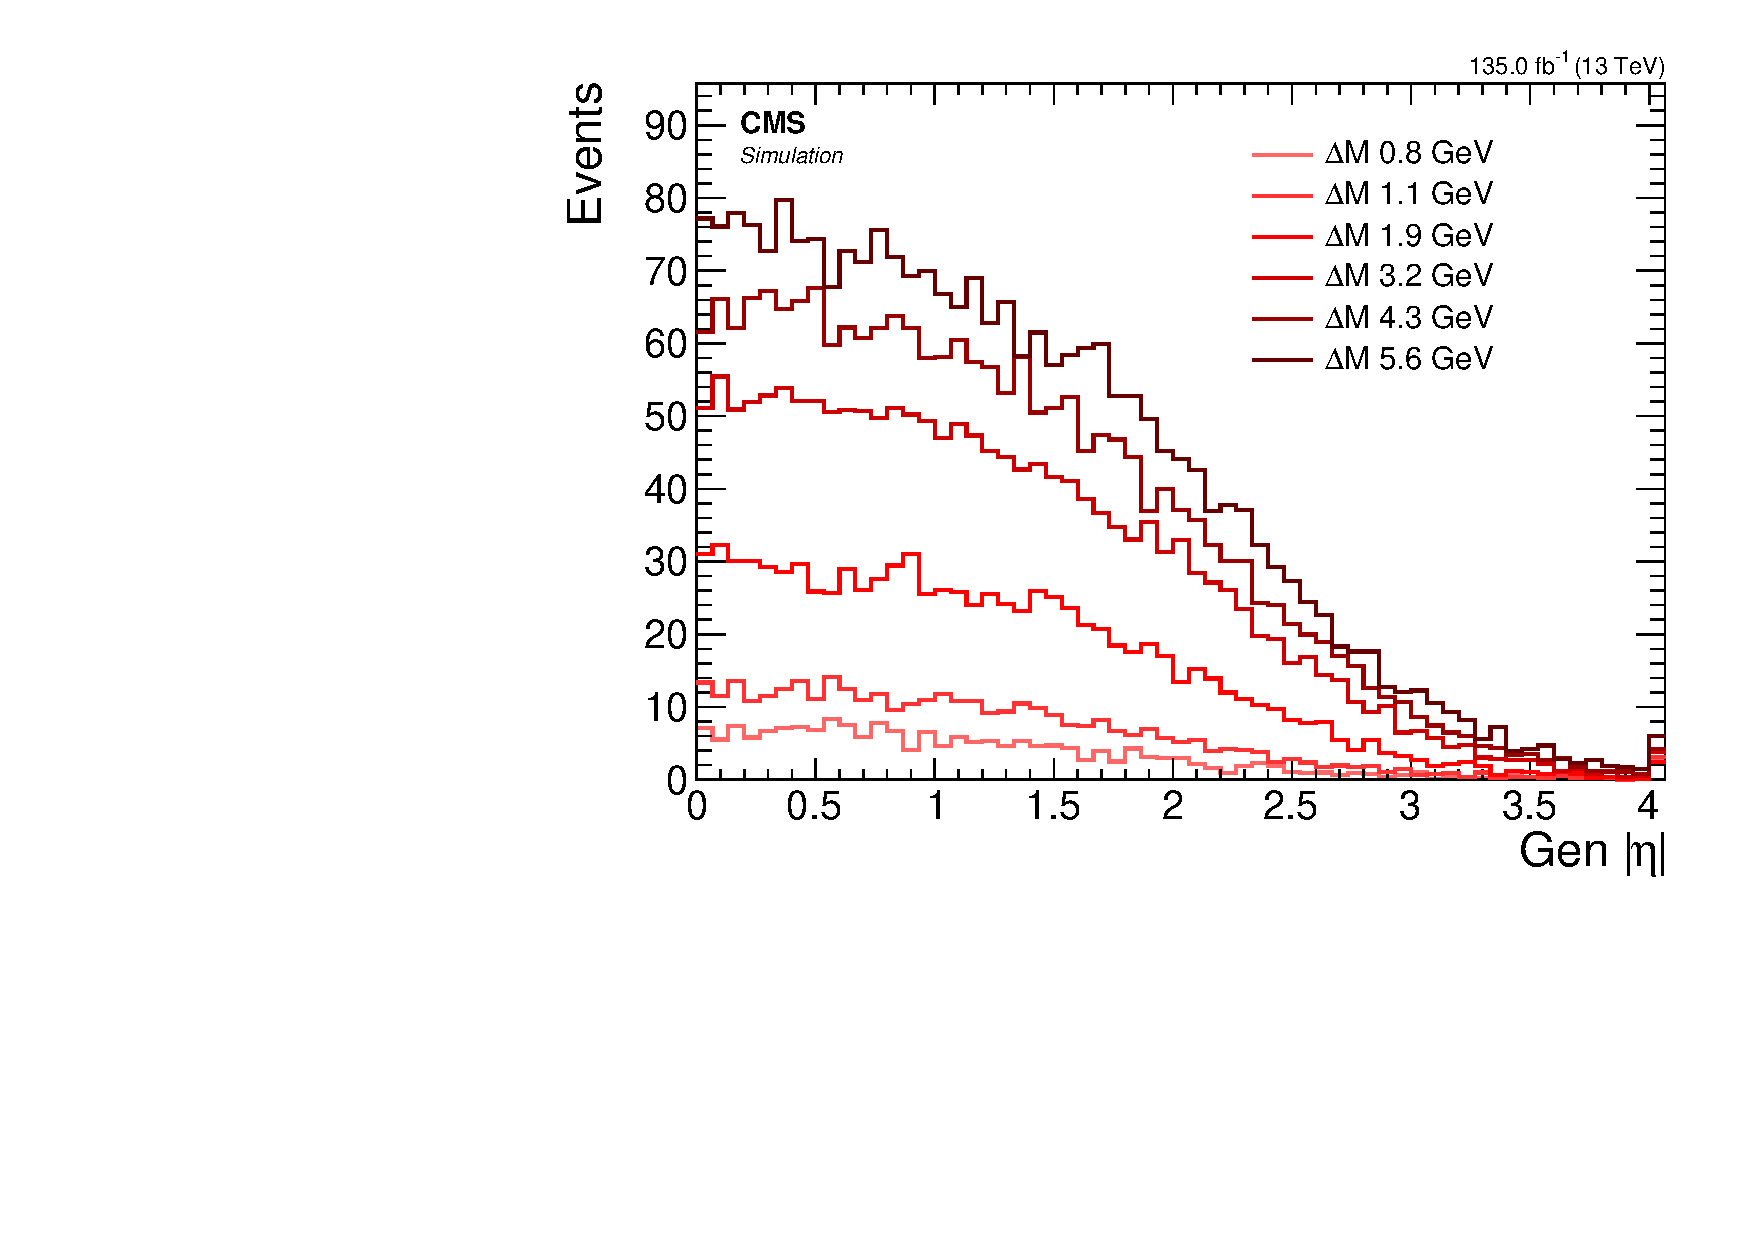
\includegraphics[width=0.32\linewidth]{plots/signal_muons_gen/none_Muons_Eta.pdf} \,
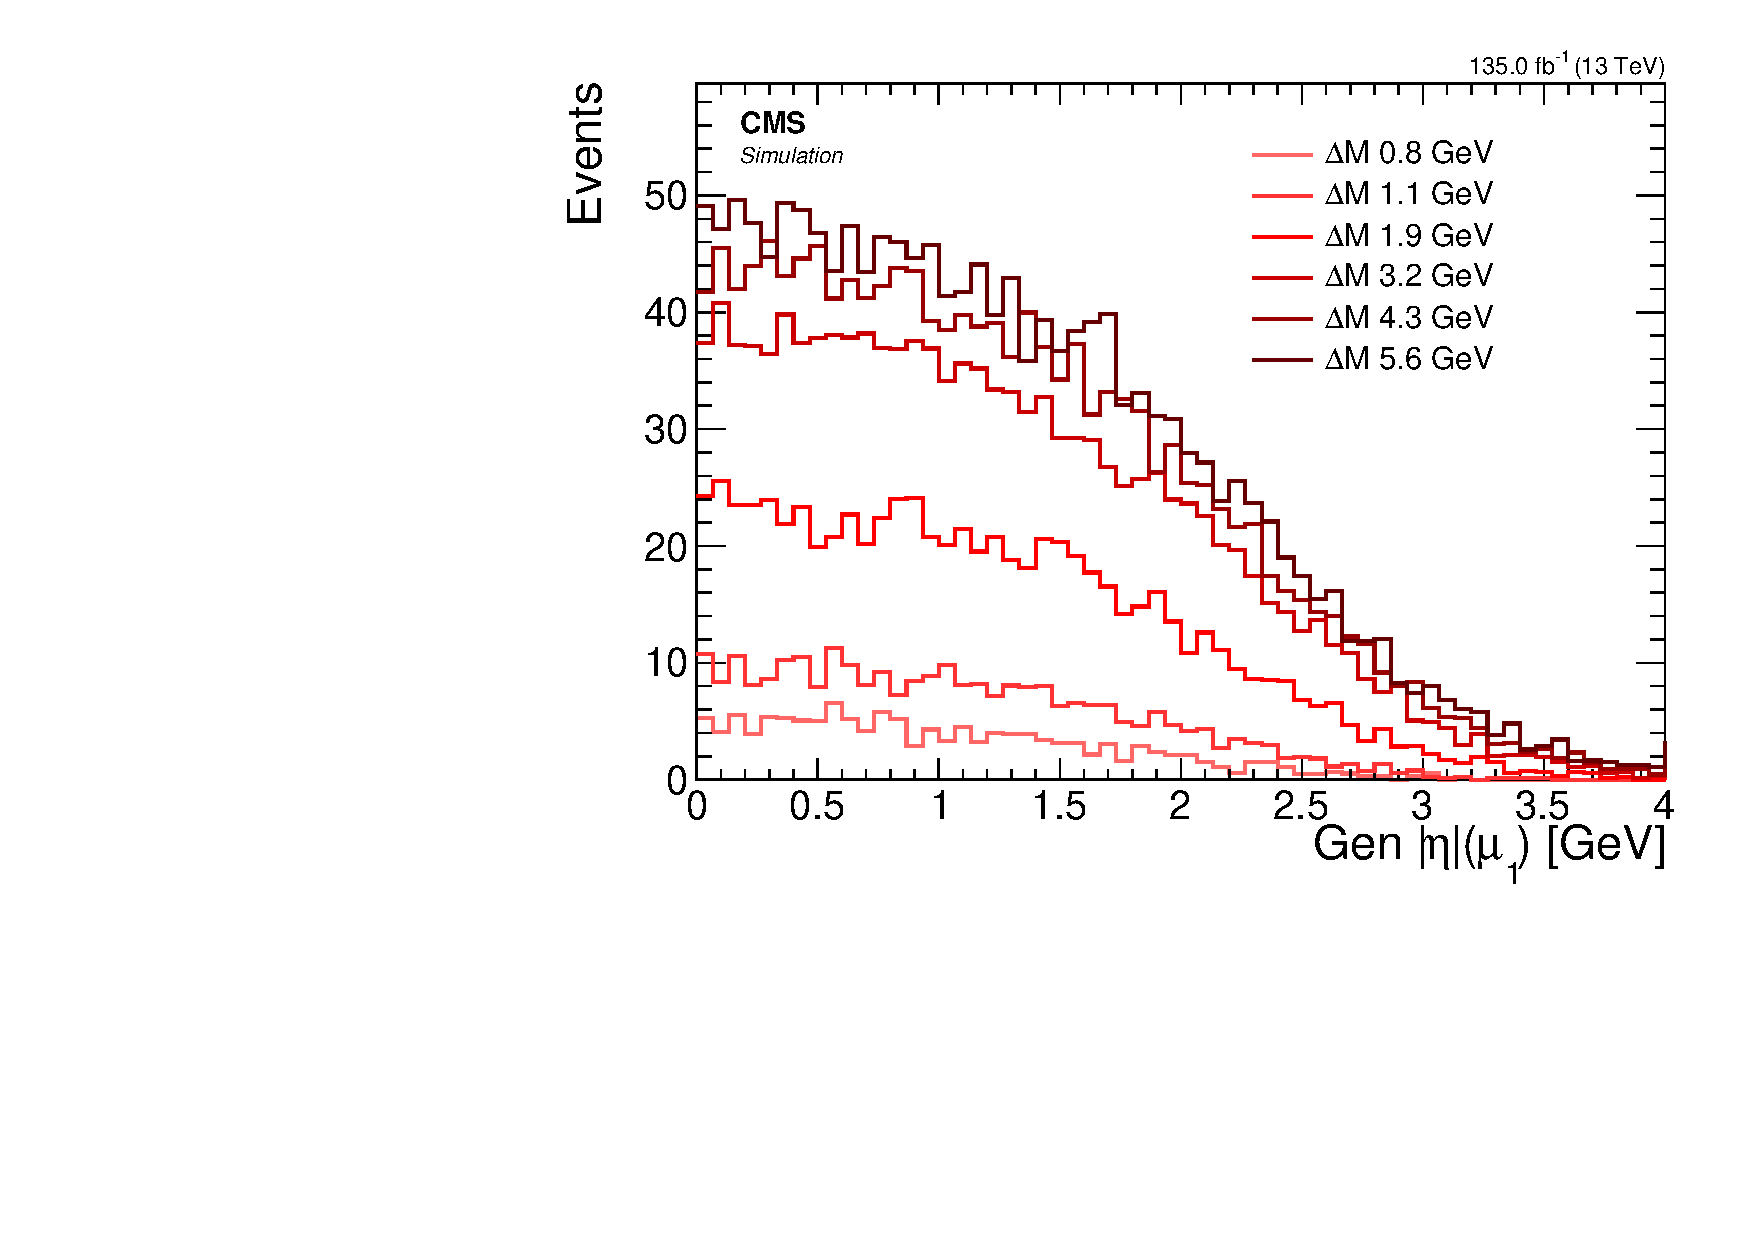
\includegraphics[width=0.32\linewidth]{plots/signal_muons_gen/none_Muons_m1_eta.pdf}  \,
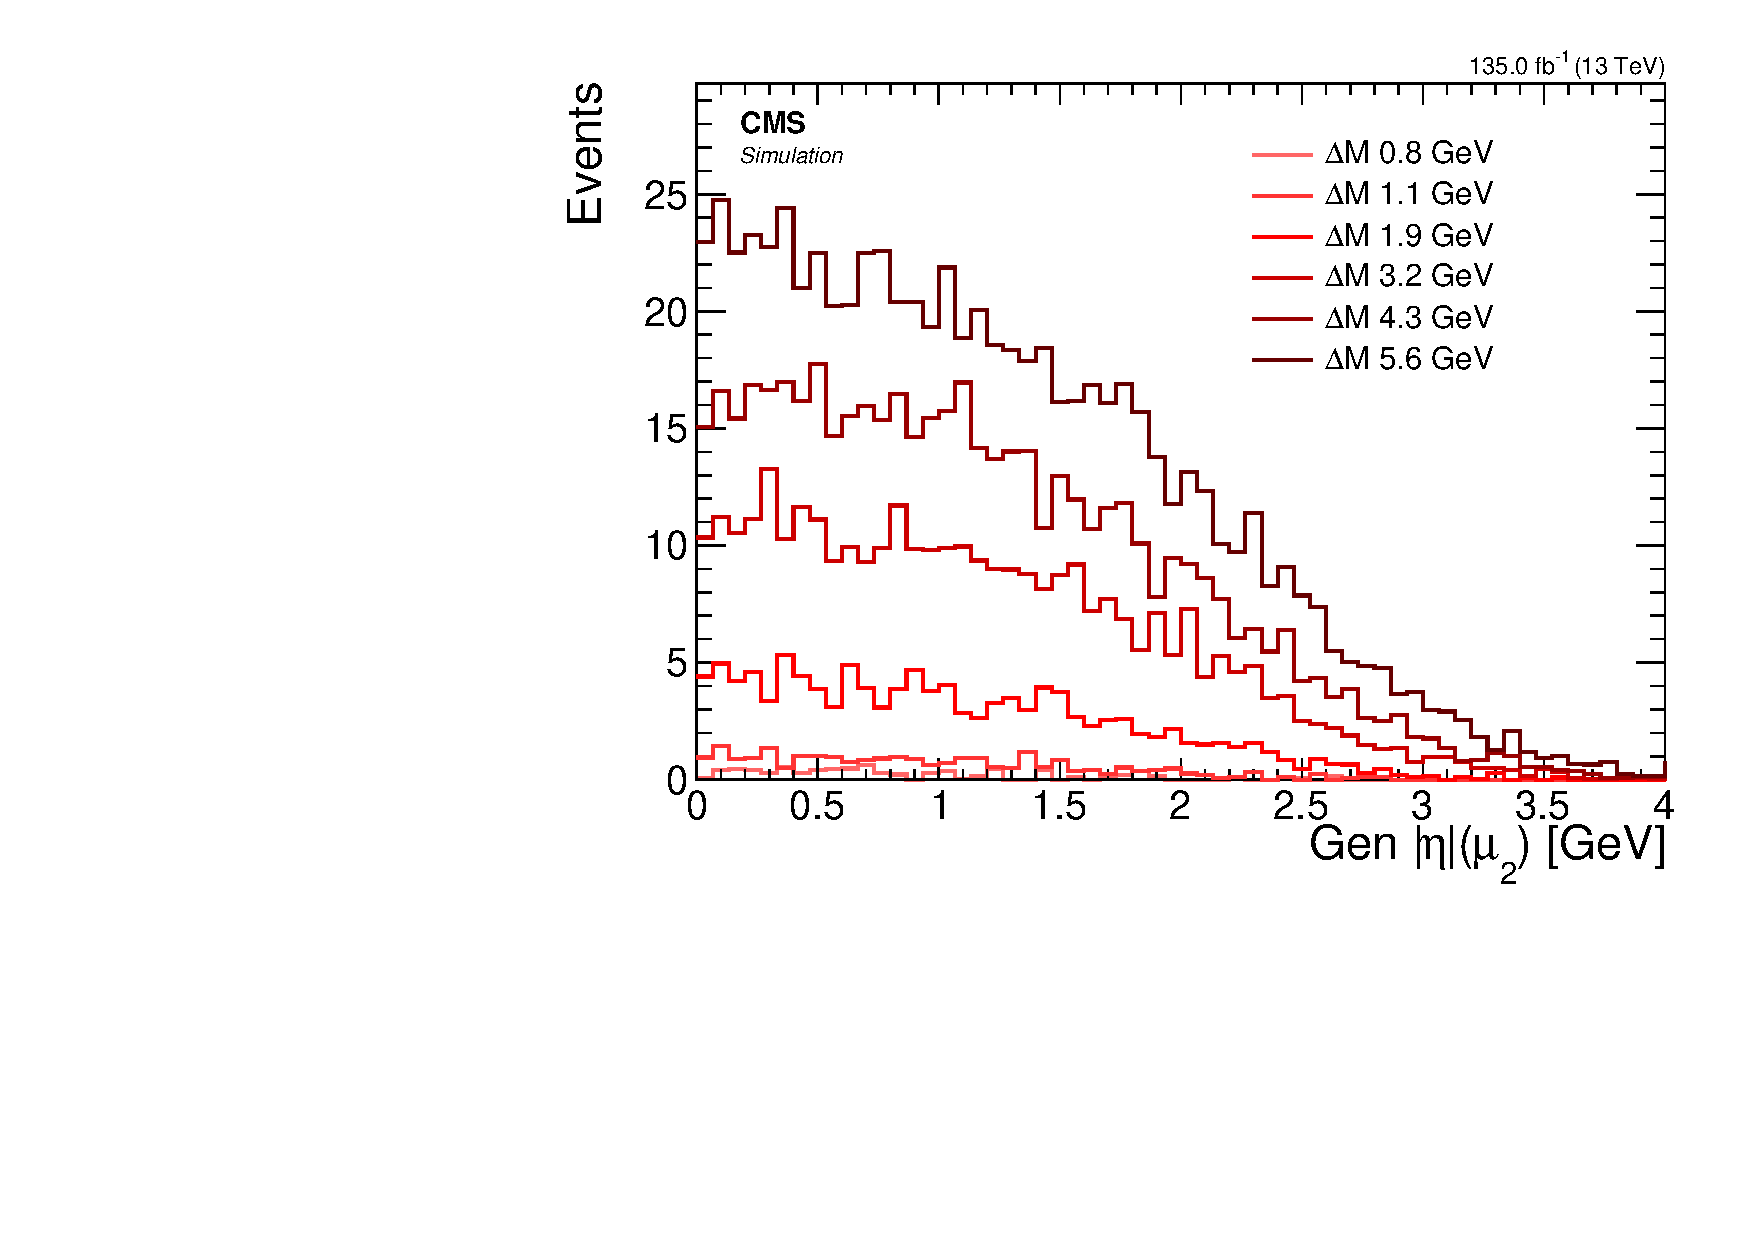
\includegraphics[width=0.32\linewidth]{plots/signal_muons_gen/none_Muons_m2_eta.pdf} \\
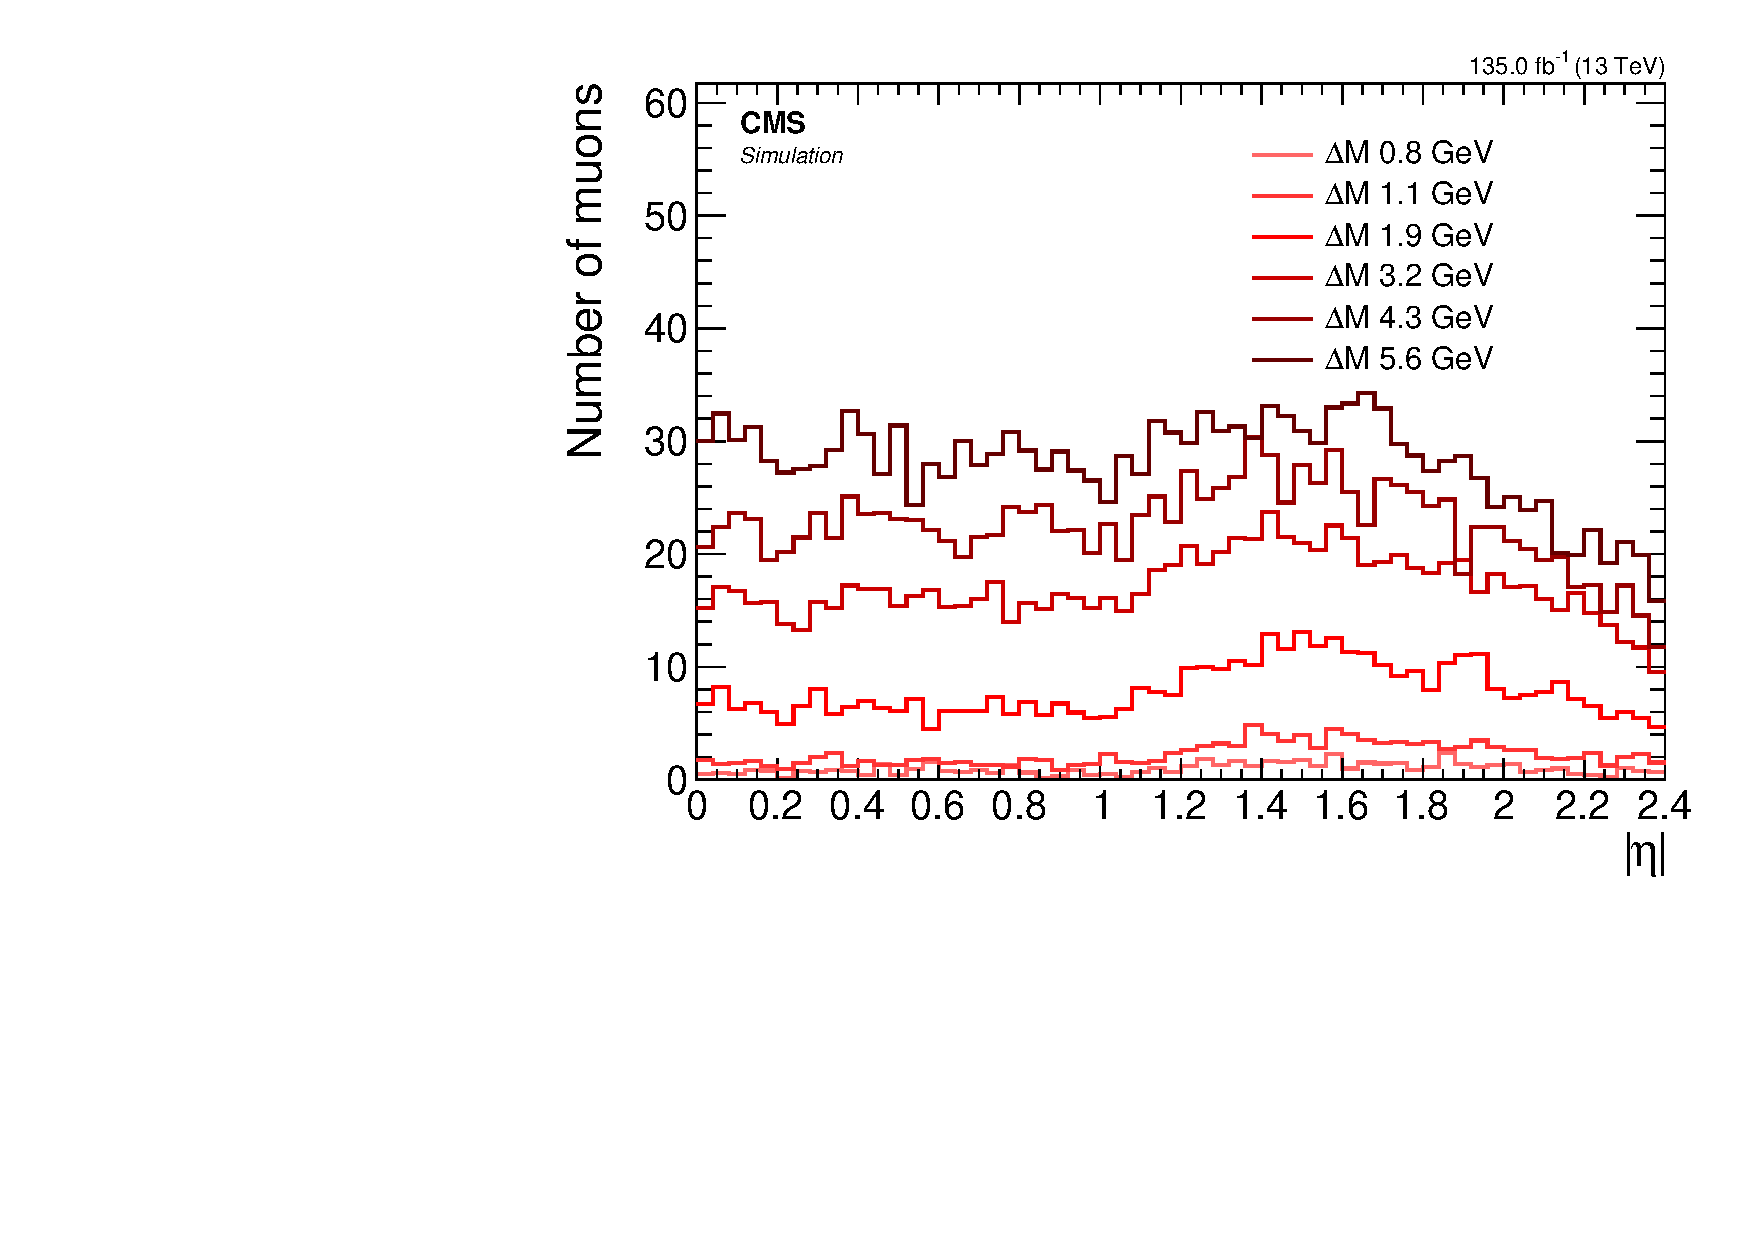
\includegraphics[width=0.32\linewidth]{plots/signal_muons/none_Muons_Eta.pdf} \,
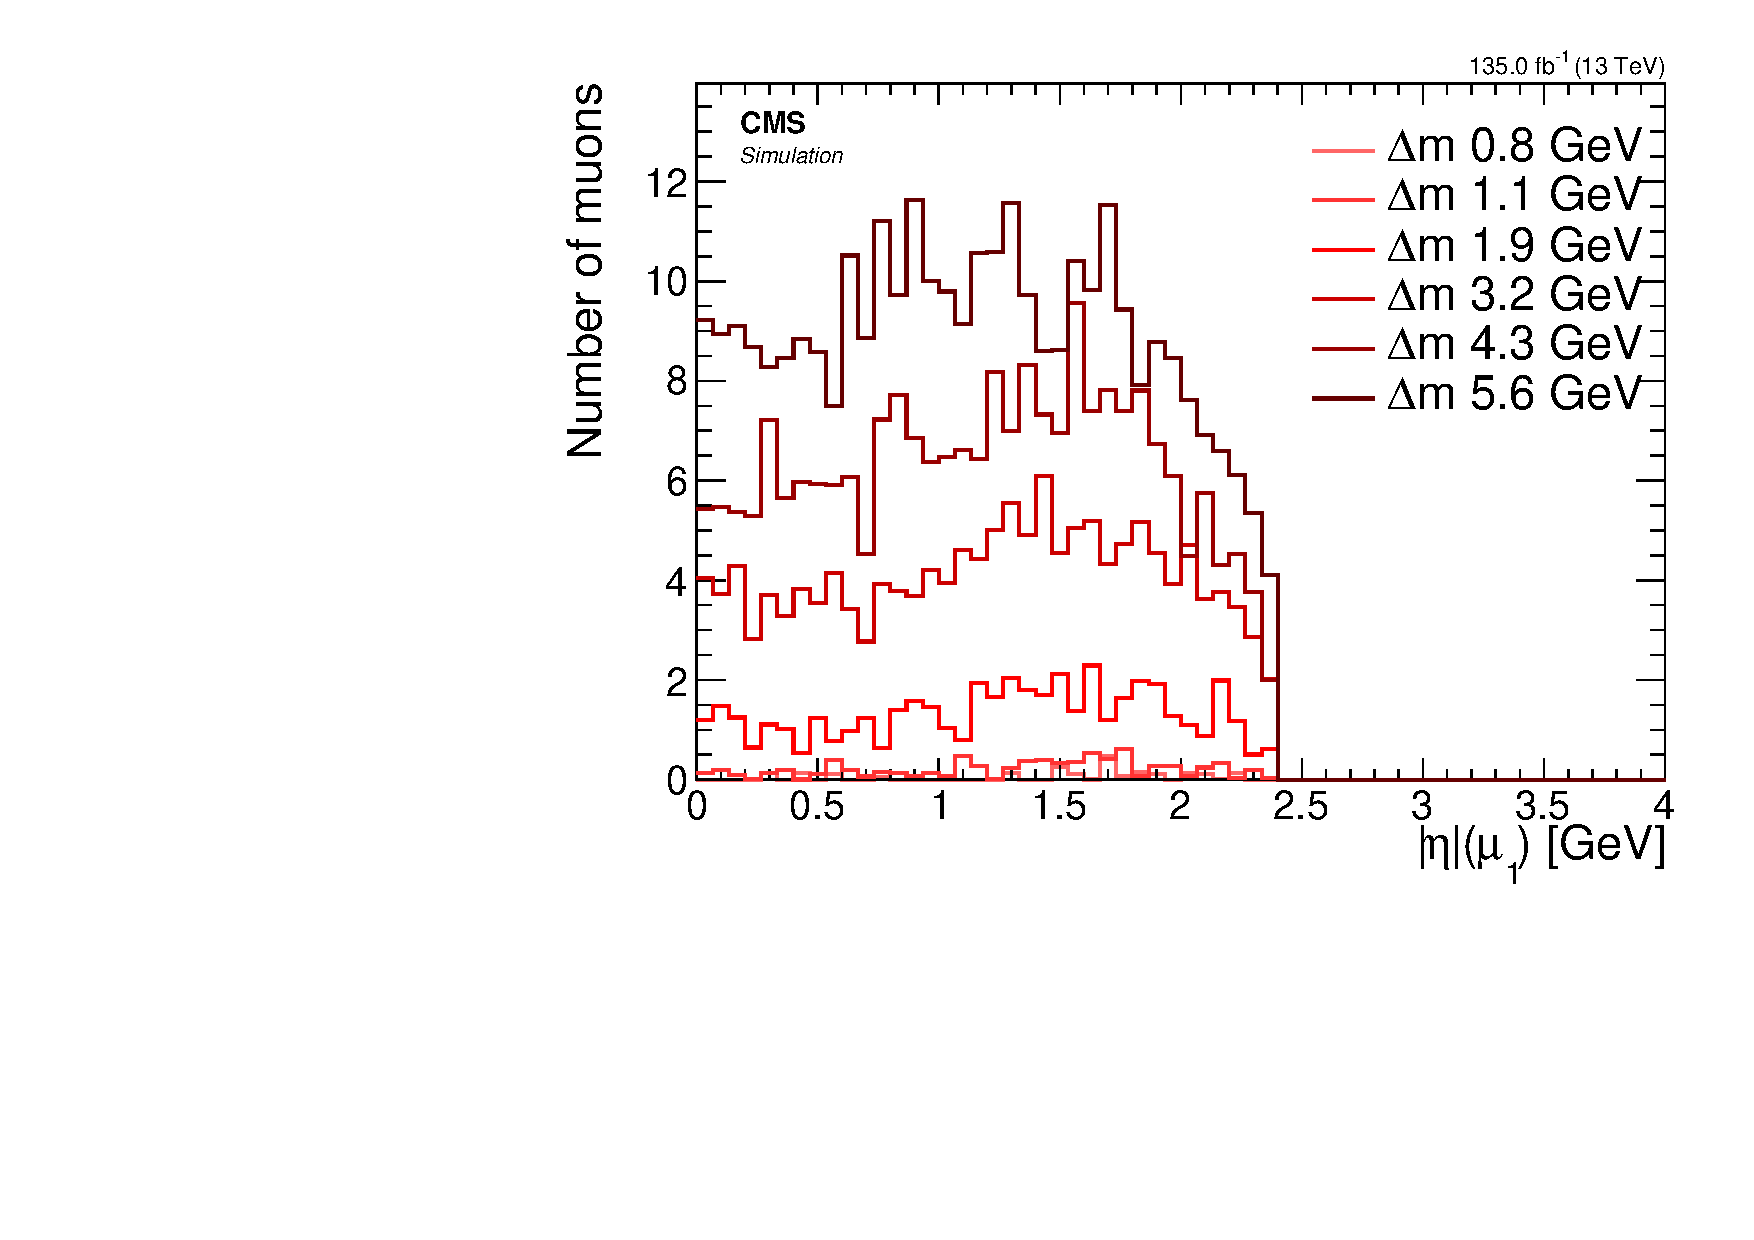
\includegraphics[width=0.32\linewidth]{plots/signal_muons/none_Muons_m1_eta.pdf}  \,
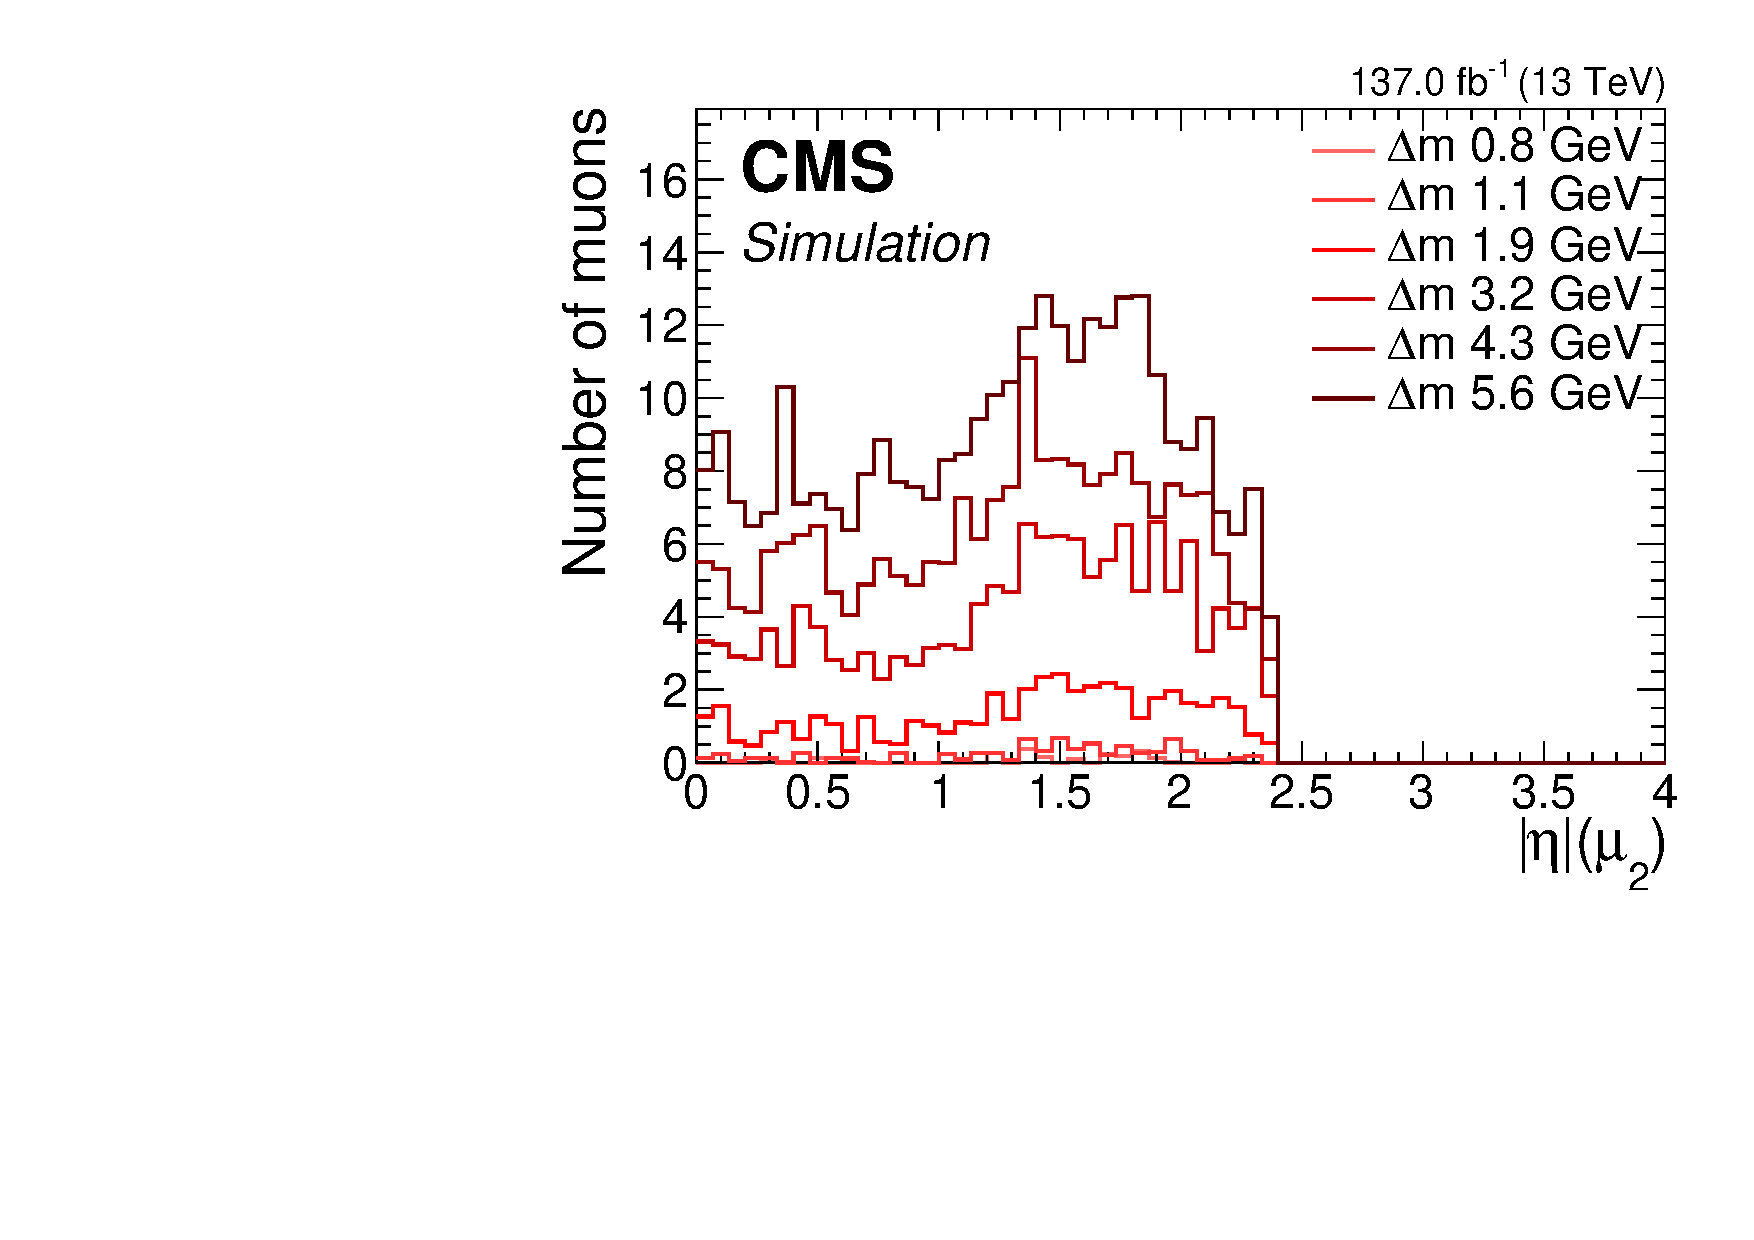
\includegraphics[width=0.32\linewidth]{plots/signal_muons/none_Muons_m2_eta.pdf} \\
\caption[Signal $\abs{\eta}$ distributions]{ Signal $\abs{\eta}$ distributions for inclusive (left), leading muon $\mu_1$ (middle),  subleading muon $\mu_2$ (right) at generator level (top) and reconstruction level passing analysis selection (bottom). }
\label{fig:signal-muons-eta}
\end{figure}

The muons analysis selection only selects muons within the tracker range of $\abs{\eta}<2.4$. This is why the muons with $\abs{\eta}>2.4$ are not present in the reconstruction plots on the bottom. It can be seen that the main effect of going from the inclusive $\abs{\eta}$ at the generator level to the reconstructed counterpart is the flattening of the distribution due to the loss of muons with $\abs{\eta}<1.2$ in the barrel for muons with $\pt<3\GeV$.

With the understanding of the reconstruction effects on the \pt and $\eta$ distributions of the muons, an examination of other kinematic variables of the dilepton system is now possible.

\clearpage

\subsubsection{Invariant mass \gls{mll}}
\label{sec:gen-invariant-mass}

The invariant mass of the two leptons resulting from the decay of the \neutt has a unique shape due to the limited allowed phase space of the leptons as part of the 3-body decay. As the \neutt decays into \neuto and \ellell through a \PZstar, the allowed phase space of the dilepton pair is restricted to the mass difference between \neutt and \neuto, that is, \dm. Therefore, the \gls{mll} distribution is expected to have an edge at \dm. Distributions of the generator level invariant mass can be seen in Figure~\ref{fig:signal-generator-mll}.

\begin{figure}[!htb]
\centering
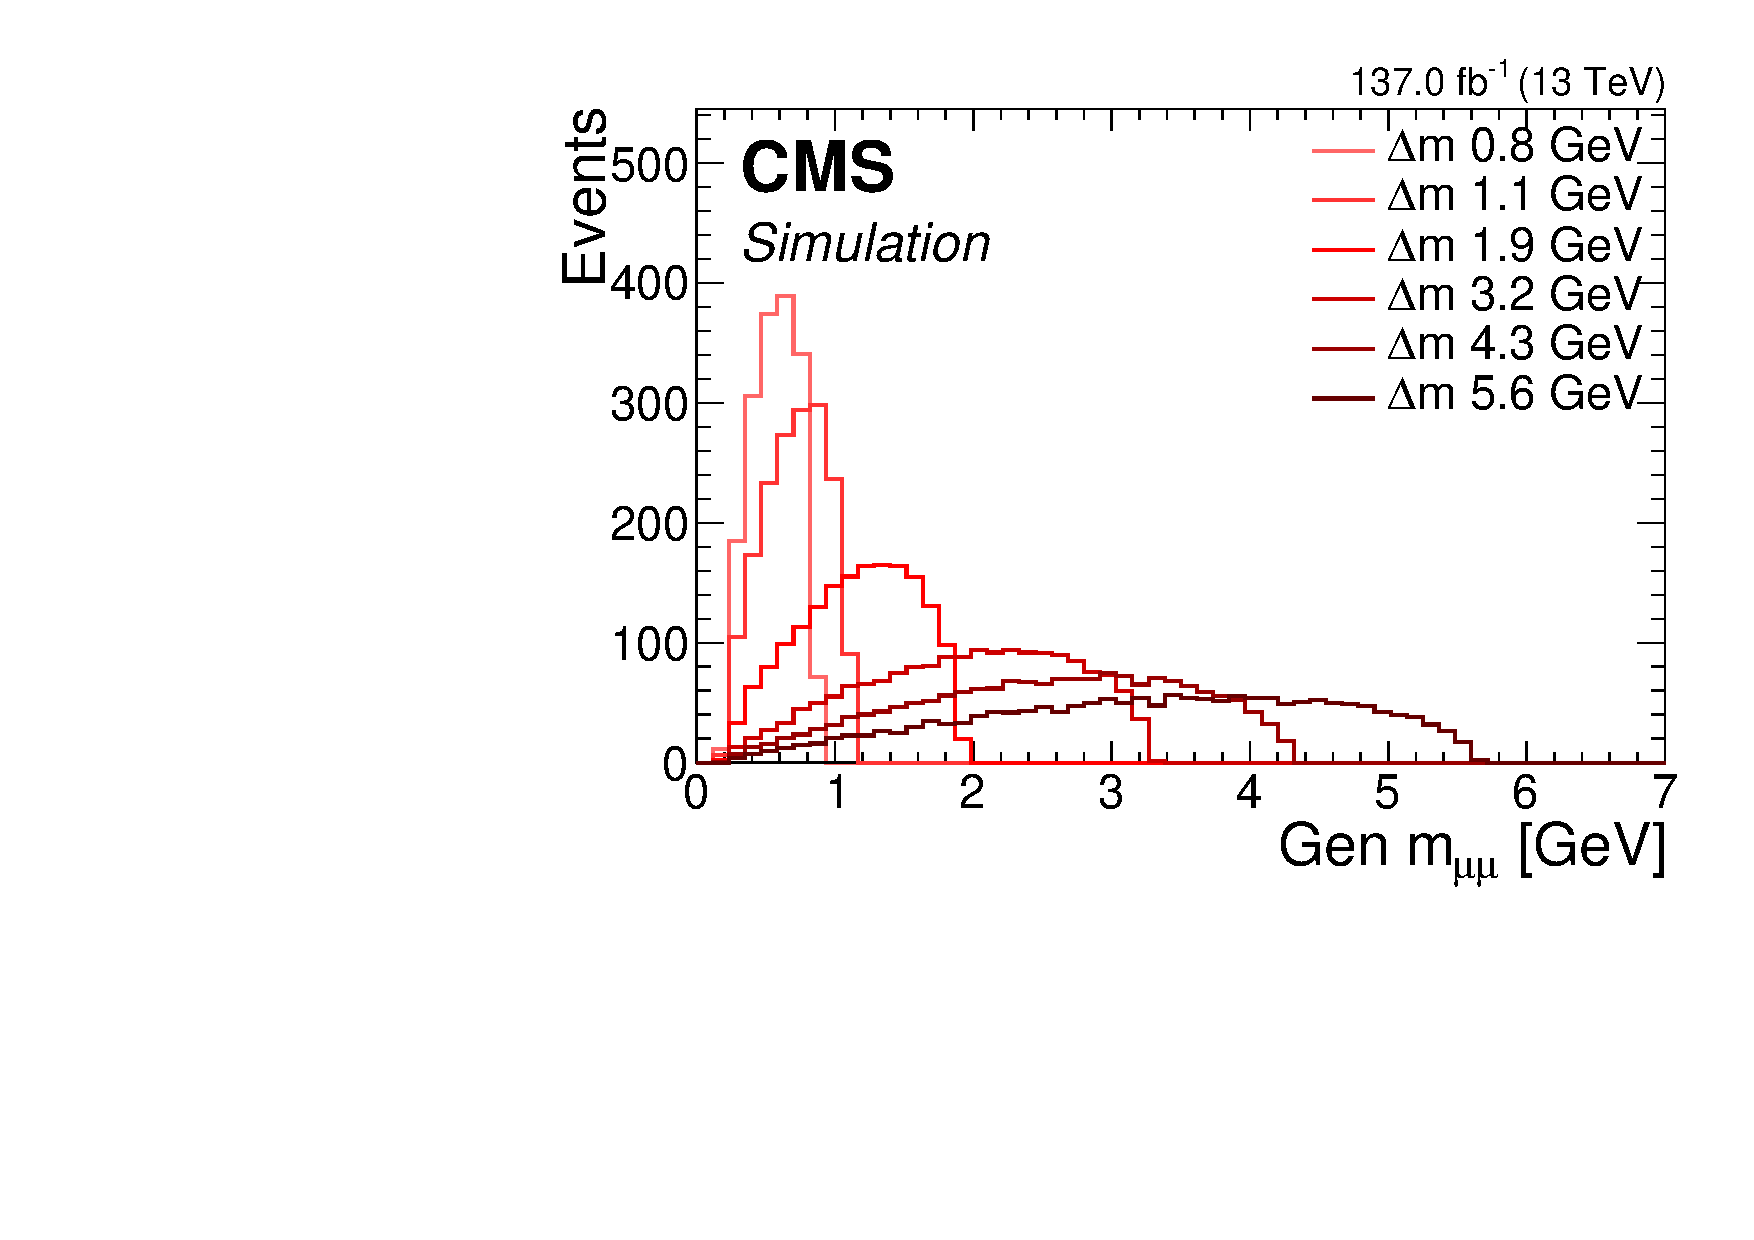
\includegraphics[width=0.32\linewidth]{plots/signal_muons_gen/none_gen_invMass.pdf} \,
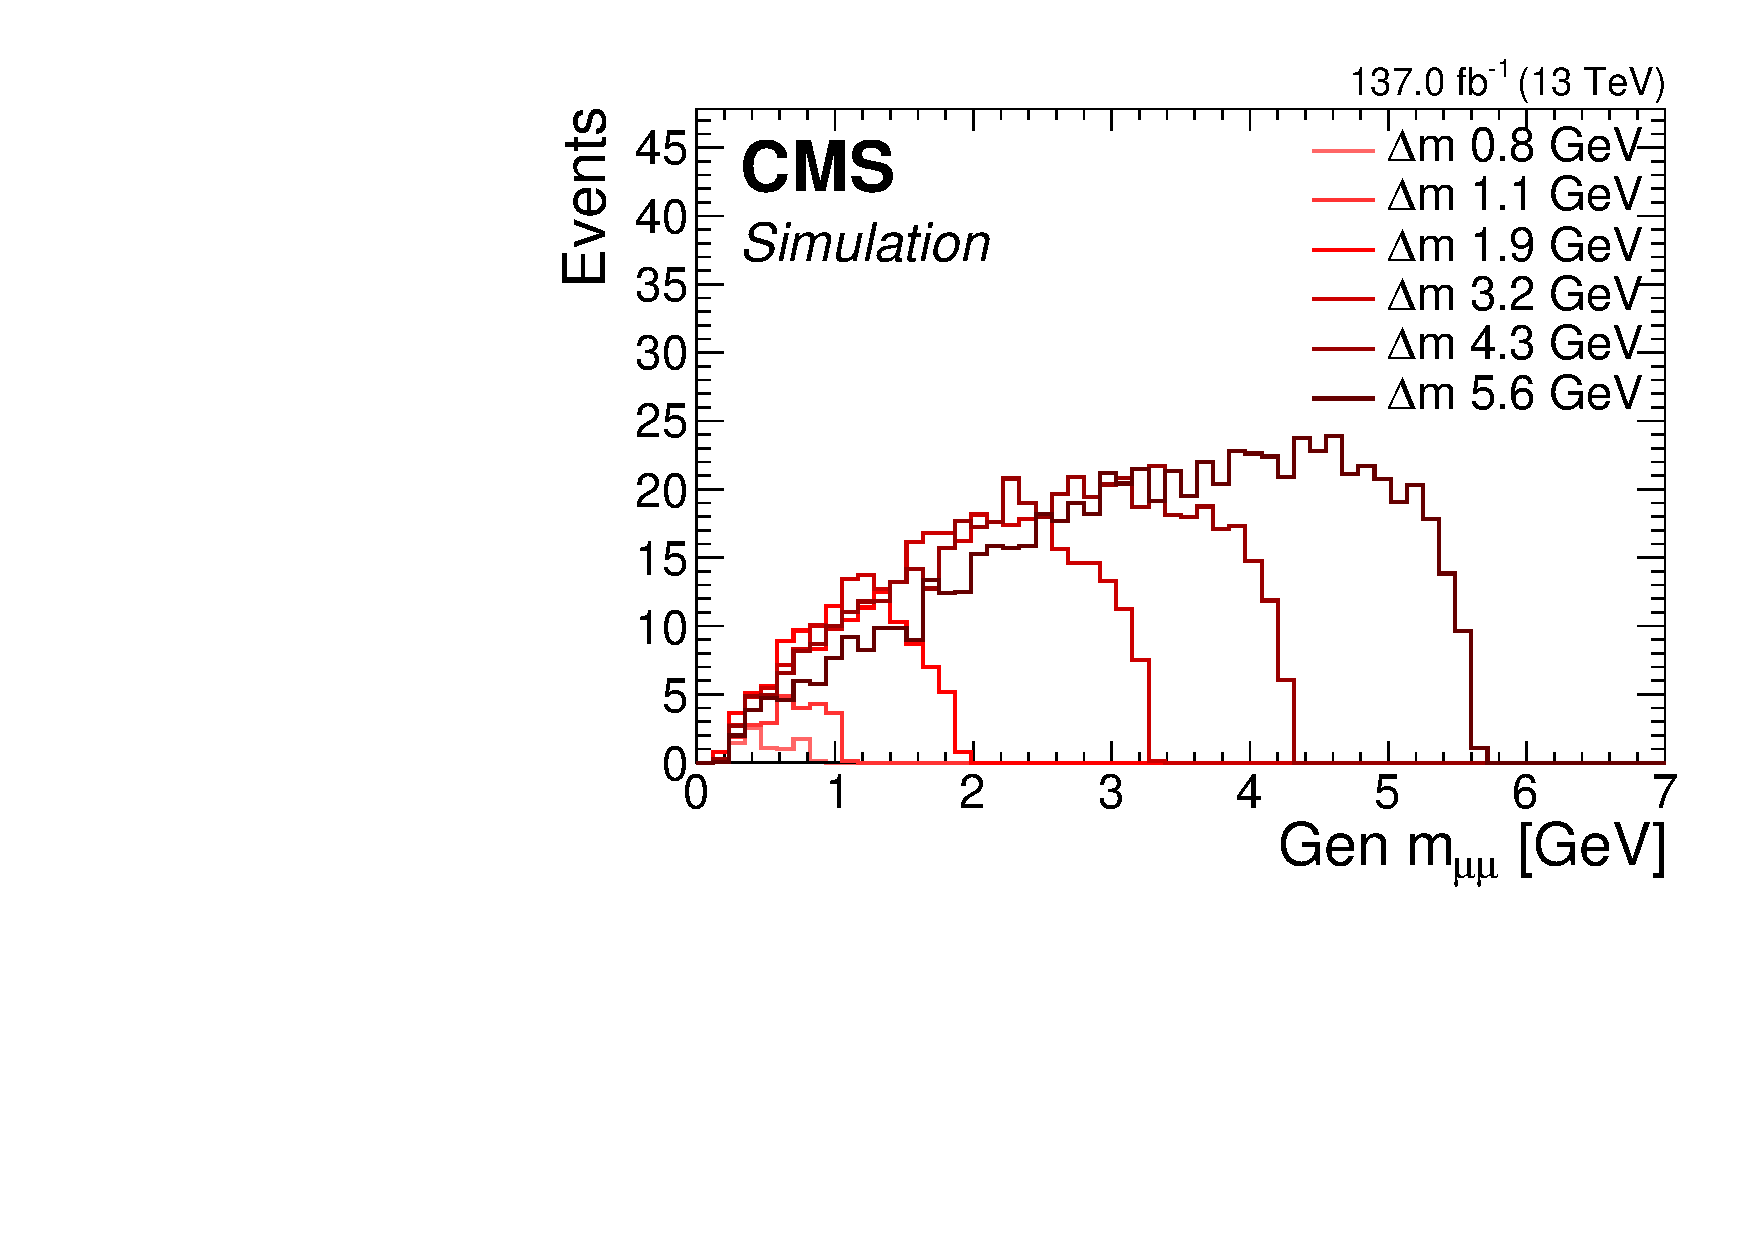
\includegraphics[width=0.32\linewidth]{plots/signal_muons_gen/none_gen_invMass_cut.pdf}  \,
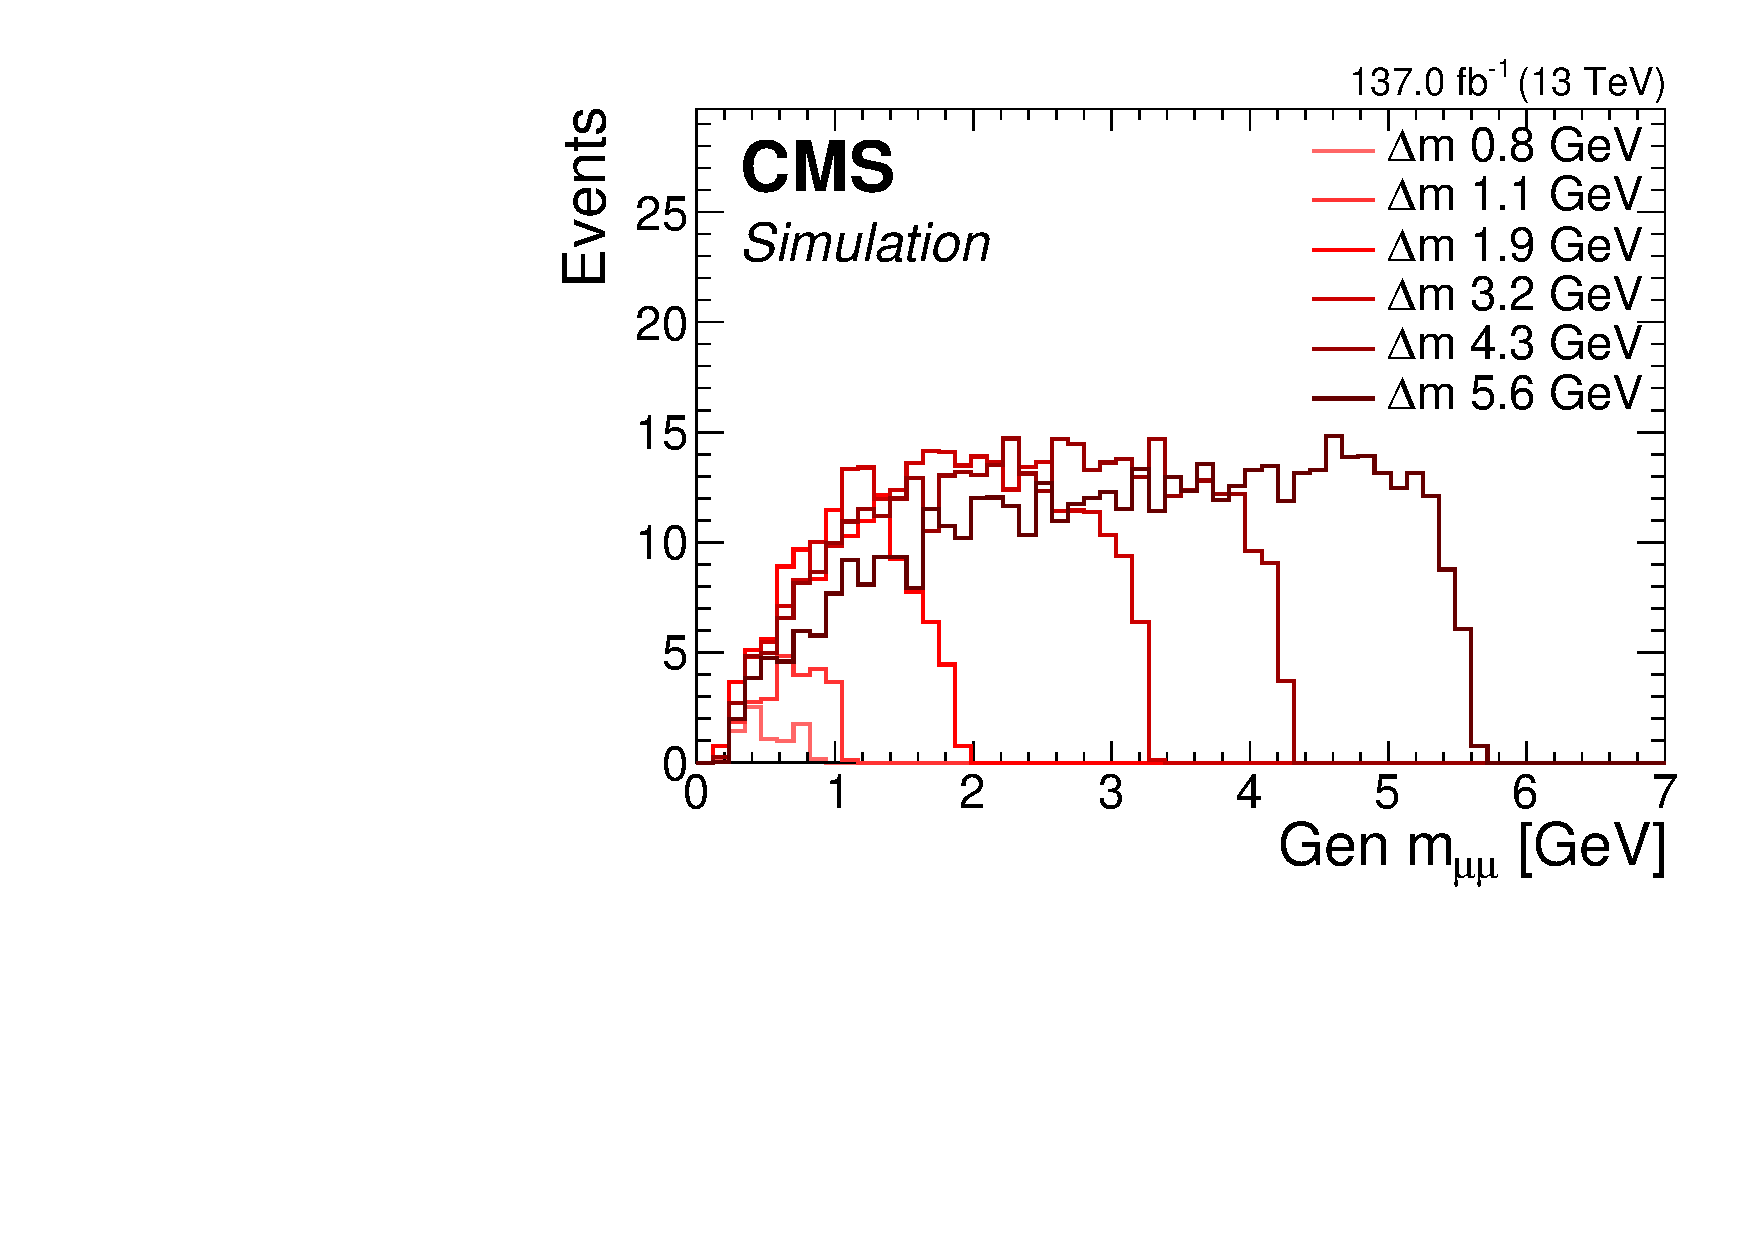
\includegraphics[width=0.32\linewidth]{plots/signal_muons_gen/none_gen_invMass_orth.pdf} \\
\caption[Signal generator level \mll distributions]{ Signal generator level \mll distributions with no cuts (left), with $\pt\left(\mu_i\right)>2\GeV,\,i=1,2$ (middle) and with \gls{sos} orthogonality condition $\pt\left(\mu_i\right)>2\GeV$, $\pt\left(\mu_2\right)\leq~3.5\GeV\text{ or }\Delta R\leq 0.3$ (right).}
\label{fig:signal-generator-mll}
\end{figure}

The inclusive distribution of the invariant mass of the muons \mmumu is shown on the left. The edge of the \mmumu distribution for each signal point is located right at the corresponding \dm. However, when the muons \pt are cut and required to be $\pt\geq 2\GeV$, the shape of the distribution shifts, and the efficiency in the lower \dm range drops significantly, as depicted in the middle plot. Lastly, the effect of orthogonalizing phase space to the \gls{sos} analysis is demonstrated in the rightmost plot. The effect is strongest in high \dm and quite subtle in low \dm.

To comprehend the reshaping that occurs to the \mmumu shape, the relationship between the \pt of the muons (leading muon denoted $\mu_1$ while subleading muon is denoted $\mu_2$) and the invariant mass is examined. One signal with low \dm of $1.13\GeV$ and one with high \dm of $5.63\GeV$ are selected for this analysis. The distributions are shown in Figure~\ref{fig:signal-gen-invamass-pt}.

\begin{figure}[!htb]
\centering
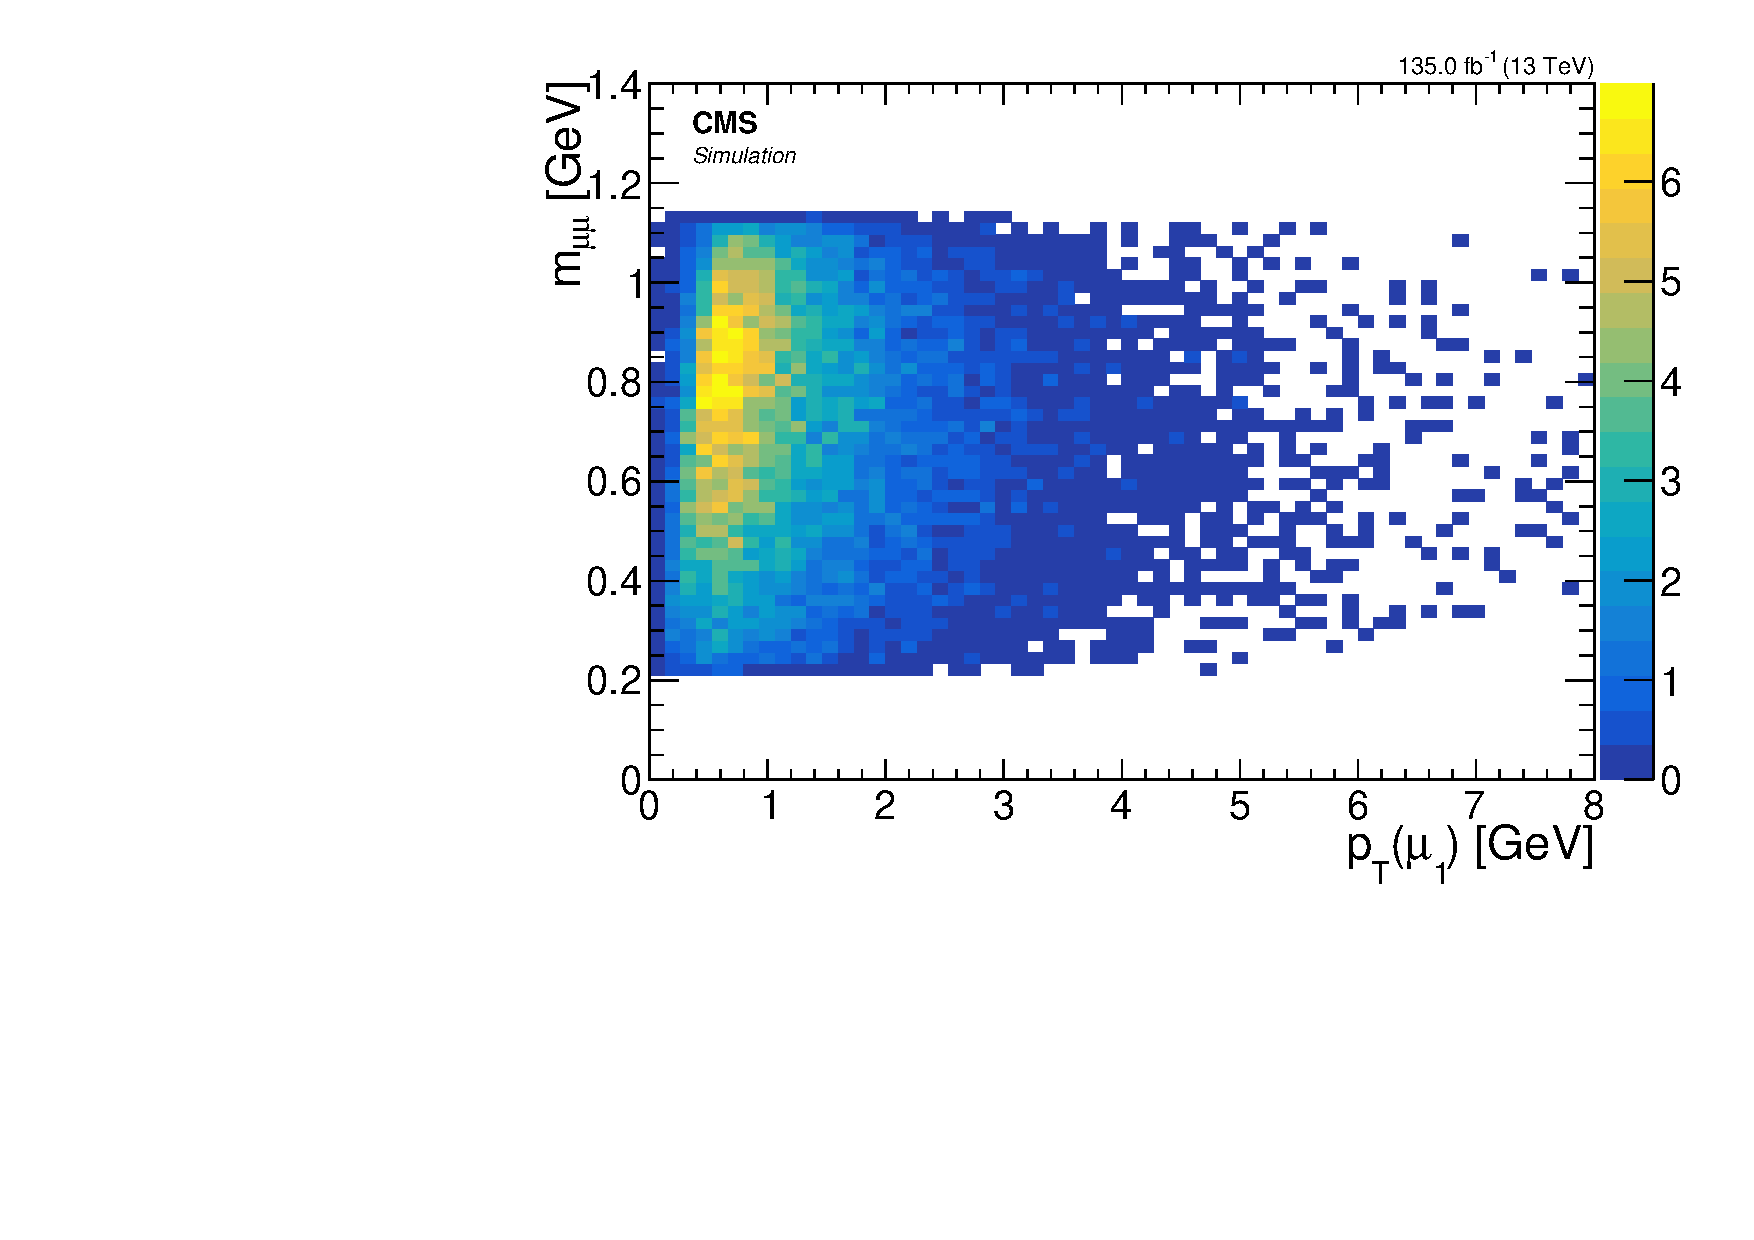
\includegraphics[width=0.48\linewidth]{plots/signal_muons_gen_delta_r_vs_pt/none_gen_invmass_vs_pt_1.pdf} \,
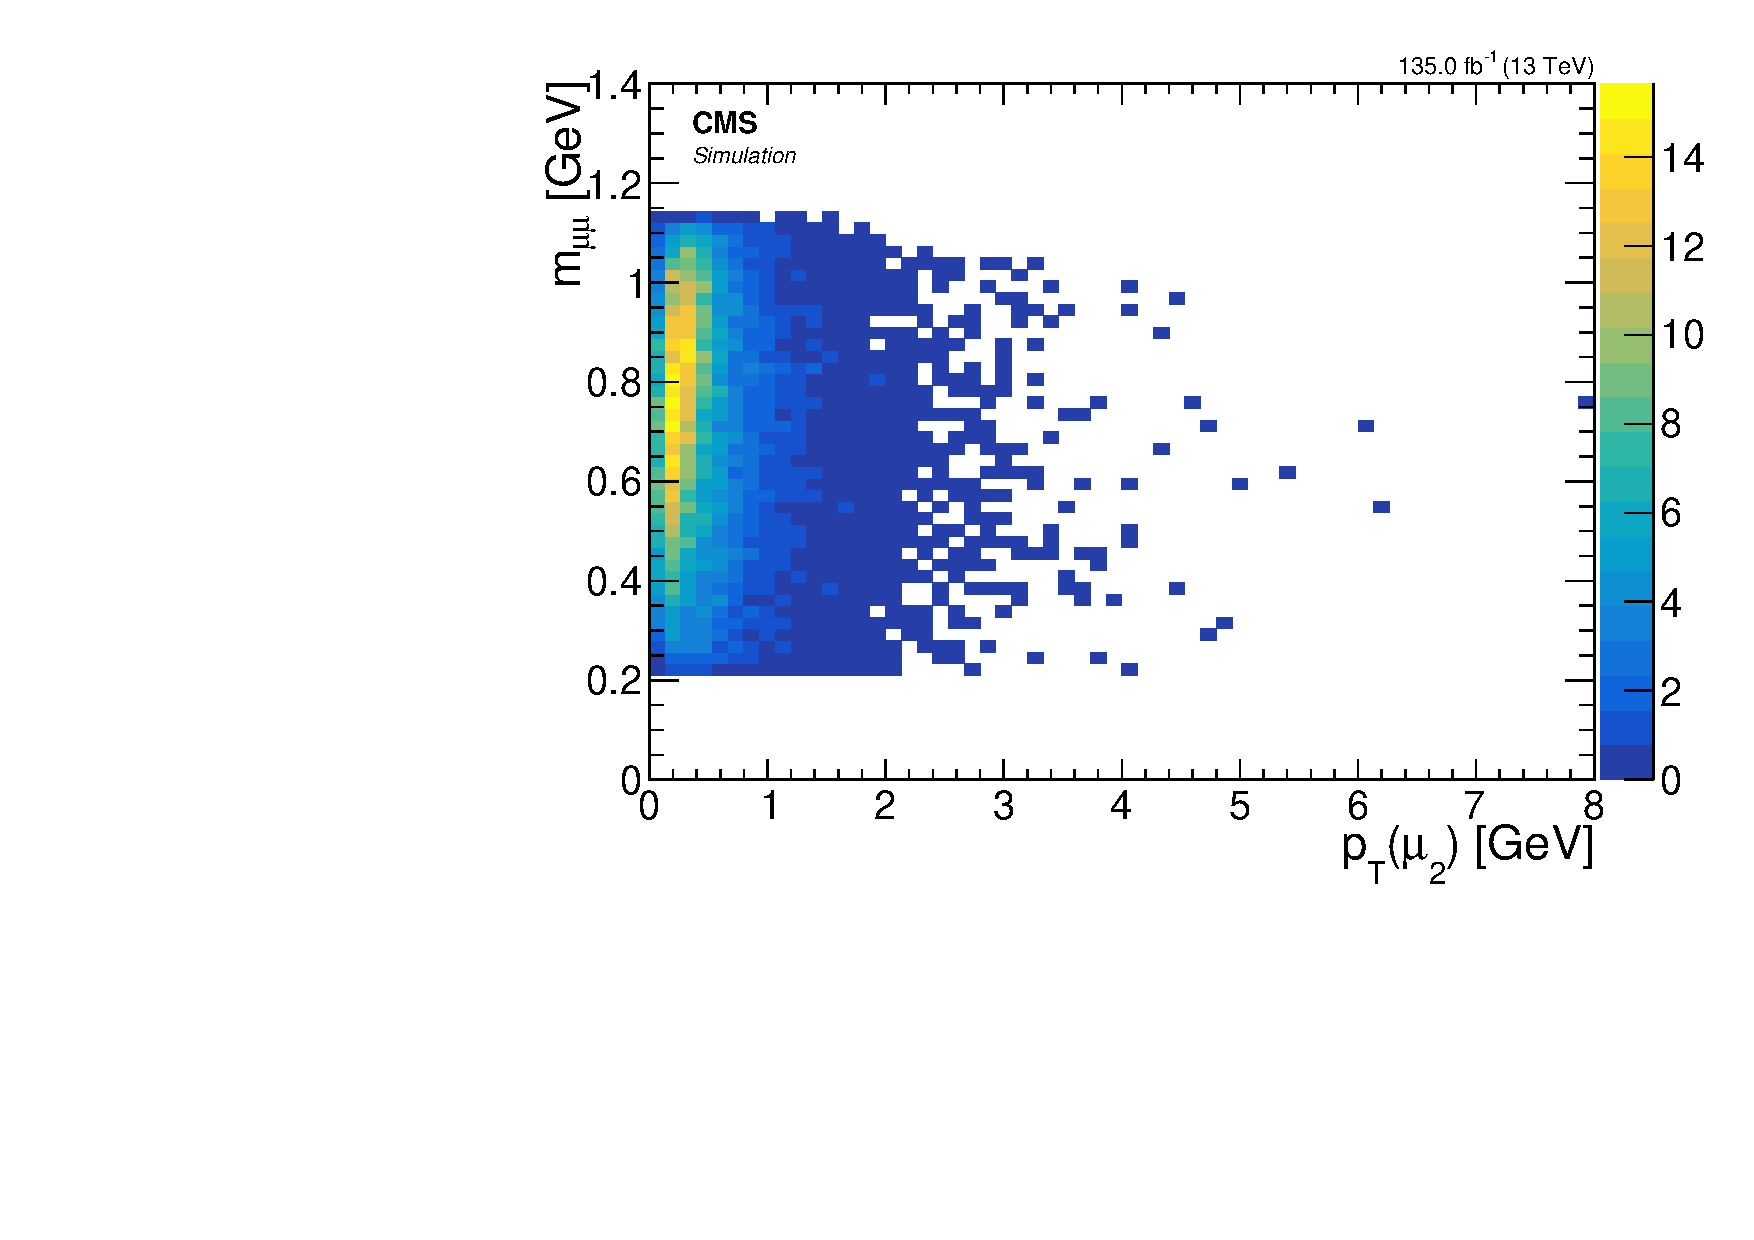
\includegraphics[width=0.48\linewidth]{plots/signal_muons_gen_delta_r_vs_pt/none_gen_invmass_vs_pt_2.pdf}  \\
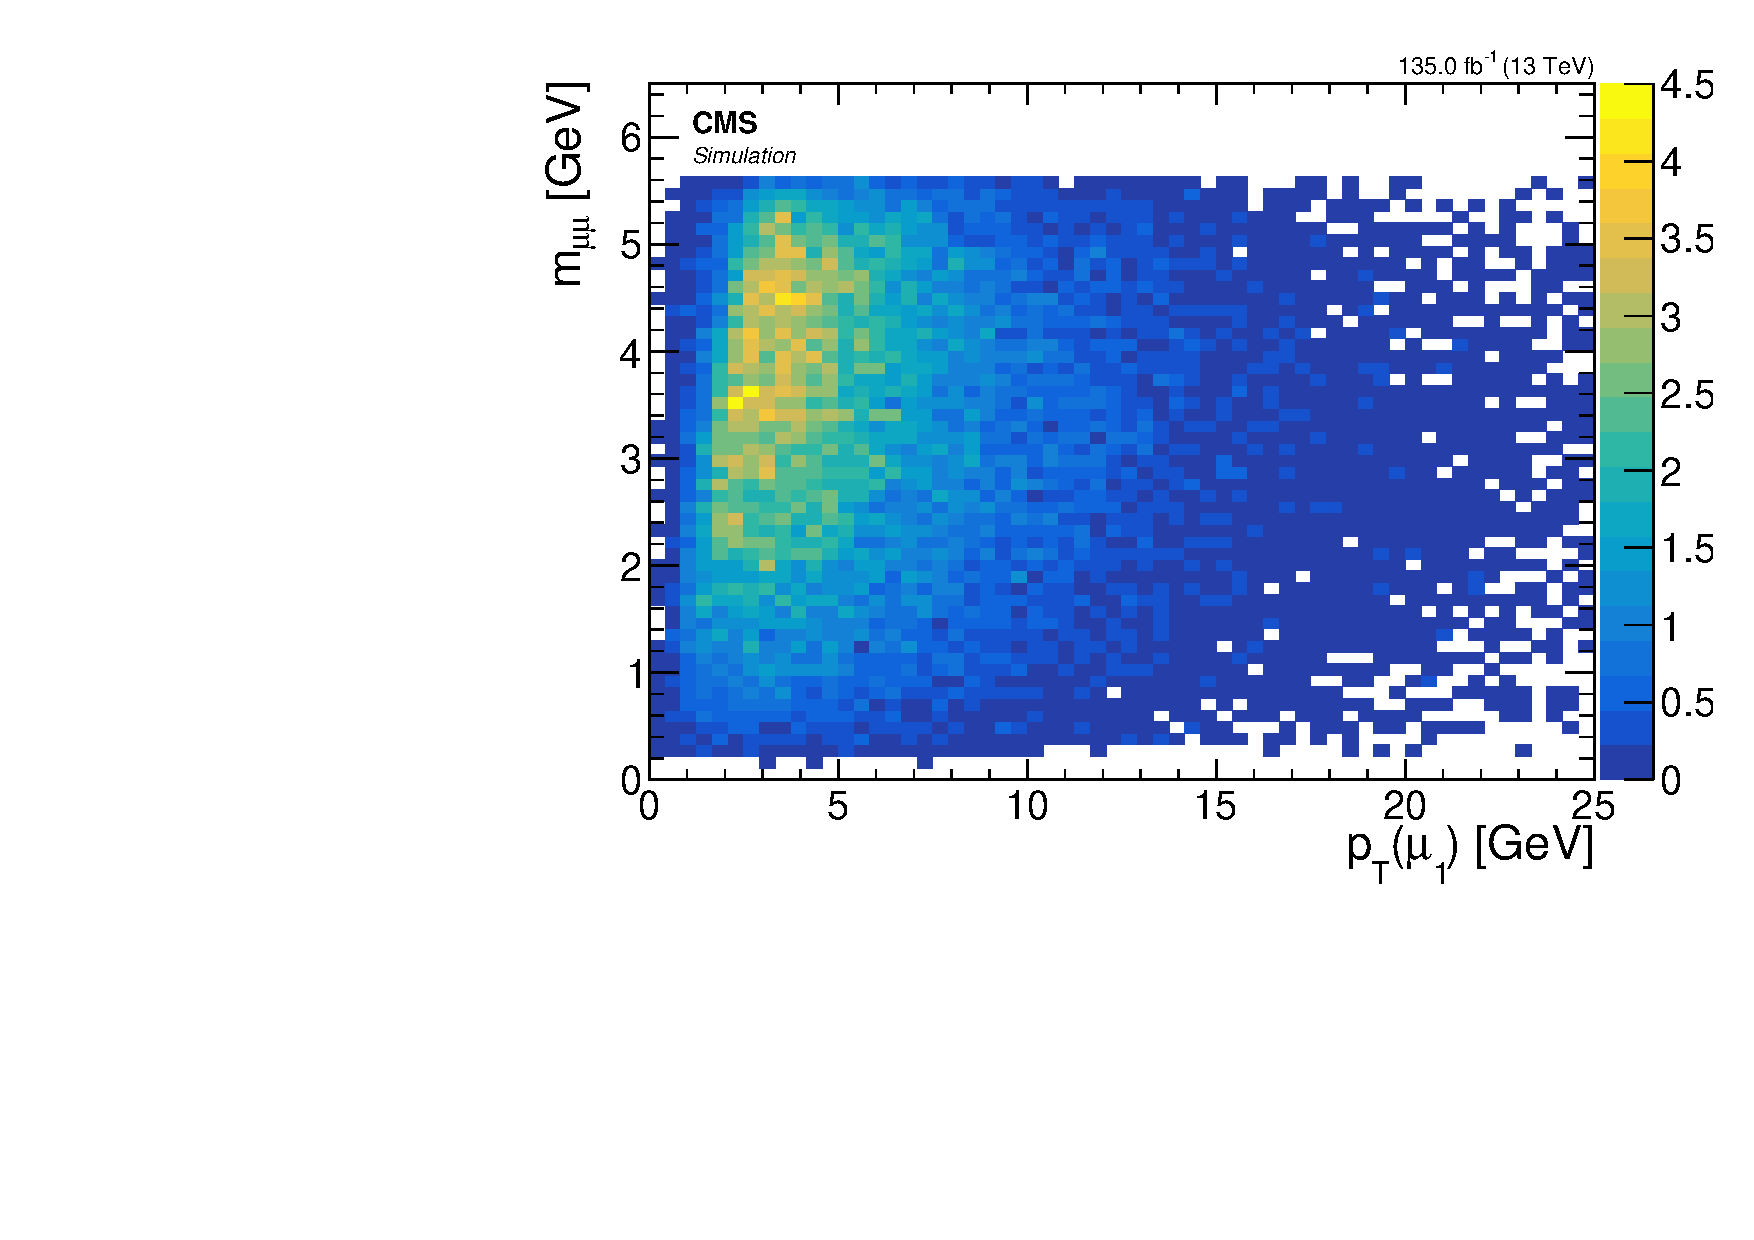
\includegraphics[width=0.48\linewidth]{plots/signal_muons_gen_delta_r_vs_pt_dm5/none_gen_invmass_vs_pt_1.pdf} \,
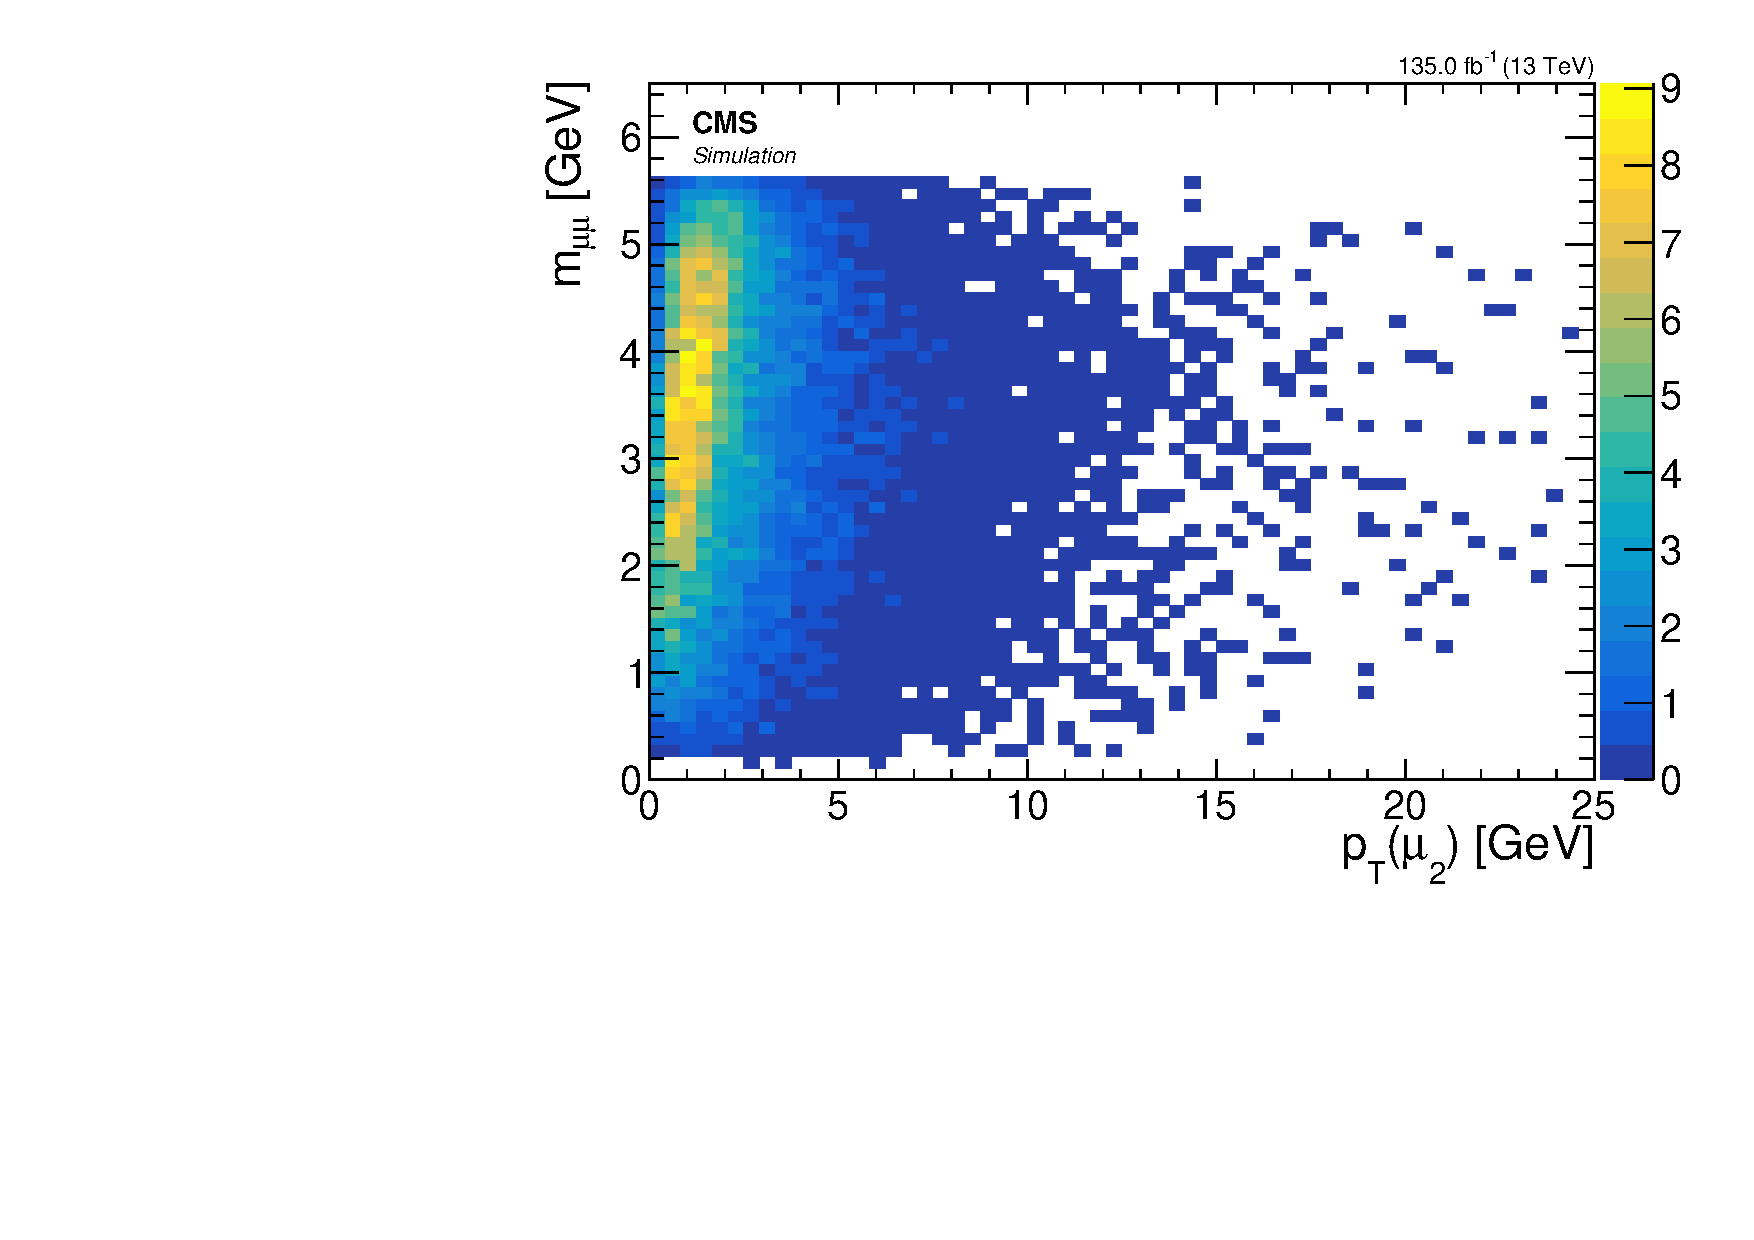
\includegraphics[width=0.48\linewidth]{plots/signal_muons_gen_delta_r_vs_pt_dm5/none_gen_invmass_vs_pt_2.pdf}  \\
\caption[Signal \mmumu \vs \pt]{ Signal \mmumu \vs \pt for leading lepton $\mu_1$ (left) and subleading lepton $\mu_2$ (right) for $\dm=1.13\GeV$ (top) and $\dm=5.63\GeV$ (bottom).}
\label{fig:signal-gen-invamass-pt}
\end{figure}

Earlier, it was established that the invariant mass distribution has an edge at \dm, and the value of \dm can be read from these plots. Another interesting feature to notice in these plots is that there is also a lower edge in the \dm distribution at around $\sim 0.2\GeV$, which is due to each muon having a mass of around $\sim 0.1\GeV$. It is now clear that by cutting on both muons at $\pt\geq 2\GeV$, a significant portion of the signal is lost. This effect becomes particularly substantial for the low $\dm=1.13\GeV$ (top row). The magnitude of this effect is quantified by a cutflow table, where each row represents a cut, and its efficiency is calculated by dividing the number of events passing the cut by the number of events in the previous line. The first line is the baseline of all dimuon events with at least one jet with $\pt \geq 30\GeV$ and $\abs{\eta}<2.4$, and it has an efficiency of 1 by definition. The event number is weighted to Run II luminosity of $\lumi = 135 \fbinv$. The table is shown in~\ref{tab:gen-muon-pt-dr-efficiency}.

\begin{table}[!htb]
	\centering
	\label{tab:gen-muon-pt-dr-efficiency}
		\caption{Generator level efficiency on muons selections}
		%\vspace{1mm}
			\begin{tabular}{l|cc|cc} \hline
			Cut & \multicolumn{2}{c|}{Number of events} & \multicolumn{2}{c}{Efficiency} \\ \hline
			
			 & $\dm=1.13\GeV$ & $\dm=5.63\GeV$ & $\dm=1.13\GeV$ & $\dm=5.63\GeV$ \\
			Baseline & 1710.7 & 1743.9 & 1 & 1\\
			$\pt\geq 2\GeV$ & 24.7 & 724.9 & 0.015 & 0.41\\
			\gls{sos} orthogonality & 24.7 & 490.6 & 1 & 0.68 \\ \hline
			\end{tabular}
\end{table}

It is observed that for the low $\dm$ of $1.13\GeV$, the acceptance of the signal is significantly reduced by the $\pt\geq 2\GeV$ cut, with only $1.5\%$ of the signal remaining. In contrast, the orthogonality condition of requiring $\pt\left(\mu_2\right)\leq~3.5\GeV\text{ or }\drll\leq 0.3$ does not affect it any further. The situation is different for the high \dm of $5.63\GeV$, where the \pt cut is cutting away more than half of the signal and the \gls{sos} orthogonality is cutting an additional two thirds.

It has been established that the \pt distribution directly affects the \mll distribution due to the relationship between the two variables. Thus, it is necessary to investigate how the reconstruction discussed in Section~\ref{sec:muon-eta-pt} might impact the \mmumu distribution. The distributions of the reconstructed \mmumu can be seen in Figure~\ref{fig:reco-signal-invamass}.

\begin{figure}[!htb]
\centering
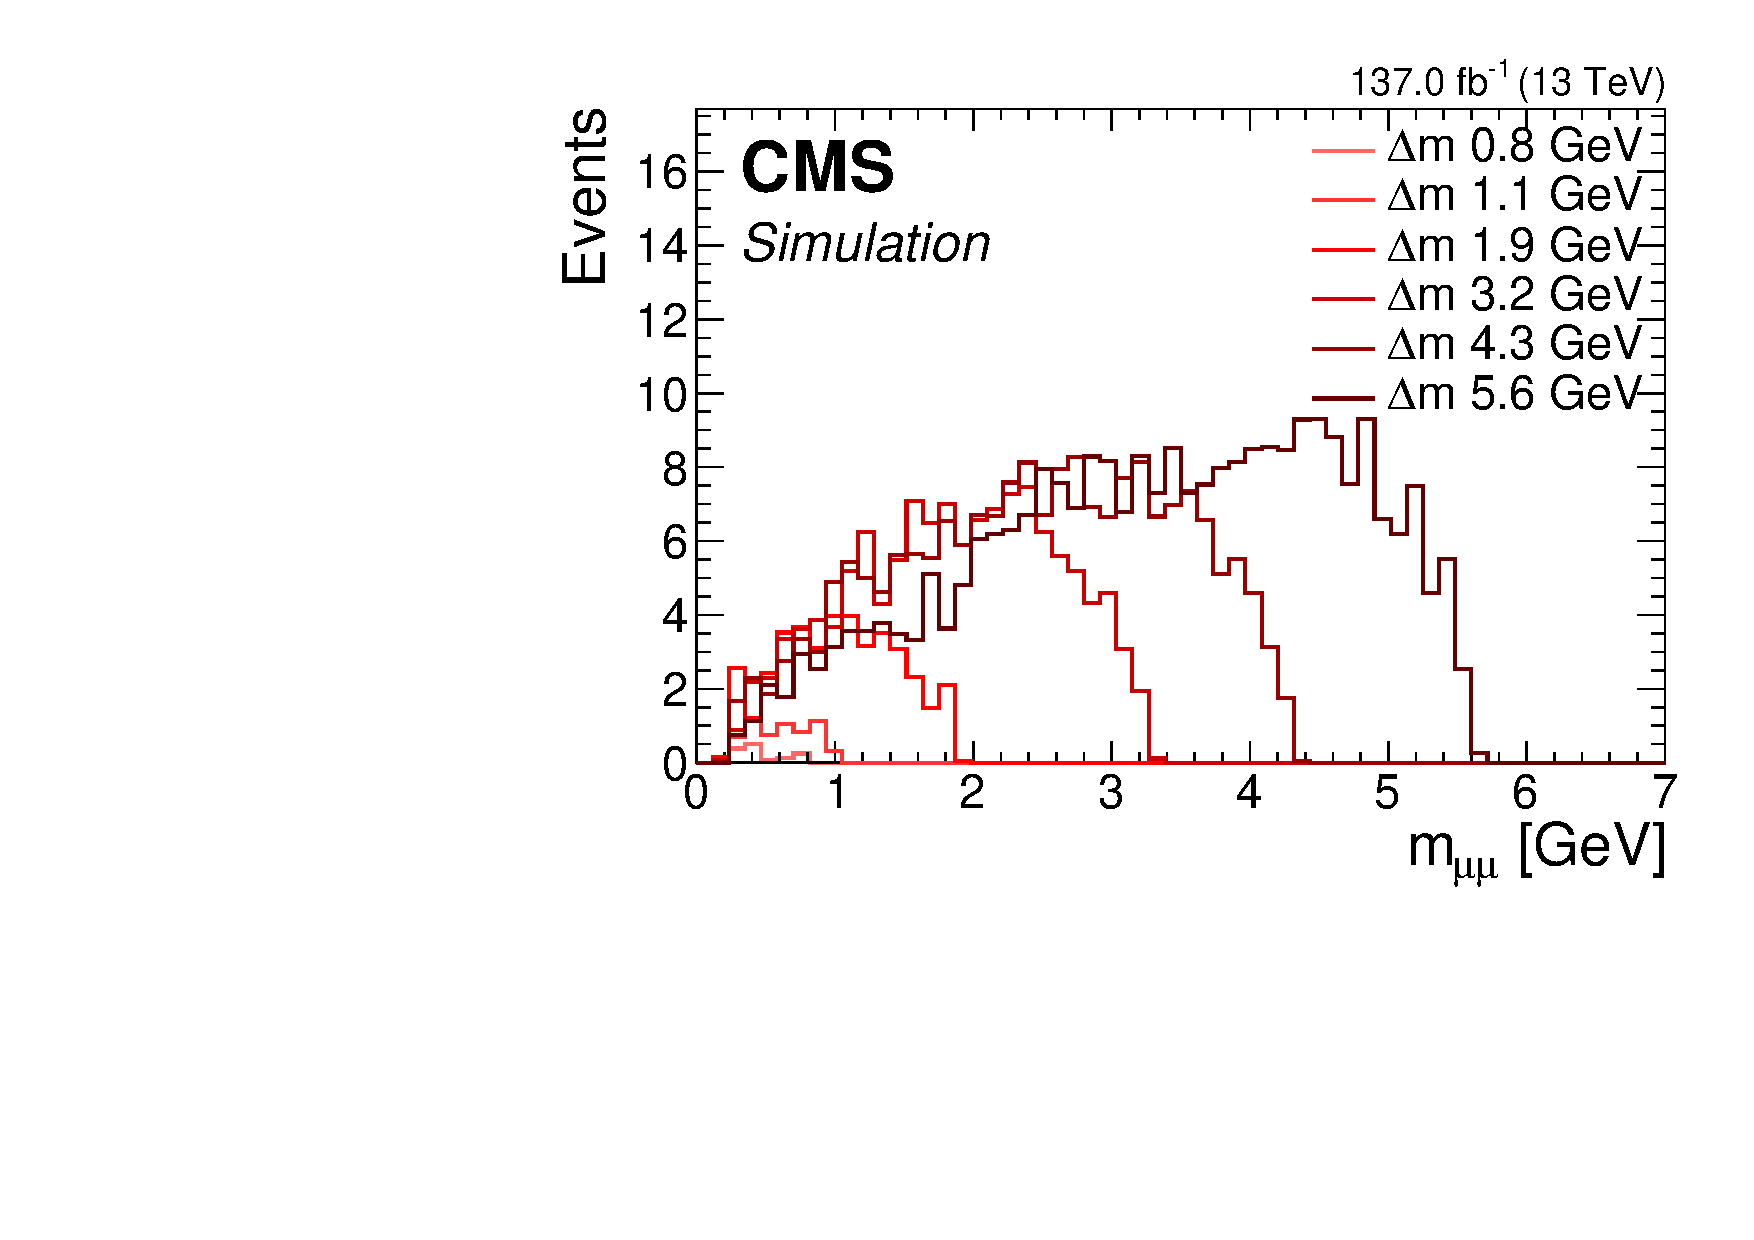
\includegraphics[width=0.48\linewidth]{plots/signal_muons/none_invMassCorrJetNoMultIso10Dr0.6.pdf} \,
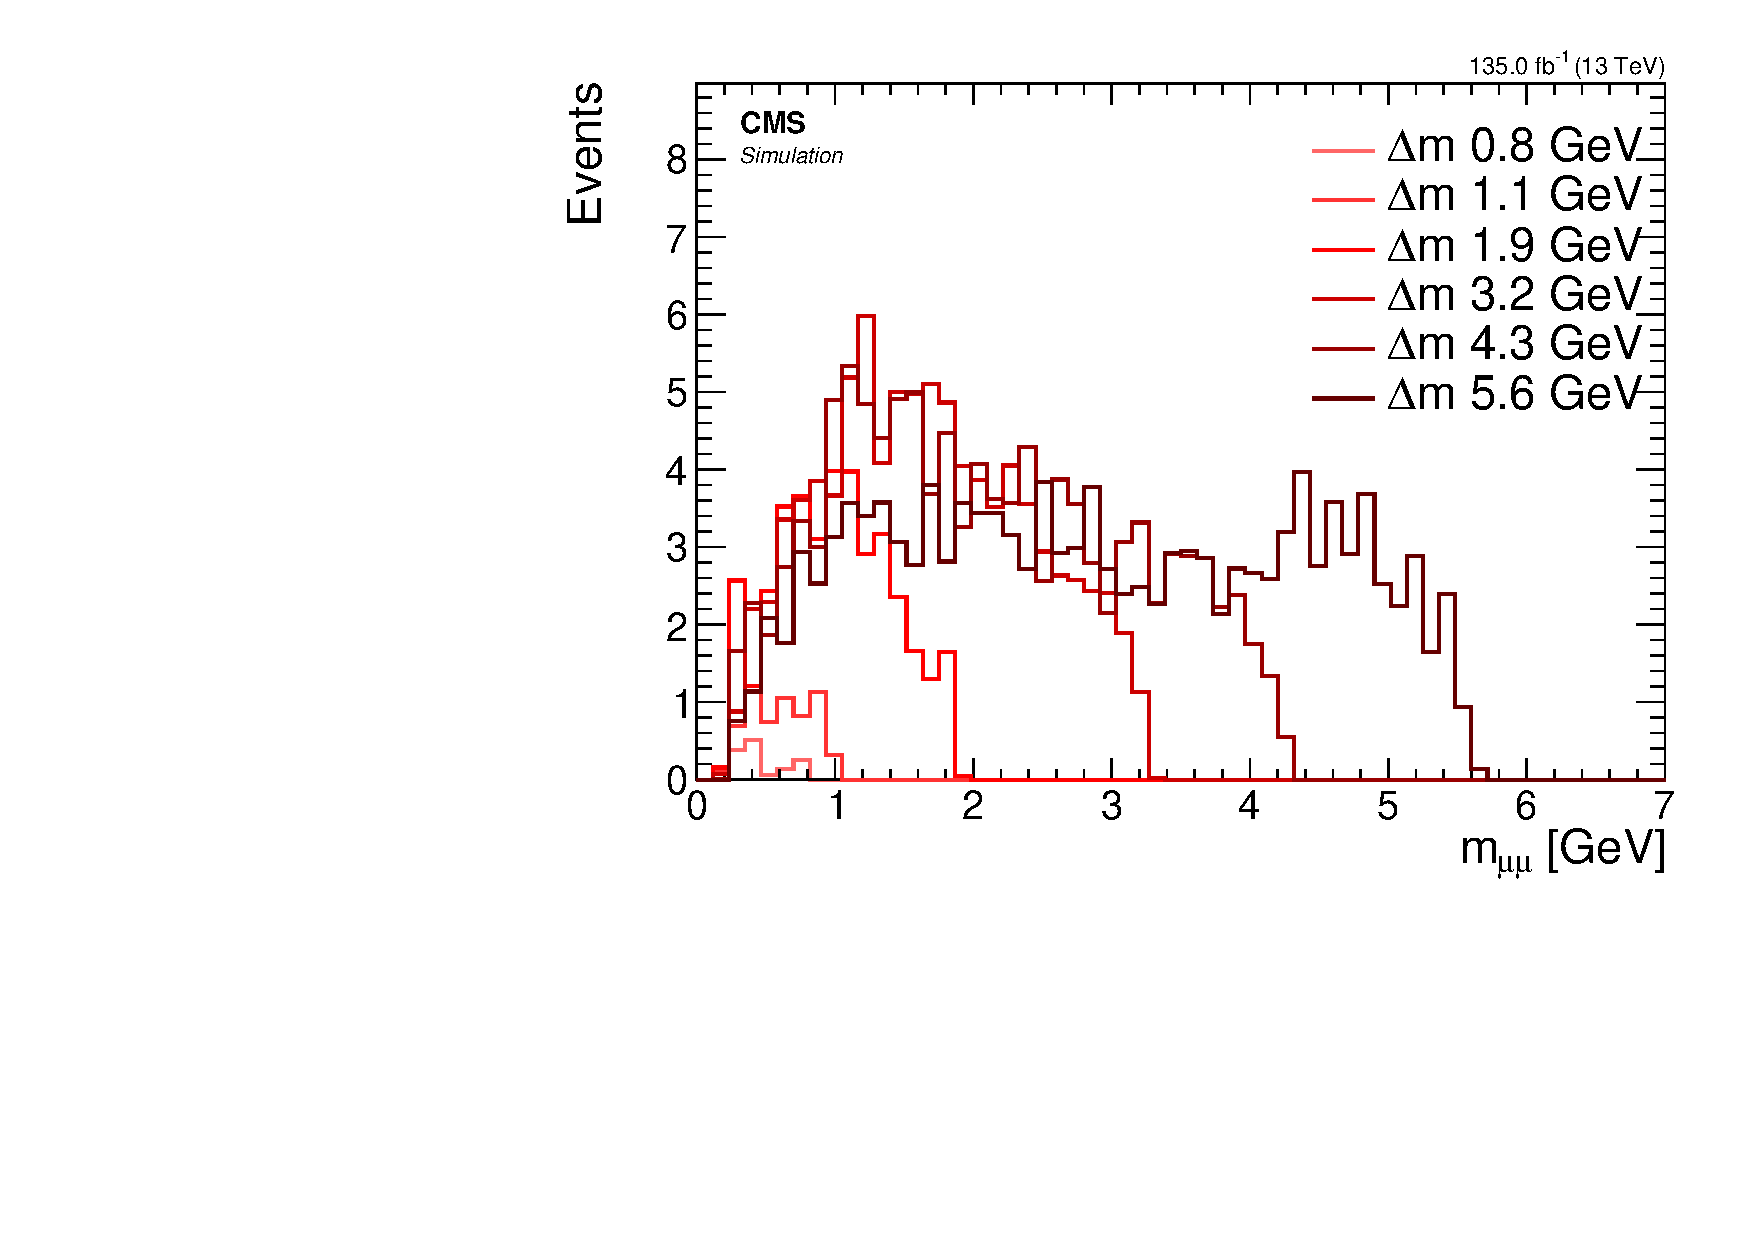
\includegraphics[width=0.48\linewidth]{plots/signal_muons/none_invMassCorrJetNoMultIso10Dr0.6_orth.pdf}  \\
\caption[Signal reconstructed \mmumu]{ Signal reconstructed \mmumu with basic analysis selection (left) and additional \gls{sos} orthogonality condition (right).}
\label{fig:reco-signal-invamass}
\end{figure}

It is interesting to compare these distributions to the two right ones in the generator level version at Figure~\ref{fig:signal-generator-mll}. It can be seen that not only are fewer events surviving the reconstruction, but also some \dm model points are peaking between $1 \GeV$ to $2 \GeV$ with the \gls{sos} orthogonality condition applied.

\subsubsection{Lepton separation \gls{dr}}
\label{sec:lepton-dr}

The lepton separation is defined by the equation $\DR=\sqrt{\left(\deta\right)^2+\left(\dphi\right)^2}$, where \gls{eta} represents the pseudorapidity and \gls{phi} is the azimuthal angle measured in radians. The value of \gls{dr} is significant in this analysis because the produced leptons tend to be located in proximity to each other and therefore are not easily isolated according to standard definitions. Special attention is given to ensuring that the collimated nature of the leptons can be used to differentiate the isolated leptons in the signal from the non-isolated leptons in the \gls{sm} background. It is worth noting that, for the purposes of orthogonality, we attempt to revert the requirement of $\drll > 0.3$ utilized in previous \gls{sos} analyses~\citep{sos}.

Similar to the invariant mass discussed in Section~\ref{sec:gen-invariant-mass}, we examine the distributions of \gls{dr} for various \dm options with different cuts applied to observe their effect.

\begin{figure}[!htb]
\centering
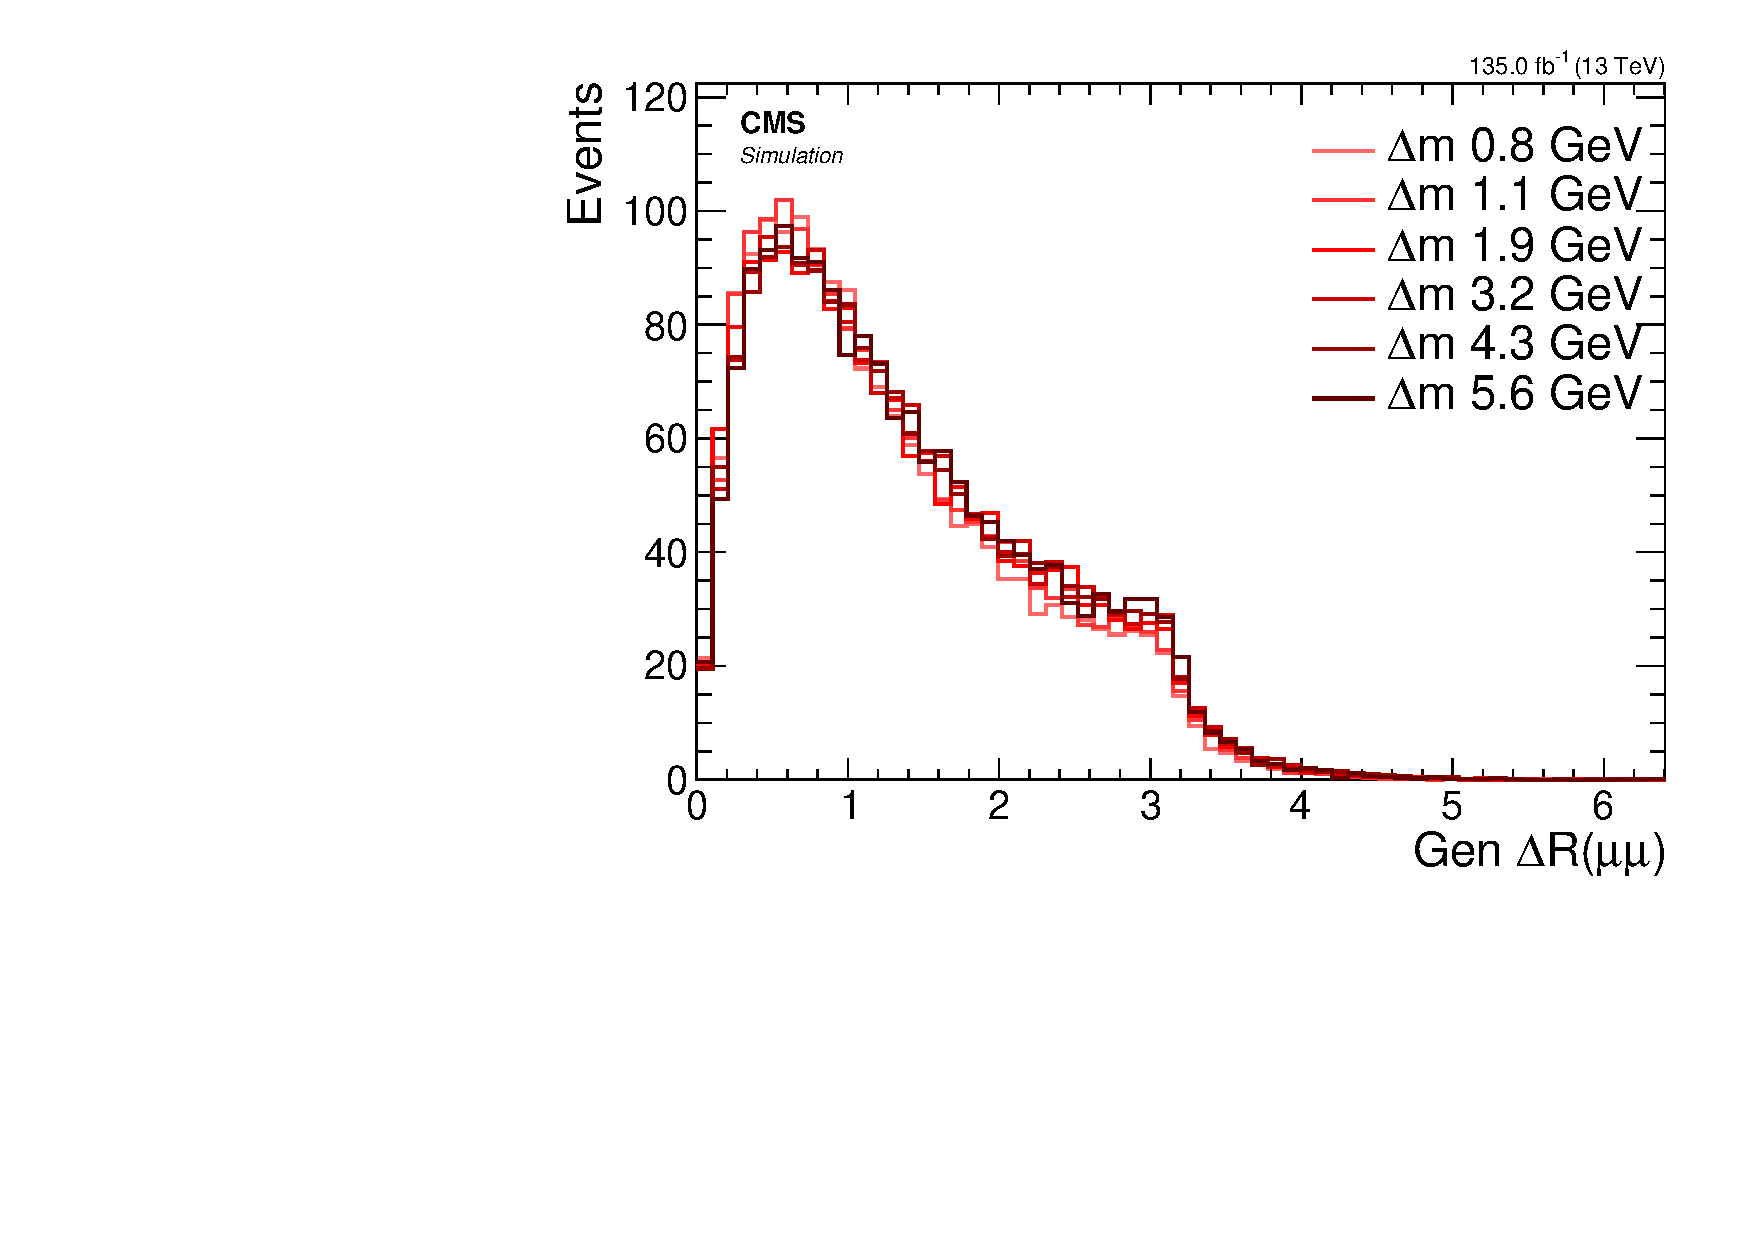
\includegraphics[width=0.32\linewidth]{plots/signal_muons_gen/none_gen_deltaR.pdf} \,
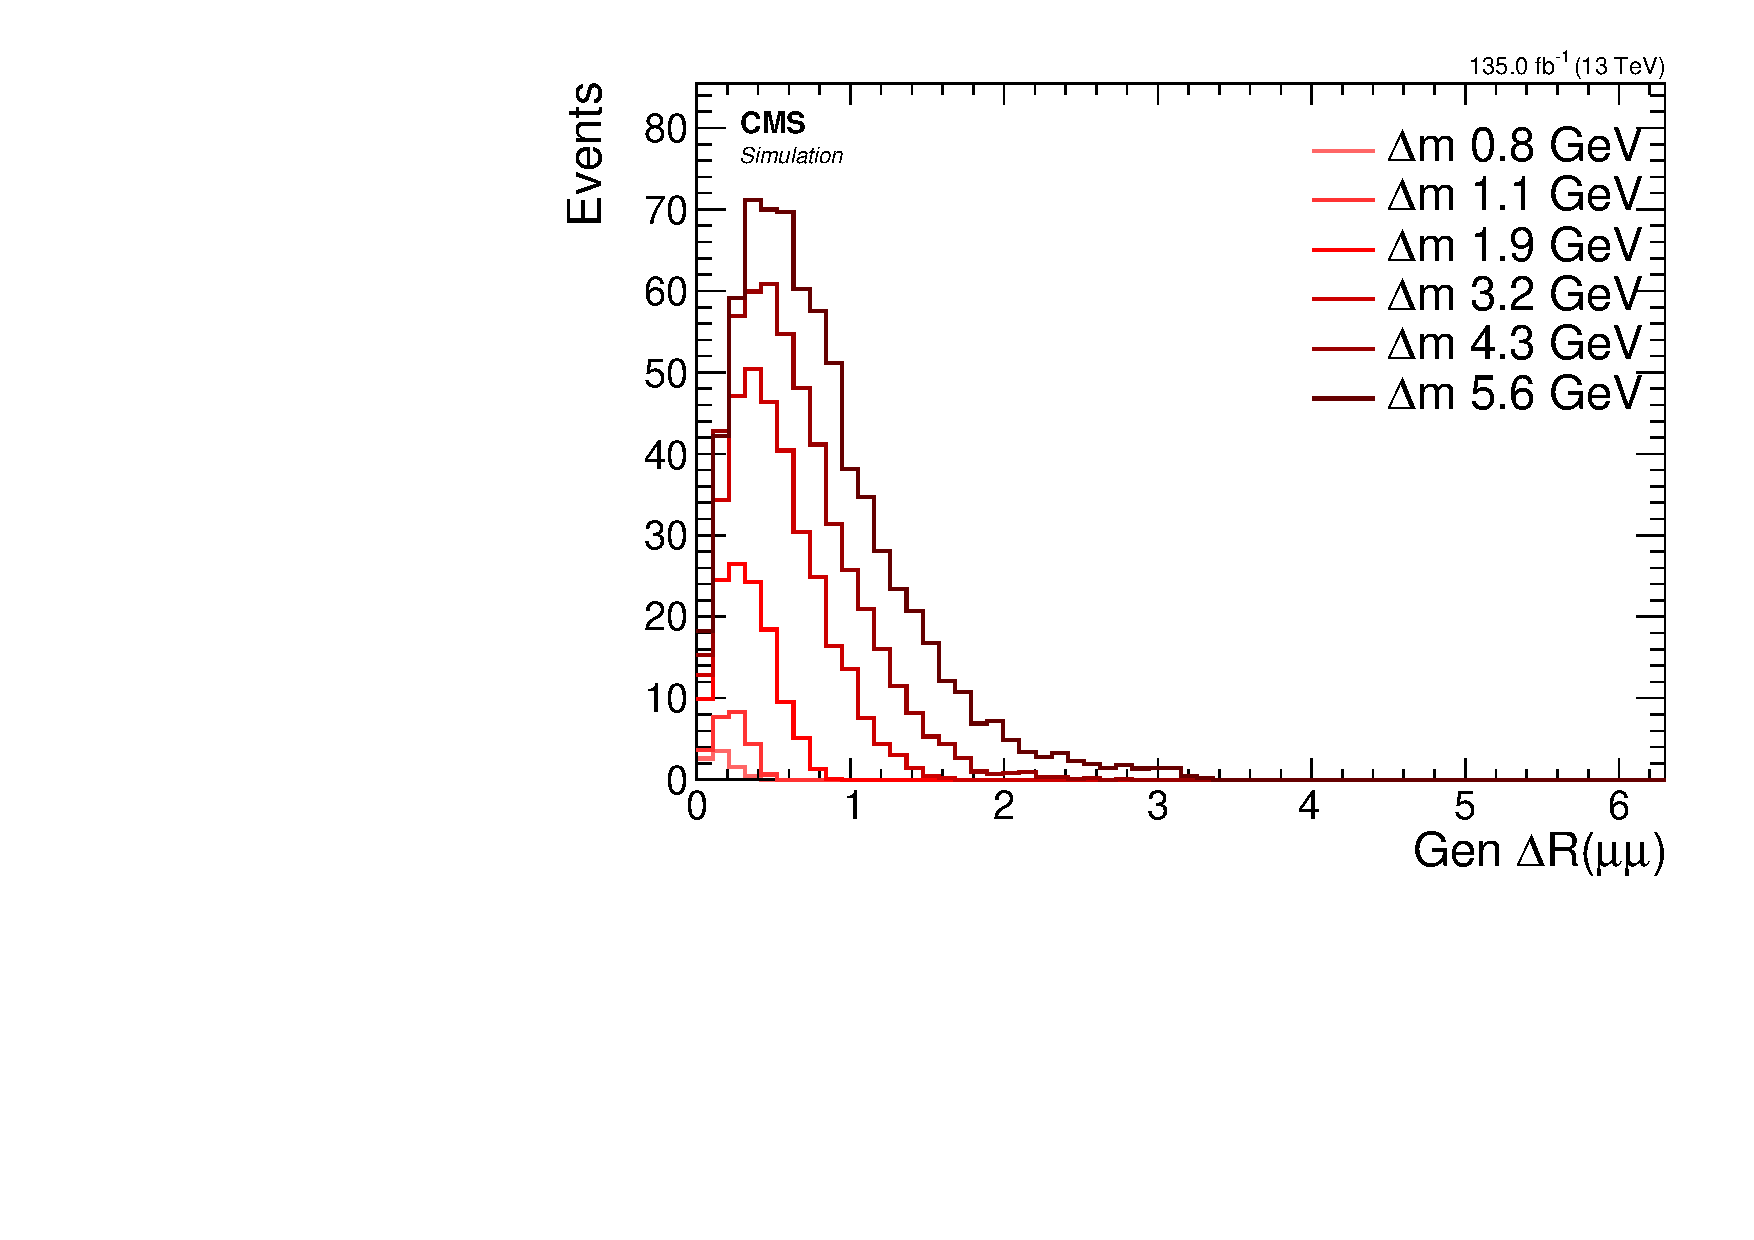
\includegraphics[width=0.32\linewidth]{plots/signal_muons_gen/none_gen_deltaR_cut.pdf}  \,
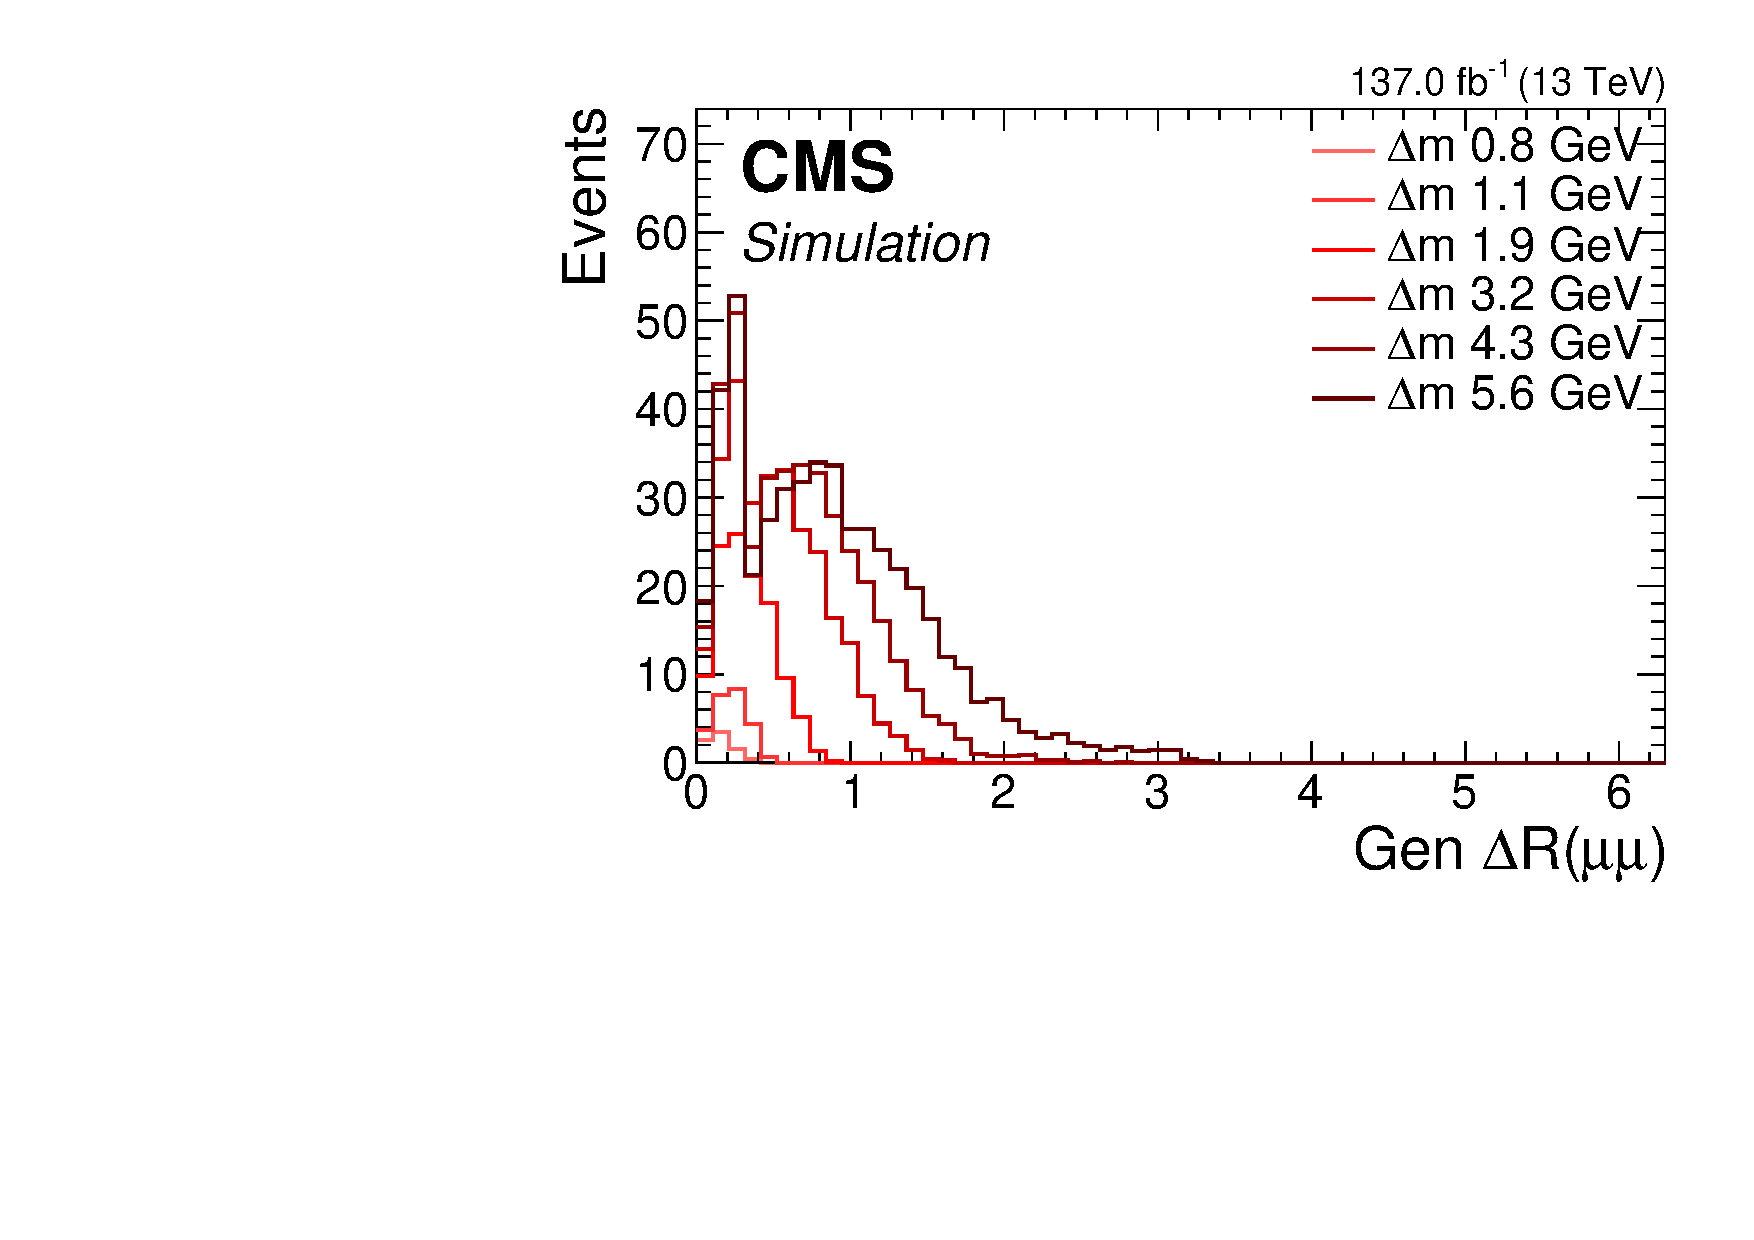
\includegraphics[width=0.32\linewidth]{plots/signal_muons_gen/none_gen_deltaR_orth.pdf} \\
\caption[Signal generator level \DR distributions]{ Signal generator level \gls{dr} distributions with no cuts (left), with $\pt\left(\mu_i\right)>2\GeV,\,i=1,2$ (middle) and with \gls{sos} orthogonality condition $\pt\left(\mu_i\right)>2\GeV$, $\pt\left(\mu_2\right)\leq~3.5\GeV\text{ or }\DR\leq 0.3$ (right).}
\label{fig:signal-generator-dr}
\end{figure}

The left plot of Figure~\ref{fig:signal-generator-dr} shows that roughly the same number of events are produced for all \dm model points. However, when applying a cut of $\pt\left(\mu\right)>2\GeV$, a hierarchy of \dm points emerges, with fewer events as \dm becomes smaller (middle plot). The spike on the right plot is due to the \gls{sos} orthogonality condition, which requires $\drll\leq 0.3$ as one of two conditions in an or statement.

To understand the shaping and hierarchy formation due to the \gls{pt} cut, the \pt of the muons is plotted \vs \drll, as shown in Figure~\ref{fig:signal-gen-dr-pt}.

\begin{figure}[!htb]
\centering
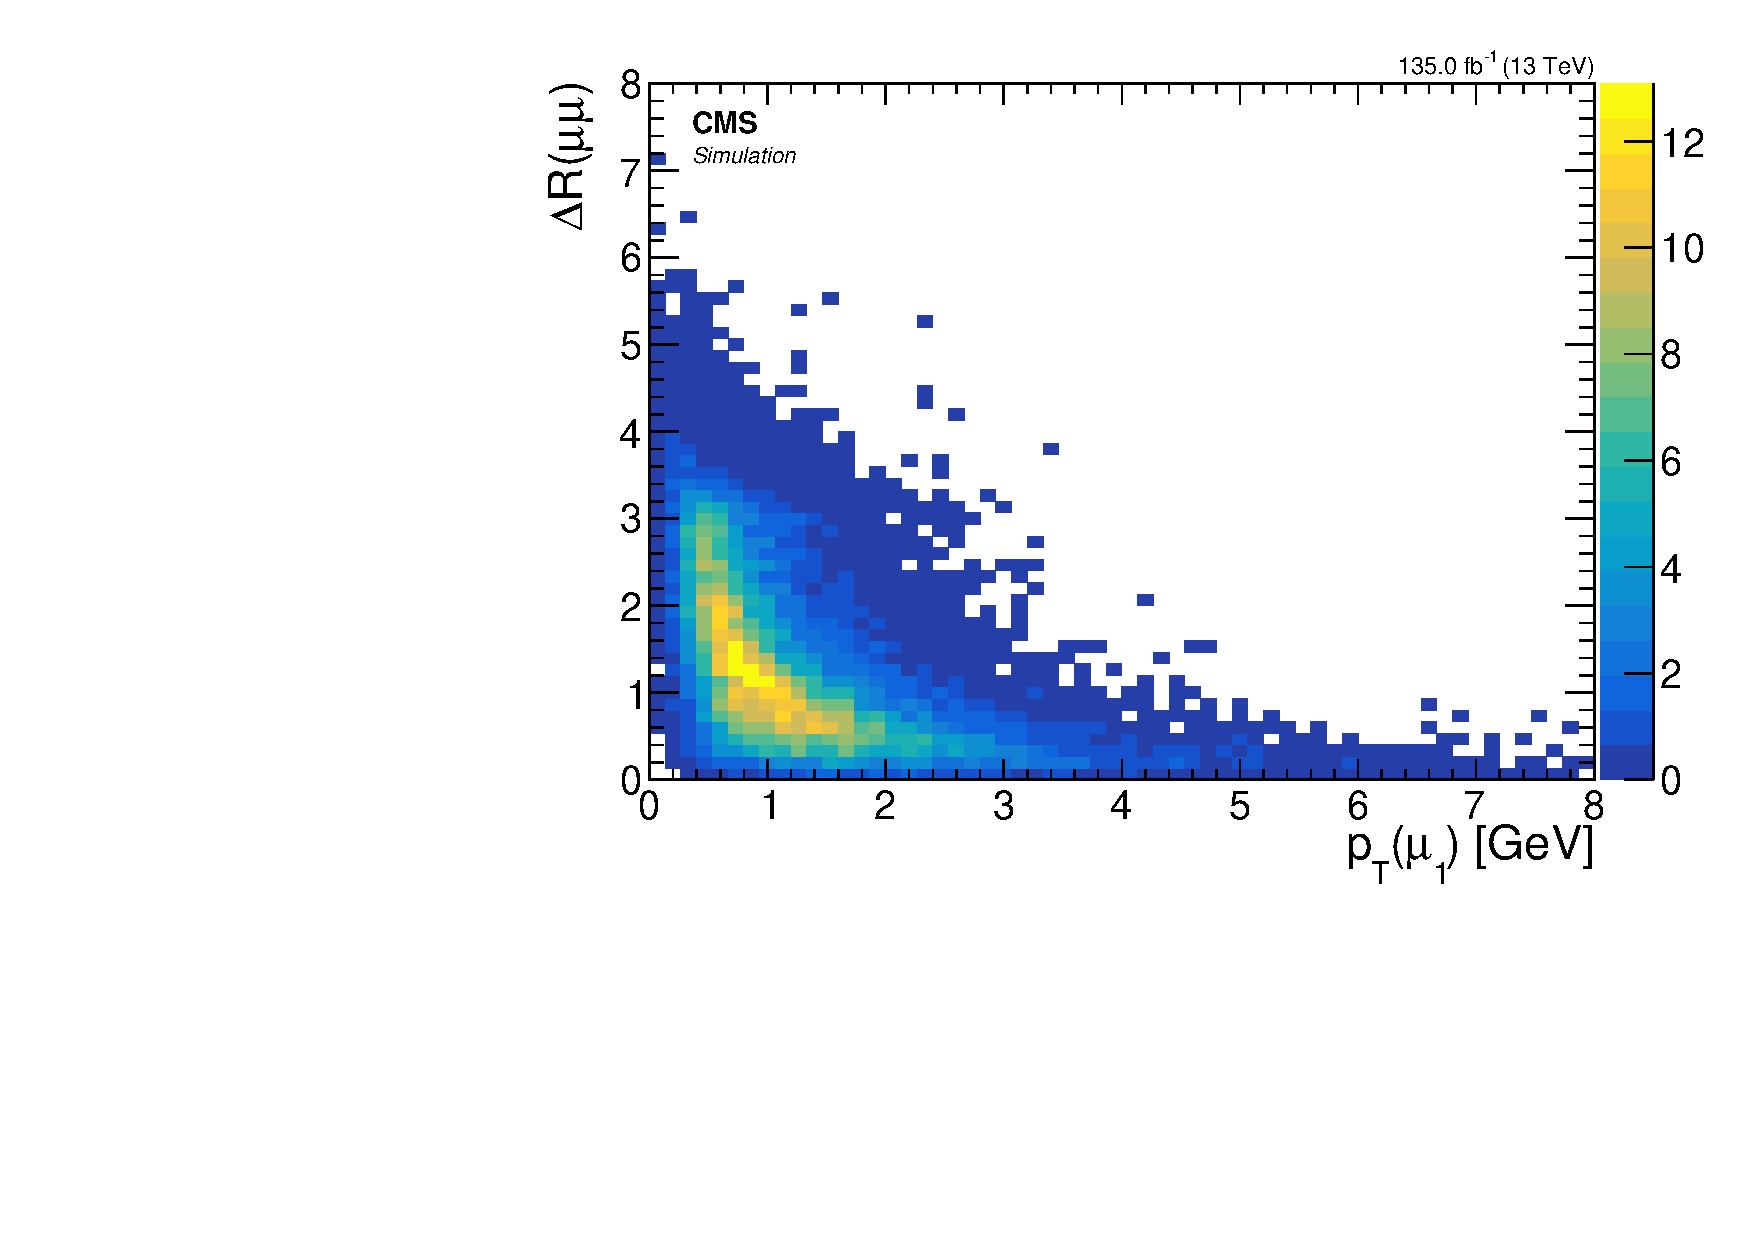
\includegraphics[width=0.48\linewidth]{plots/signal_muons_gen_delta_r_vs_pt/none_gen_delta_r_vs_pt_1.pdf} \,
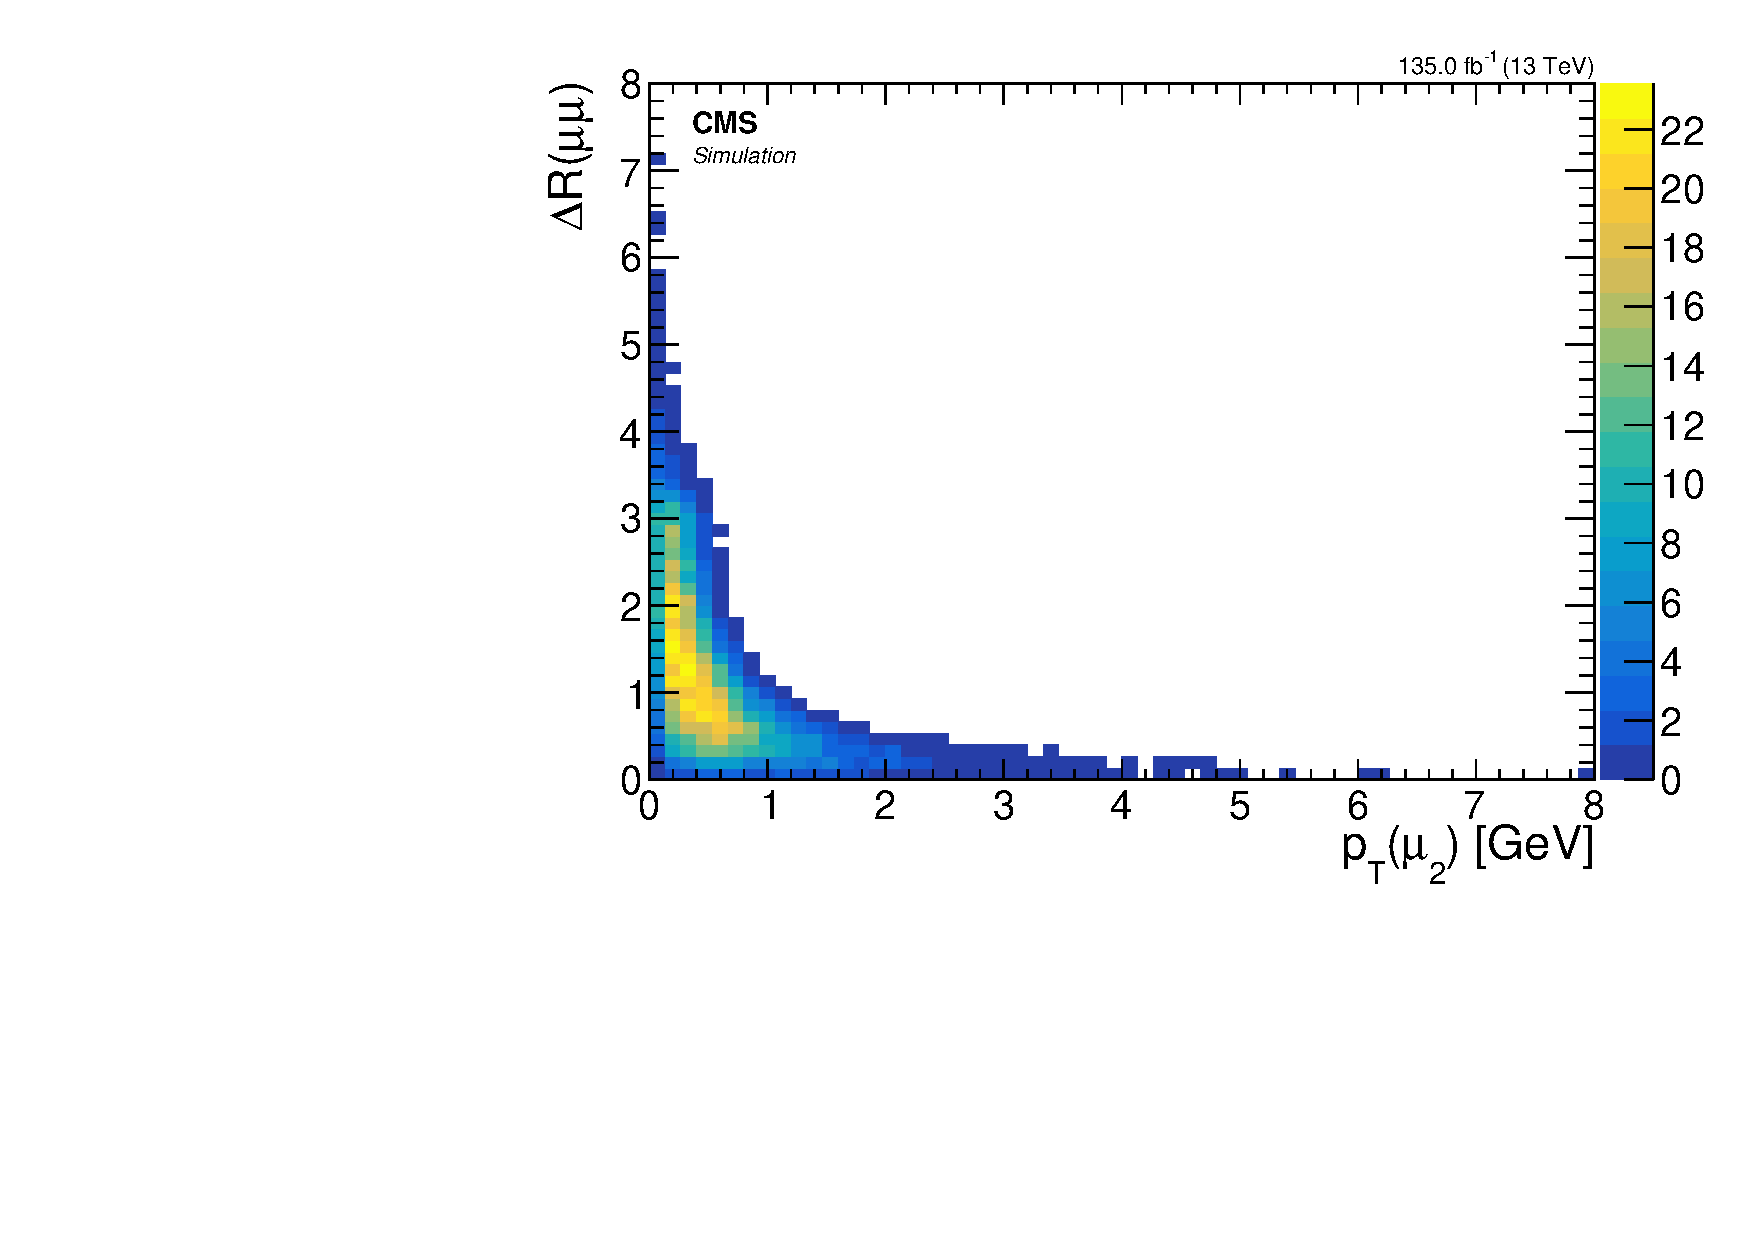
\includegraphics[width=0.48\linewidth]{plots/signal_muons_gen_delta_r_vs_pt/none_gen_delta_r_vs_pt_2.pdf}  \\
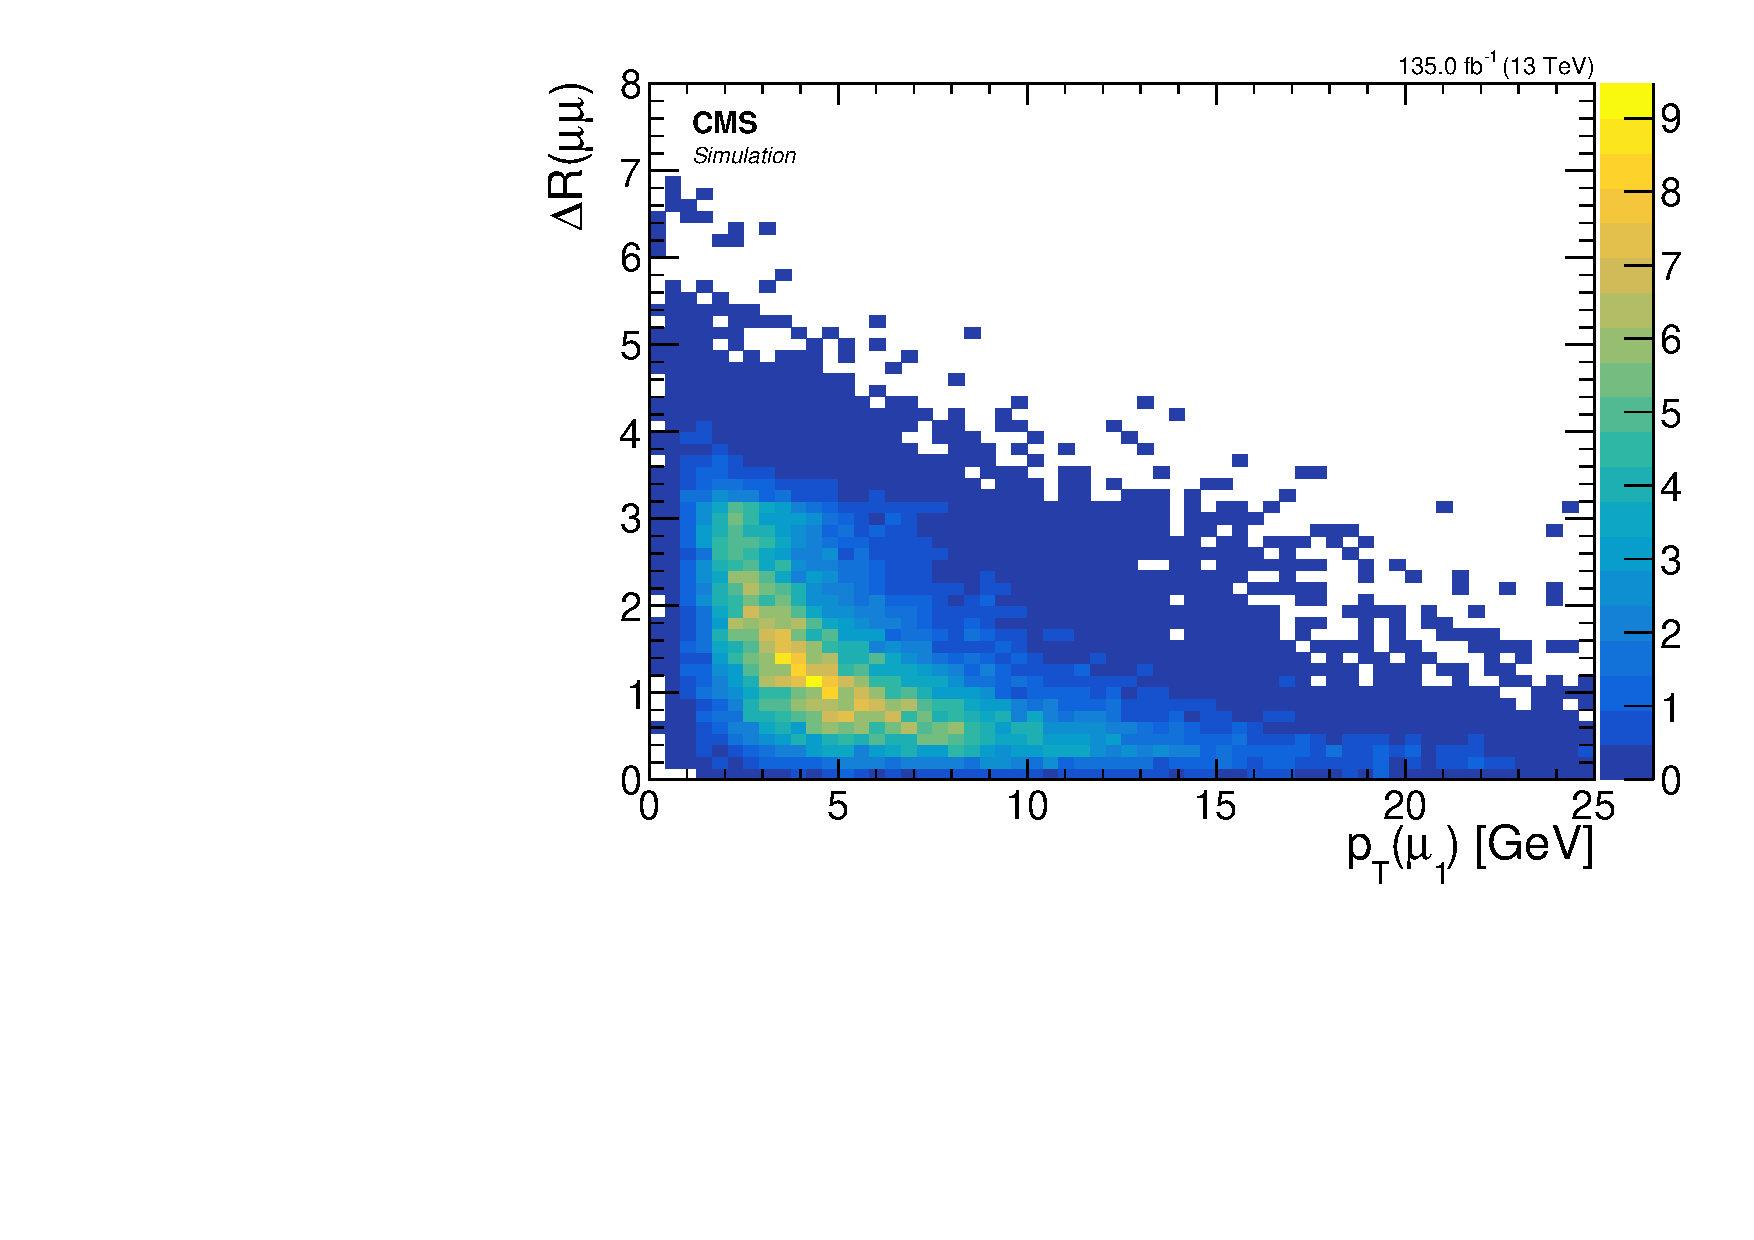
\includegraphics[width=0.48\linewidth]{plots/signal_muons_gen_delta_r_vs_pt_dm5/none_gen_delta_r_vs_pt_1.pdf} \,
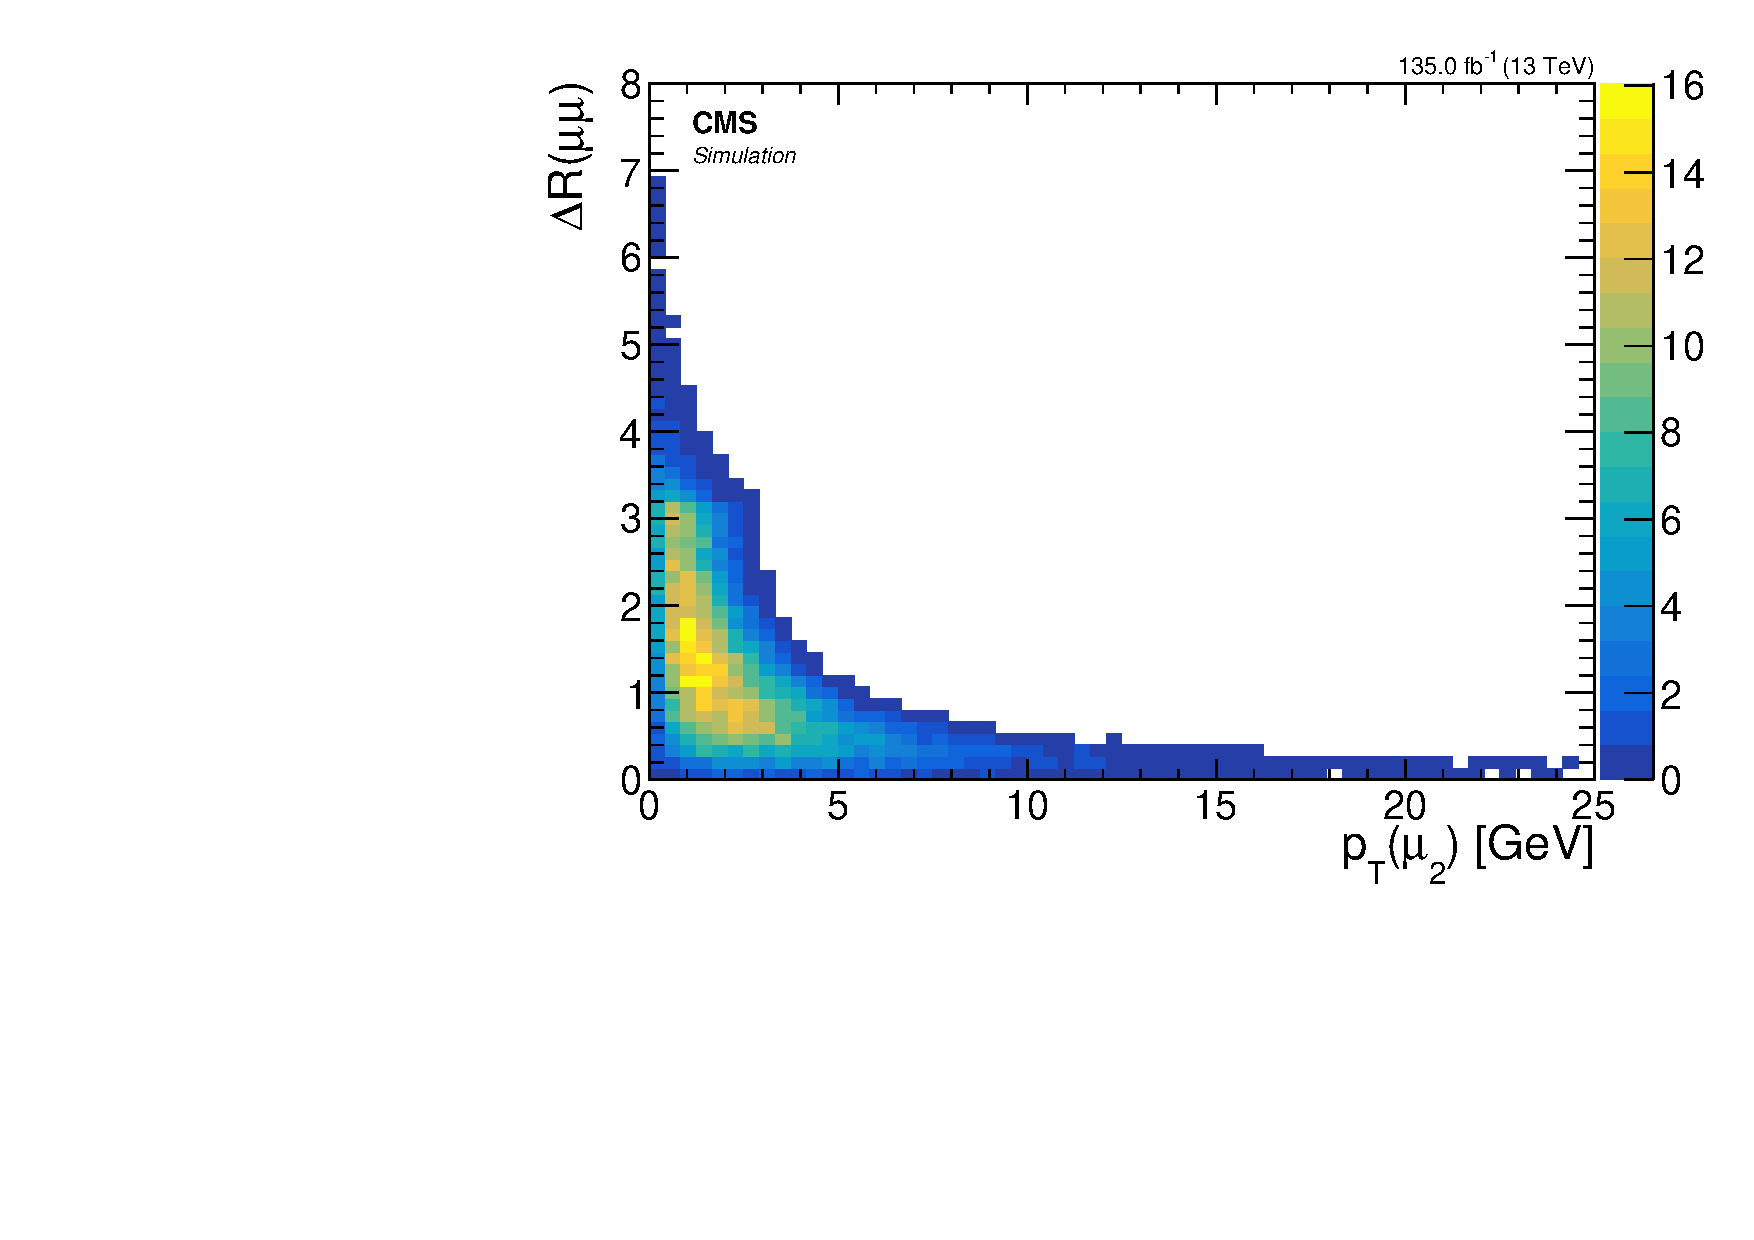
\includegraphics[width=0.48\linewidth]{plots/signal_muons_gen_delta_r_vs_pt_dm5/none_gen_delta_r_vs_pt_2.pdf}  \\
\caption[Signal \drmm \vs \pt]{ Signal \drmm \vs \pt for leading lepton $\mu_1$ (left) and subleading lepton $\mu_2$ (right) for $\dm=1.13\GeV$ (top) and $\dm=5.63\GeV$ (bottom).}
\label{fig:signal-gen-dr-pt}
\end{figure}

The hierarchy can be understood by observing that cutting on $\pt\left(\mu_2\right)\geq 2\GeV$ for $\dm=1.13\GeV$ will limit the range of \drmm to less than $0.4$, while leaving a large range exceeding 3 for the $\dm=5.63\GeV$ model point. It can be concluded that in order to gain access and sensitivity to the low \dm model points, probing low \drll values, potentially with values less than 0.3, is necessary, even before considering the reconstruction efficiency of the leptons. In the next sections, the study of reconstructed leptons and the definition of isolation criteria will enable the retention of signal points with close lepton pairs, as further explored in Section~\ref{sec:isolation}.

As seen in Section~\ref{sec:gen-invariant-mass} for \mmumu, reconstruction has an effect on both the shape and overall count of events. The effects on the \drmm distributions are investigated in Figure~\ref{fig:reco-signal-dr}.

\begin{figure}[!htb]
\centering
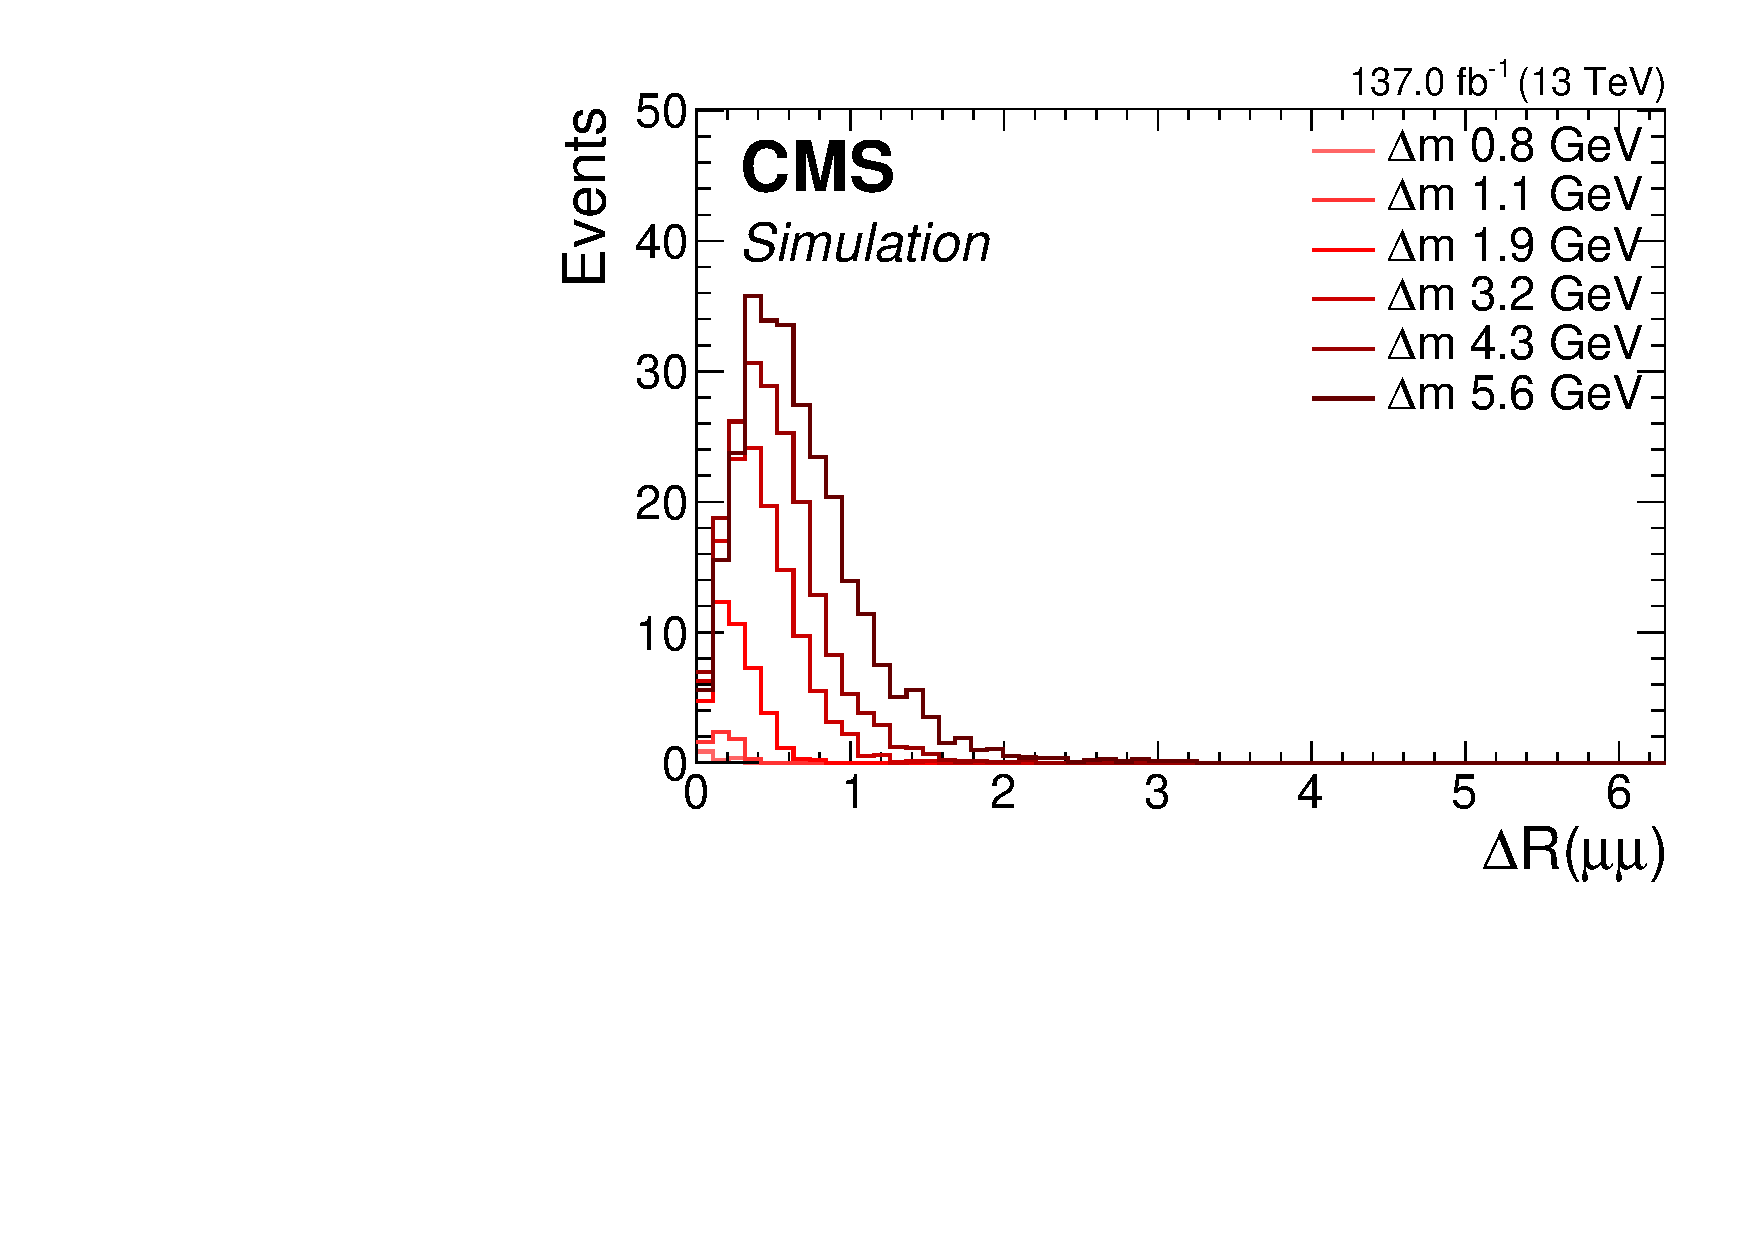
\includegraphics[width=0.48\linewidth]{plots/signal_muons/none_deltaRCorrJetNoMultIso10Dr0.6.pdf} \,
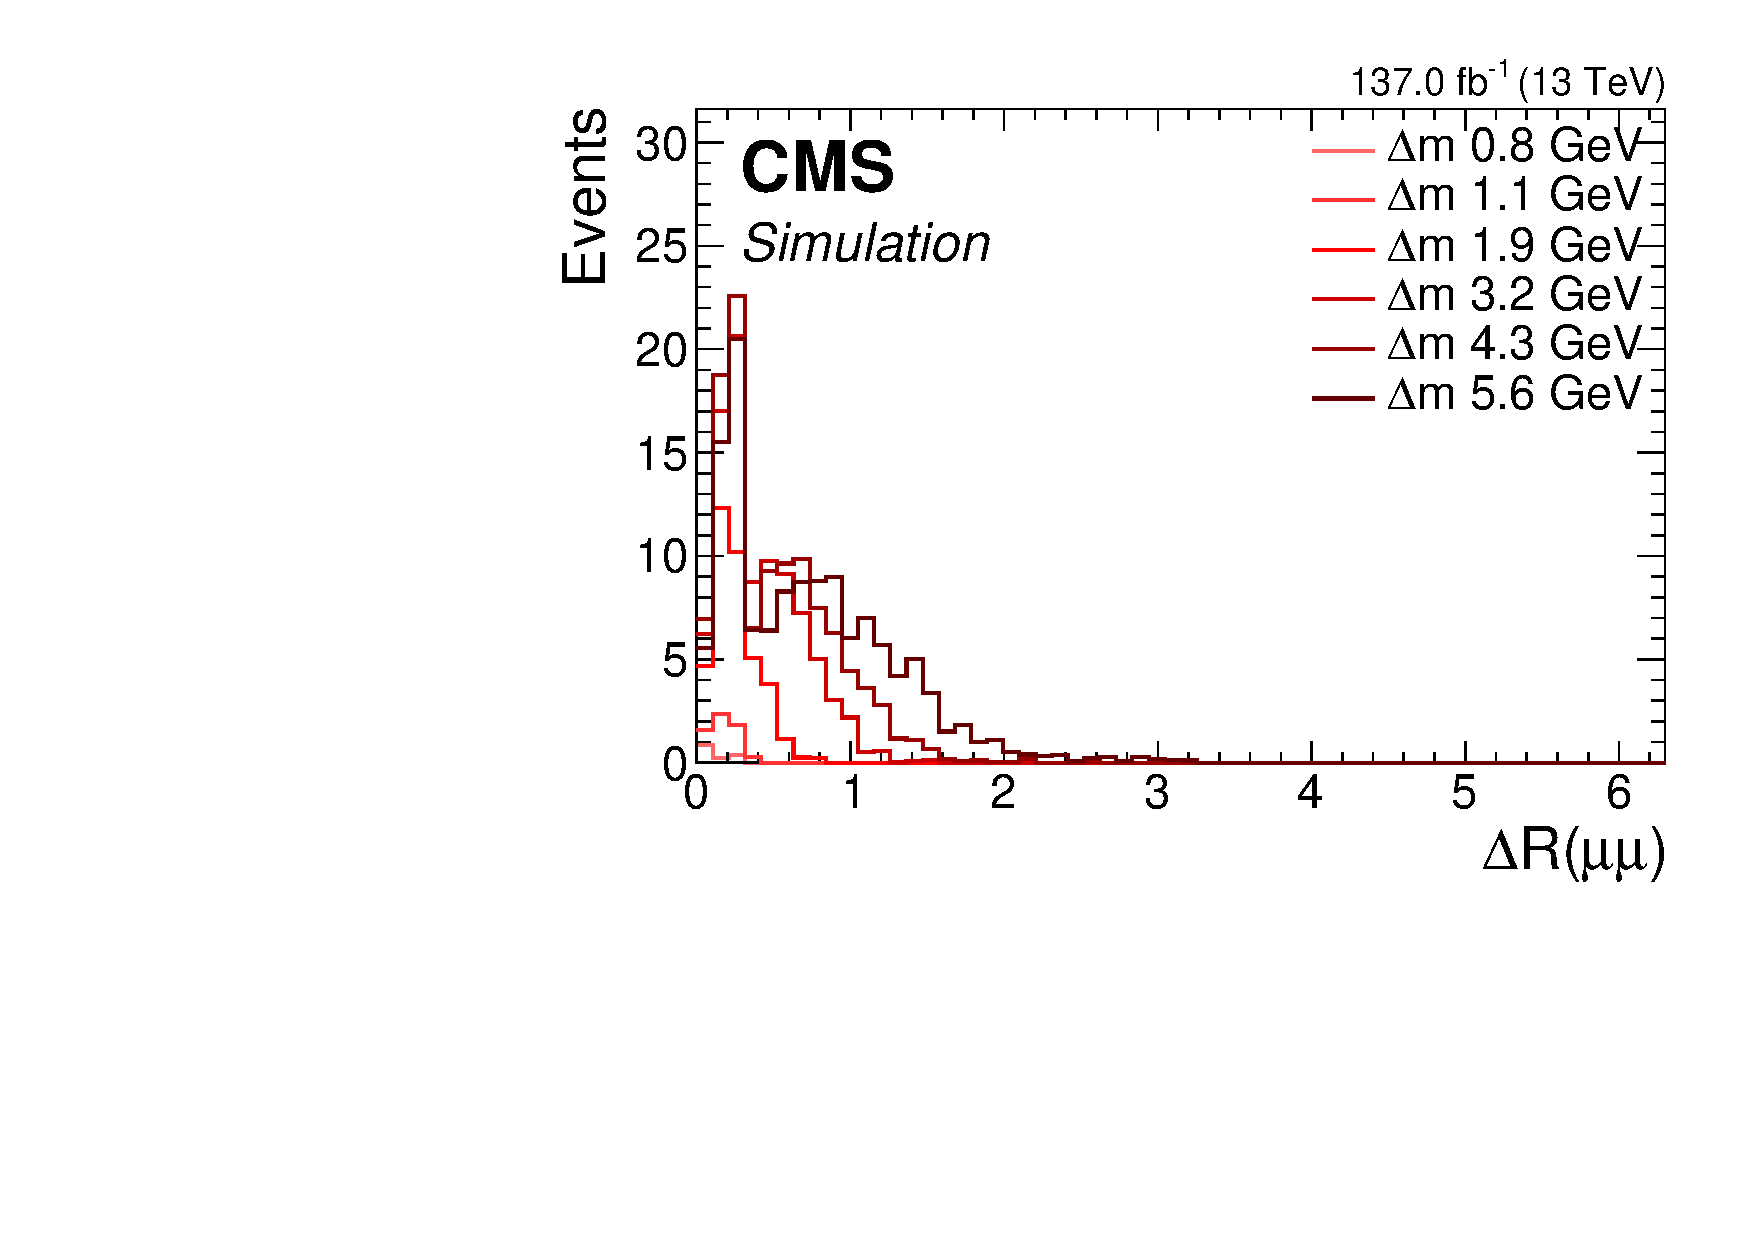
\includegraphics[width=0.48\linewidth]{plots/signal_muons/none_deltaRCorrJetNoMultIso10Dr0.6_orth.pdf}  \\
\caption[Signal reconstructed \drmm]{ Signal reconstructed \drmm with basic analysis selection (left) and additional \gls{sos} orthogonality condition (right).}
\label{fig:reco-signal-dr}
\end{figure}

When the reconstructed \drmm distributions in Figure~\ref{fig:reco-signal-dr} are compared to the generator level ones in Figure~\ref{fig:signal-generator-dr}, it can be observed that the main effect of the reconstruction on the \drmm is the overall normalization, which is due to reconstruction efficiency.

\clearpage 
\subsection{Main drivers of sensitivity}

Conclusions can be drawn from this signal distribution studies in regards to the main drivers to the sensitivity of different model points of this analysis, as well as of future analysis that might try to expend on this one. This section does not consider \gls{sm} background at all, making it hard to conclude what effects changing the cuts to \MET or other event level observables might have. However, one thing is very clear from examining the dilepton kinematics, and that is to gain access to low \dm model points, the threshold on the \pt of the decay leptons must be lowered and low \gls{dr} must be probed. Another driver of the sensitivity at all \dm model points is the luminosity, since the production cross section drops as a function of the higgsino mass parameter $\mu$.

The next sections will explore how to lower the threshold on the muons transverse momentum and deal with collimated leptons that might pose a challenge in regards to the isolation criterion.
